% /////////////////////////////////////////////////////////////////////////////
%
%   Ph.D. Thesis Manuscript -- Pruthvi Mehta
%
% /////////////////////////////////////////////////////////////////////////////


% /////////////////////////////////////////////////////////////////////////////
% PREAMBLE
  %\documentclass
\documentclass[11pt,twoside]{report}
\renewcommand{\appendixname}{}%
  % for title page
  %\title{Neutral-Current Quasi-Elastic events with neutron tagging at Super-Kamiokande}
  \author{Pruthvi Mehta}
  \date{2022}




  %%%%%%%%%%%%%%%%%%%%%%%%%
  %       PACKAGES        %
  %%%%%%%%%%%%%%%%%%%%%%%%%
  % Graphics and Figures
  \usepackage{graphicx}                % Graphics importing library
  \usepackage{float}                   % Placement of floats
  \usepackage[font=small]{caption}     % Set formatting options for captions
  \usepackage{subcaption}              % Like captions, but for sub-figures
  \usepackage{wrapfig}                 % Wrap text around figures
  \usepackage[headheight=14pt,inner=4cm,outer=2.5cm]{geometry} % The minimal margins as specified by Code of Practice.
  \usepackage{setspace}
  \usepackage{datetime}
  %\usepackage{fancyhdr}
  \usepackage{tikz}
  \usepackage{floatpag}
  \usepackage{lscape}
  \usepackage[compact]{titlesec}
  \raggedbottom
  \usepackage[titletoc]{appendix}
  \usepackage{placeins}
  \usepackage{epigraph}
  
  


  % Tables
  %\usepackage{arydshln}                % dashed version of cline
  \usepackage{array}                   % Do more fancy things with tables
  \newcolumntype{L}{>{$}l<{$}} % math-mode version of "l" column type
  
  \usepackage{multirow}                % Let cells span multiple rows
  %\usepackage{longtable}               % For tables that span multiple pages (remove if not needed)
  \usepackage{booktabs}                % Make tables look better
  \usepackage{makecell}
  \newcommand{\mc}{\multicolumn{1}{c}}
  \usepackage{hhline}

  % Maths
  \usepackage{amsmath}                 % Makes maths look pretty
  \usepackage{amssymb}                 % Something to do with symbols...
  \usepackage{xfrac}                   % Pretty inline fractions
  \usepackage{bbold}
  \usepackage{chemformula}
  \usepackage{gensymb}

  \usepackage{setspace}                % Double spacing for easy reading 
  %\doublespacing{}
  \onehalfspacing

  % Hyperlinks & Colors
  %\usepackage[usenames, dvipsnames, table]{xcolor}

  % Fonts
  \usepackage{anyfontsize}             % Setting of font size by point
  \usepackage{cite}                    % Make citations looks pretty

  % Misc
  \usepackage{lipsum}                  % Lorem ipsum generator, good for imagining writing
  \usepackage[nohyperlinks]{acronym}   % Acronym support
  \usepackage[displaymath, mathlines]{lineno}
  %\usepackage[backend=biber,
  %            style=numeric,
  %            backref=true,
  %            bibencoding=utf8,
  %            url=false,
  %            doi=true,
  %            isbn=false
  
  


  
  
  
  %\AtEveryBibitem{\clearfield{note}\clearfield{addendum}\clearfield{annotation}} 
  %\AtEveryCitekey{\clearfield{note}\clearfield{addendum}\clearfield{annotation}}


  %%%%%%%%%%%%%%%%%%%%%%
  %       FONTS        %
  %%%%%%%%%%%%%%%%%%%%%%
 % \usepackage{fontspec}                       % Use of system fonts
 % \setmainfont{Crimson Text}[
 %   Ligatures=TeX,
 %   SmallCapsFont=Crimson,
 %   SmallCapsFeatures={Letters=SmallCaps}
  %]
  %\setsansfont[Ligatures=TeX]{Helvetica}      % Set sans-serif font

  % Change to 2 to comply with UGS requirements
  %\renewcommand{\baselinestretch}{1.15}

  %\usepackage[hidelinks=true]{hyperref}

  \usepackage{hyperref}
  \hypersetup{colorlinks,
              citecolor=blue,
              filecolor=blue,
              linkcolor=blue,
              urlcolor=blue
  }

  \makeatletter
  %% Insert your title and name.
  \Huge
  \title{\textbf{NCQE Interactions as a background to DSNB events with neutron tagging at SK-Gd}} \let\Title\@title
  \author{Pruthvi Hiren Mehta} \let\Author\@author
  \makeatother


  %/////////////////////////////////////////////////////////////////////////////
  % DOCUMENT

\begin{document}
%\pagestyle{empty}

\begin{titlepage}
	\centering
	\vspace*{1cm}
	
\includegraphics[width=65mm]{Figures/UoL_Logo.jpg}\par\vspace{1cm}
		\vspace{2cm}
	{\huge \Title\par}
	\vspace{2cm}
	{Department of Physics \par}
	{University of Liverpool \par}
	\vspace{2cm}
	{Thesis submitted in accordance with the requirements of the University of Liverpool for the degree of Doctor in Philosophy by  \par}
	\vspace{1cm}
	{\textbf{\Author}\par}
	\vfill

% Bottom of the page
	{\large \monthname\, \the\year\par}
\end{titlepage}
%\cleardoublepage



%% In the preface, pages are numbered by roman numerals (i,ii,...) and in the header Author and Title.
\pagenumbering{roman}
%\pagestyle{fancy}

%\cleardoublepage
%\thispagestyle{empty}

    % Typeset title page.
    %\maketitle


    % Include front matter
\chapter*{Dedication}
\thispagestyle{empty}
\chapter*{In Memoriam}
\thispagestyle{empty}
\begin{center}
    
\includegraphics[width=0.2\textwidth]{Figures/om.png}
\end{center}

\vspace*{\fill}
\noindent
\hspace*{-\oddsidemargin}%
\begin{center}
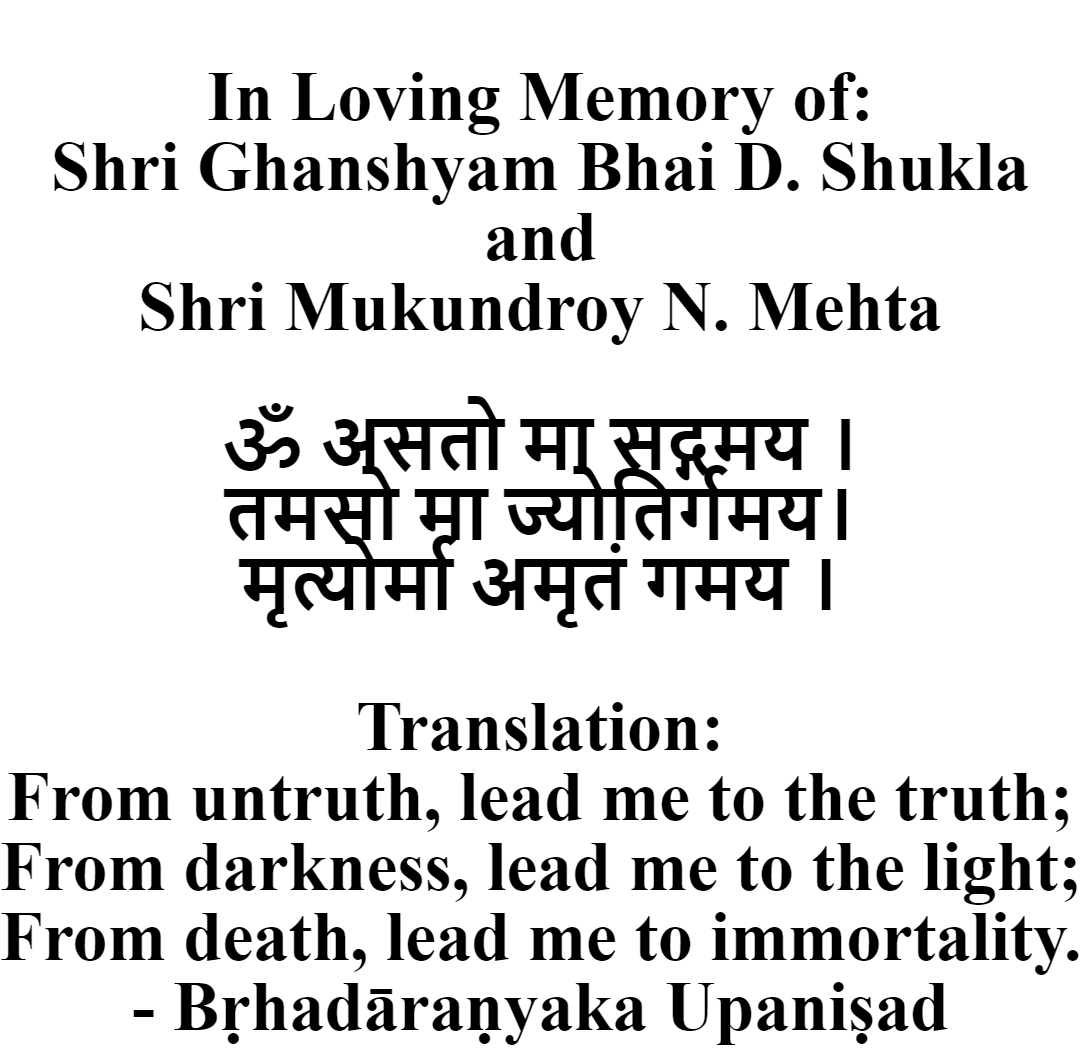
\includegraphics[width=0.6\textwidth]{Figures/memoriam.png}
\end{center}
\vspace*{\fill}
\chapter*{Acknowledgements}
\thispagestyle{empty}
First and foremost thanks must be given to my academic supervisor Professor Neil McCauley, someone whose intelligence, work ethic and kindness have continously been a source of inspiration to me. 

I am also forever indebted to a number of postdoctoral researchers who I was fortunate enough to have aid me with my research; namely Dr Ka Ming Tsui, Dr Pablo Fernandez Menendez, Dr Lauren Anthony, Dr Adrian Pritchard and Dr Samuel Jamuel Jenkins. Thank you all for your continued encouragement and support, and apologies for emailing all of you for help so much (but in my defence ROOT is the worst).

I am also incredibly grateful to members of the neutron tagging working group, in particular Dr Fabio Iacob whose weekly meetings about my analysis were crucial to my work and who is one of the most patient and kind individuals I have ever met (and I wouldn't have survived calculating the systematics without him). I am also indebted to Seungho Han for his help with the new neutron tagging software, and also Nakajima-sensei, Koshio-sensei, Akutsu-sensei and Tairafune-san for their input in the neutron tagging meetings. 

I'd also like to thank current and former members of the Super-Kamiokande and Hyper-Kamiokande calibration groups, Dr Jordan McElwee, Dr Matthew Thiesse, Dr Billy Vinning and Yang-san for UKLI MC implementation help. 
 
A huge thank you to Dr Gedminas Elertas, who has been a source of virtue and intellectual inspiration to me and has made me want to keep learning, not just with things relating to physics but outside of it too. The day-to-day of academic research sometimes ground me down a little internally, but you kept the spirit of scientific curiosity alive inside me, and I can't thank you enough for this. 

Many thanks to my wonderful besties from undergrad, Karel Green and Rachel Couchman, I've known both of you for nearly a decade and I treasure your friendship so so much, you've kept me sane and supported throughout this entire journey. Here's to you, babes!
Also to my schoolfriends Catherine Thomas, Amy Rose-Mansbridge and Catriona Bradley, I've known you for over 15 years and it has been incredible to see you all blossom into amazing, capable and talented young women who I'm blessed to know. Also thanks to Patrick Bates for the calmness and profound wisdom that you so often espouse, you wonderful lovely nerd! 

Thank you to Joseph (my \textit{imzadi}) for your gentle and kind heart, you've always been so incredibly supportive and I'm so happy to know you.  

To my parents, ``thank you'' isn't anywhere near a sufficient enough response to how much you've supported me. Mum - your strength and wisdom is unparalled, and dad, well, you're the best physicist I know. Finally to my sister Nidhi, who this thesis is dedicated to, I love you so much and your kindness and intelligence is something I aspire to everyday. You're amazing! 

\chapter*{Abstract}
\thispagestyle{empty}
    % \include{acronyms}

\tableofcontents

\cleardoublepage
\pagenumbering{arabic}
    % Include body text
  \chapter{Introduction}
\label{chp:intro}

\section{Introduction}

\subsection{Neutrino Physics}

There are a plethora of physics phenomenon in which neutrinos are involved, including beta decay, cosmic rays, and supernovae. As part of the Standard Model, they are descibed as being Dirac fermions with no electric charge with three flavours: the electron neutrino, the muon neutrino and the tau neutrino, corresponding with their associated leptons: the electron, muon and tauon. Prior to the discovery of neutrino oscillations, it was believed that neutrinos were massless, but they in fact have small but non zero masses (<1eV). The next subsections of this chapter will discuss a brief history of neutrino physics including the discovery of neutrino oscillations, the manner in which neutrinos interact with nuclei in the Super-Kamiokande detector, and the motivation behind an NCQE neutron tagging analysis.

\subsection{History of Neutrino Physics}

To correct a violation of energy conservation discovered in beta-decay, Wolfgang Pauli put forward the idea of a neutrino (Italian for "little neutral one") as a solution. In 1934, Enrico Fermi's theory of beta decay stated that a neutron could decay to a proton, electron and an antielectron neutrino and in 1956, Clyde Cowan and Frederick Reines directly confirmed the existence of neutrinos, by detetecting the electron antineutrino originating from inverse beta decay produced from a nuclear reactor. In inverse beta decay (shown in Equation \ref{eq:IBD_eq}), an electron antineutrino interacts with a proton to produce a neutron and positrons. These positrons pair-annihilate with electrons and produce two 0.5 MeV gamma rays which go in opposite directions. Scintillator material was placed in a tank of water, which was used to detect the gamma photons, and the scintillator light produced flashes of visible light which were detected by photomultiplier tubes. Cadmium chloride was used to detect the coincident neutron, which after exciting and de-exciting, emits a gamma ray within 5 microseconds after the pair-annihilation gammas are detected. In 1962, Ledermen, Schwartz and Steinberger detecting the muon neutrino, and in 2000 the DONUT collaboration at Fermilab detected the existence of the tau neutrino. 

In the 1960s, the Homestake experiment made the first measurement of solar electron neutrino flux. These are produced by nuclear fusion using the proton-proton chain reaction, where four protons are converted into neutrinos, alpha particles, positrons and energy. The experiment used a perchloroethlene-based detector, placed 1,478 metres underground in the Homestake Gold Mine in South Dakota. When an electron neutrino interacts with 37Cl in the perchloroethlene, the 37Cl becomes a radioactive isotope of 37Ar which are extracted by bubbling helium through the tank, and then counted in order to determine how many neutrinos had been captured. The theoretical solar neutrino flux calculated by John Bachall was about three times as much as Raymond Davis' results from the experiment: with Bachall's calculations predicting a solar neutrino flux of $7.9 \pm 2.6$ SNU, whereas the Homestake experimental results showed a flux of $2.1 \pm 0.3$ SNU. These results were consistent with those from the Kamiokande, SAGE and GALLEX experiments.
\newline
The solution to this problem came from the Super-Kamiokande and Sudbury Neutrino Observatory experiments. In 1998, Super Kamiokande showed evidence of neutrino oscillation: where muon neutrinos produced by cosmic rays in the upper atmosphere changed into tau neutrinos within the Earth, pointing to the fact that the deficit in the solar neutrino flux oberved at Homestake, SAGE and GALLEX had to do with neutrino oscillation. In 2001 SNO observed the flux of electron neutrinos but also the flux of all flavours of neutrinos, and found that the fraction of electron neutrinos was found to be 34\%, perfectly concordant with the prediction.

\subsection{Neutrino Oscillation}
In 1957 Bruno Pontecorvo postulated that neutrinos could transition from neutrinos to antineutrinos and vice versa (similarly to how two kinds of neutral kaons ($\bar{K_{0}}$, and $K_{0}$ were found to oscillate.) Neutrino flavour oscillation theory was then developed by Maki, Nakagawa and Sakata in 1962. The PMNS matrix (Pontecorvo-Maki-Nakagawa-Sakata matrix), the neutrino analogue of the Cabbibo-Kobayashi-Masakawa quark mixing matrix. 
Equation \ref{eq:neutrino_osc} shows the relationship between the mass and flavour eigenstates for a neutrino with a definite flavour of $\alpha$ and a definite mass of $m_{i}$.

$$
\begin{aligned}
&\left|\nu_{\alpha}\right\rangle=\sum_{i} U_{\alpha i}^{*}\left|\nu_{i}\right\rangle \\
&\left|\nu_{i}\right\rangle=\sum_{\alpha} U_{\alpha i}\left|\nu_{\alpha}\right\rangle
\end{aligned}
\label{eq:neutrino_osc}
$$


In Equation \ref{eq:neutrino_osc}, the terms $U_{\alpha i}^{*}$ and $U_{\alpha i}$ are the complex conjugate and normal PMNS matrix. Equation \ref{eq:PMNS_matrix} shows the 3x3 form of the PMNS matrix, where $c_{ij} = cos {\theta_{ij}}$ and $s_{ij} = sin {\theta_{ij}}$.

$$
\begin{aligned}
&U=\left(\begin{array}{ccc}
1 & 0 & 0 \\
0 & c_{23} & s_{23} \\
0 & -s_{23} & c_{23}
\end{array}\right)\left(\begin{array}{ccc}
c_{13} & 0 & s_{13} e^{-i \delta_{\mathrm{CP}}} \\
0 & 1 & 0 \\
-s_{13} e^{i \delta_{\mathrm{CP}}} & 0 & c_{13}
\end{array}\right)\left(\begin{array}{ccc}
c_{12} & s_{12} & 0 \\
-s_{12} & c_{12} & 0 \\
0 & 0 & 1
\end{array}\right)\\
&=\left(\begin{array}{ccc}
c_{12} s_{13} & s_{12} c_{13} & s_{13} e^{-i \delta_{\mathrm{CP}}} \\
-s_{12} c_{23}-c_{12} s_{13} s_{23} e^{i \delta_{\mathrm{CP}}} & c_{12} c_{23}-s_{12} s_{13} s_{23} e^{i \delta_{\mathrm{CP}}} & c_{13} s_{23} \\
s_{12} s_{23}-c_{12} s_{13} c_{23} e^{i \delta_{\mathrm{CP}}} & c_{12} s_{23}-s_{12} s_{13} c_{23} e^{i \delta_{\mathrm{CP}}} & c_{13} c_{23}
\end{array}\right),
\end{aligned}
\label{eq:PMNS_matrix}
$$

In Equation \ref{eq:PMNS_matrix}, if the sin $\delta_{CP}$ terms are not equal to 0, it means that there will be imaginary terms in the matrix, which will contribute to CP (charge-parity) violation. The angles $\theta_{12}$, $\theta_{23}$ and $\theta_{13}$ are mixing angles. An additional 3 x 3 matrix term is present if neutrinos are proven to be their own antiparticle (Majorana particles): it has not been proven whether neutrinos are Majorana or not. Equation \ref{eq:maj_nu} shows this extra term, where the two Majorana CP-violating phases are given as ($\alpha_{21}$, $\alpha_{31}$). 

$$
\left(\begin{array}{ccc}
1 & 0 & 0 \\
0 & e^{i \lambda_{21}} & 0 \\
0 & 0 & e^{i \lambda_{31}}
\end{array}\right)
\label{eq:maj_nu}
$$


\subsection{Neutrino-nucleus interactions in Super-Kamiokande Gd}
Understanding neutrino interaction modes, and understanding neutrino nucleus interaction modes, in particular the neutral current quasielastic reaction is key to understanding this analysis. 

There are two main types of neutrino interaction: charged-current (CC) and neutral current (NC). The former occurs when a W $\pm$ boson is used in a nuclear exchange, and the latter occurs when a $Z^{0}$ is used (see Figure \ref{fig:CC_NC}).

\begin{figure}
    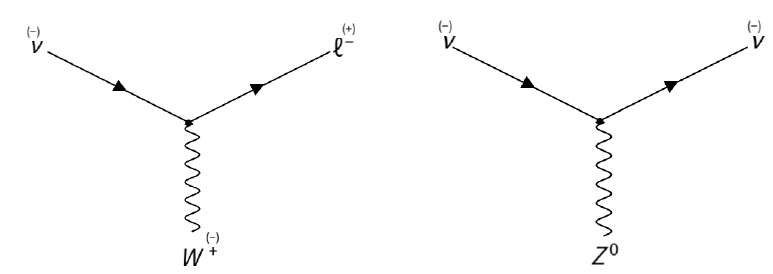
\includegraphics[width=\textwidth]{Figures/CC_NC.png}
    \caption{Feynman diagrams of charged-current (left) and neutral-current (right) neutrino interactions}
    \label{fig:CC_NC}
\end{figure}

There are multiple types of neutrino-nucleus interactions that occur which can be either charged current or neutral current interactions, or both. 

One such interaction, and often the simplest interaction is elastic scattering ($$
\nu+e^{-} \rightarrow \nu+e^{-}
$$), which occurs when a neutrino scatters off an electron with a virtual vector boson being exchanged. This type of scattering is used in the detection of low energy neutrinos, primarily those from the sun. Figure \ref{fig:elastic_scattering} shows the Feynman diagrams for this kind of interaction.

\begin{figure}
    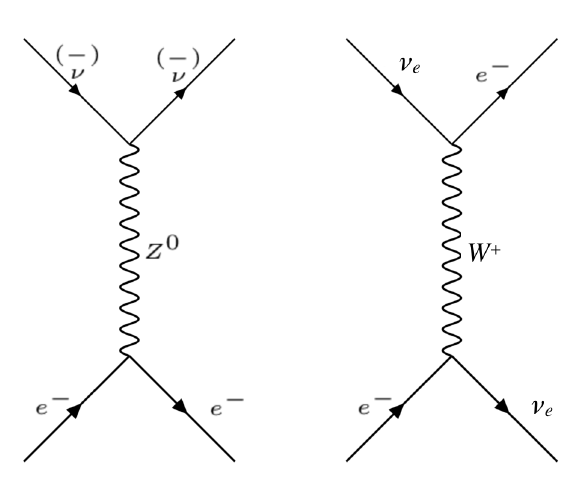
\includegraphics[width=\textwidth]{Figures/elastic_scattering.png}
    \caption{Feynman diagrams of neutral-current (left) and charged-current (right) neutrino-electron scattering}
    \label{fig:elastic_scattering}
\end{figure}

Single mesons can also be produced via neutrino-nucleon reactions: these are mostly pions, but also some kaons and eta particles can also be produced. Here a neutrino with a high enough energy, interacts with and excites a nucleon, producing a resonant baryon which decays to a nucleon and a single pion (shown in Equation \ref{eq:resonant_pion}), where $N$ and $N'$ are nucleons.

$$
\begin{gathered}
\nu_{l}+N \rightarrow l+N^{*} \\
N^{*} \rightarrow \pi+N^{\prime}
\end{gathered}
\label{eq:resonant_pion}
$$

The resonant baryon produced during the reaction is usually a $\Delta(1232)$ resonance. 

Single pion final sates can also be priduced by a neutrino which scatters an entire nucleus (X), shown in Equation \ref{eq:single_pion_CC} for the charged current reactions and Equation \ref{eq:single_pion_NC} for neutral current reactions. 

\begin{equation}
\nu_{l}+X \rightarrow l^{-}+X+\pi^{+}, \quad \bar{\nu}_{l}+X \rightarrow l^{+}+X+\pi^{-}
\label{eq:single_pion_CC}
\end{equation}

\begin{equation}
\nu_{l}+X \rightarrow \nu_{l}+X+\pi^{0}, \quad \bar{\nu}_{l}+X \rightarrow \bar{\nu}_{l}+X+\pi^{0}
\label{eq:single_pion_NC}
\end{equation}

At higher energies (above 1 GeV), neutrino interactions can also produce kaons in the final state, due to the higher energies being able to produce strange quarks. 

Deep inelastic scattering is a type of neutrino interaction where the neutrino scatters off a quark inside the proton or neutron involved in the exchange, via a W (CC) or Z (NC) boson (Equation \ref{eq:DIS_eq}), shown in Figure \ref{fig:CC_DIS}.

$$
\begin{aligned}
&\nu_{l}+N \rightarrow l^{-}+X, \quad \bar{\nu}_{l}+N \rightarrow l^{+}+X(\mathrm{CC}) \\
&\nu_{l}+N \rightarrow \nu_{l}+X, \quad \bar{\nu}_{l}+N \rightarrow \bar{\nu}_{l}+X(\mathrm{NC})
\end{aligned}
\label{eq:DIS_eq}
$$

\begin{figure}
    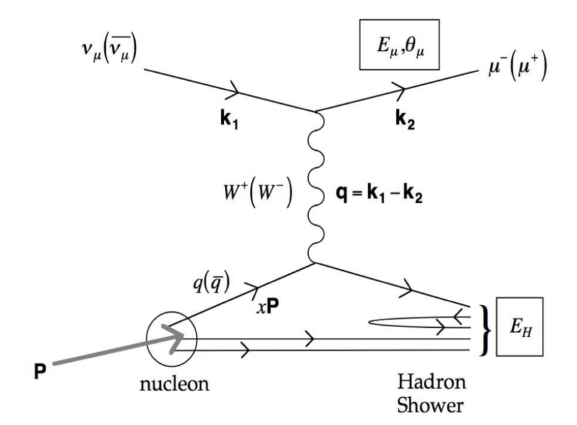
\includegraphics[width=\textwidth]{Figures/CC_DIS.png}
    \caption{Feynman diagram for a charged current deep inelastic scattering interaction with an incoming muon neutrino}
    \label{fig:CC_DIS}
\end{figure}


The next two neutrino-nucleus interactions explained here are of particular relevance to the analysis in this thesis: inverse beta decay (IBD) and quasi-elastic scattering. 

Inverse beta decay is the reaction by which Cowan and Reines first detected electron antineutrinos: it is important at low energies: from the minimum energy for the reaction to take place ($E_{\nu}$ = 1.806 MeV) to tens of MeV. Diffuse Supernova Neutrino Background and low energy antineutrinos produced from nuclear reactors can be detected via this process. Figure \ref{fig:IBD_feynman} shows the Feynman diagram for this reaction. The neutron produced by this reaction is integral to the motivation behind the Gadolinium-doping upgrade to Super-Kamiokande, which will be explained in the next section.

Finally, we get to the type of interaction investigated in this thesis: quasi-elastic scattering. This makes up the majority of the neutrino-nucleus interaction cross-sections at the energy range from 100 MeV to ~2 Gev, and therefore vital for the study of neutrinos from long baseline neutrino experiments and also low energy atmospheric neutrinos. Equation \ref{eq:QE_reaction} shows the equations for both the charge current (CCQE) and neutral current (NCQE) version of this interaction where the incoming neutrino scatters off a nucleon.

$$
\begin{aligned}
\mathrm{CC}: \nu(k)+n(p) & \rightarrow l^{-}\left(k^{\prime}\right)+p\left(p^{\prime}\right) \\
\bar{\nu}(k)+p(p) & \rightarrow l^{+}\left(k^{\prime}\right)+n\left(p^{\prime}\right) \\
\mathrm{NC}: \nu(k)+N(p) & \rightarrow \quad \nu\left(k^{\prime}\right)+N\left(p^{\prime}\right) \\
\bar{\nu}(k)+N(p) & \rightarrow \bar{\nu}\left(k^{\prime}\right)+N\left(p^{\prime}\right)
\end{aligned}
\label{eq:QE_reaction}
$$

\begin{figure}
    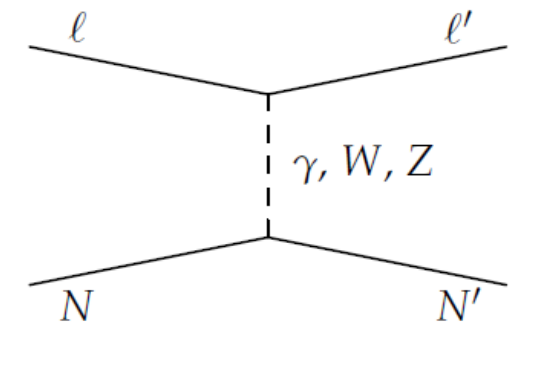
\includegraphics[width=\textwidth]{Figures/QE_feynman.png}
    \caption{Feynman diagram for a quasi elastic scattering interaction off a nucleon}
    \label{fig:QE_reaction}
\end{figure}


\subsection{Supernova Relic Neutrinos}

A key feature of the analysis presented in this thesis is that it is an investigation into the significant background of the signal for SRN. It is therefore important to state and understand the process behind the production of supernova relic neutrinos in order to get a firm handle on the motivation behind this analysis. 

\subsubsection{Supernovae Classification}
Supernovae occur when a star with a mass around eight times the mass of our sun exploads, and in a galaxy these occur only a few times in a century. Supernovae are classified into different types: Type 1a, Type 1b, Type 1c anf Type II. The classification of supernovae are determined by looking at the spectral lines in the light emitted from these supernovae. Table \ref{table:supernova_classification} shows how these supernovae are classed and which spectral line elements are associated with each class. 

\begin{center}
\begin{tabular}{||c c||} 
    \hline
    Supernova Classification & Element lines present in spectra \\ 
    \hline \hline
    Type 1a & No hydrogen, silicon  \\ 
    \hline
    Type 1b & No hydrogen, no silicon, helium  \\
    \hline
    Type 1c & No hydrogen, no silicon, no helium  \\
    \hline
    Type II & Hydrogen  \\
    \hline \hline
\end{tabular}
\end{center}

The kinetic energy of a supernova is ~$10^{44}$ J, and 99 \% of the energy from core-collapse supernovae (CCSN) are released in the the form of neutrinos. Unline Type 1a supernovae which are usually thermonuclear supernovae, Type 1b, Type 1c and Type II are core-collapse supernovae, from which more neutrinos are emitted which is why these types of supernovae are of more interest. 

\subsubsection{Core-Collapse Supernovae Mechanism}

Using the pressure produced by the process of nuclear fusion, a star is able to support itself against gravotational collapse. During the proton-proton chain reaction, hydrogen will fuse to produce helium and once temperatures and pressures are high enough, helium fusion will occur. AFter all the helium in the core is used up in the fusion process, the star will contract until the pressure and temperatures get even higher, allowing more massive nuclei to fuse. This reaction will carry on until iron nuclei are produced, this being the element with the highest binding energy, causing the fusion to stop.
\newline
As more and more iron accumulates in the core of the star. the density and temperature of the core will increase, and these higher energy electrons will increase the rate of electron capture on protons that will occur in the iron nuclei. This will cause a reduction in the electron degeneracy pressure, which is further enhanced by the breakdown of the iron nuclei which occurs at higher temperatues when gamma rays interact with them. The degeneracy pressure is no longer greater than the gravitational forces acting inwards, and gravitational core collapse occurs. The point at which in the core the neutrino mean free paths become become approximately the same size as the proto-neutron star is called the "neutrinosphere".  The radius of the neutrinosphere becomes as large as that of the inner core of the star, when the inner core of the star reaches a density of ~$10^{11} gcm^{-3}$, and the electron neutrinos produced from electron capture become unable to escape. Gravitational collapse of the star continues until the inner core reaches nuclear density, at which point a shock wave is produced due to the repulsive force between nuclei. When this shock wave reaches the neutrinosphere, neutrino emission begins, which lasts less than 10 milliseconds. After this shockwave passes, nucleons and electrons fall back onto the proto-neutron star which heats it up. This causes neutrinos of all flavours to be produced via pair production and electron capture. This is called the "accretion phase". Due to this expulsion of neutrinos the shock wave loses energy, but it is revived through matter behind the shock wave being heated by neutrino absorption from the proto neutron star region. After the shock wave is revived, if it has enough energy to blow off the outer layer of matter a supernova occurs. Then, depending on the mass of the PNS, it cools to either become a neutron star or a black hole. If the shock wave energy is not high enough to blow off the outer layer of matter, the accretion phase continues until a black hole is formed.

The energy of the emitted neutrinos depend on their flavour - neutrinos emitted from a deeper layer inside the supernova will be higher in temperature and therefore have a higher energy. For electron neutrinos and electron anti-neutrinos. the dominant interactions are charged current interactions with nucleons. Due to the number of neutrons in a proto-neutron star greatly outnumbering the number of protons, the interaction involving $\nu_{e}$ will be far more efficient than those involving $\nu_{\bar{e}}$, meaning the neutrinosphere for $\nu_{\bar{e}}$ is smaller than for $\nu_{e}$, so they are emitted from the PNS with greater energies. 

Due to there being no charged current interactions involving muon neutrinos in the medium, they involved instead in neutral current reactions, including Bremsstrahlung, neutrino-pair annhilation, and electron-positron pair annhilation. Due to only undergoing these reactions their neutrinosphere is even smaller than that of their electron neutrino and electron anti-neutrino counterparts, therefore being emitted wih even higher energies. \cite{nagakuraNonthermalNeutrinosCreated2021}. Figure \ref{fig:ccsn_nu_flavor_energy} shows the luminosity (top panels) and average energy (bottom panels) for three different neutrino flavours as a function of time for the neutronisation phase (left), accretion phase (centre) and cooling phase (right). Taken from \cite{chakrabortyObservingSupernovaNeutrino2014}.

Kamiokande-II observed neutrinos produced from a supernova, later named 1987A in the Large Magellenic Cloud. These neutrinos were also observed by the Irvine-Michigan-Brookhaven detector and the Baskan Neutrino Observatory.






\subsection{Analysis Motivation}






 %   \part{NEUTRINOS \& SUPERNOVAE}
  \chapter{The Tokai-to-Kamioka experiment}
\label{chp:t2kdetector}

The Tokai-to-Kamioka (T2K) experiment is a long baseline neutrino oscillation experiment based in Japan and its purpose is to study neutrino oscillations: specifically a precision measurement of the neutrino oscillation parameters $\Delta m_{23}^{2}$ and $\sin ^{2} \theta_{23}$ and to increase the measurement to the leptonic CP violating phase $\delta_{CP}$, which are mentioned in Chapter 1. The experiment produces a beam of intense muon neutrinos at J-PARC (Japan Proton Accelerator Research Complex) in Tokai, which is located on the far east coast of Japan in Ibaraki Prefecture. The muon neutrino beam travels 295 km west towards the far detector Super-Kamiokande (see Chapter 3.)  These neutrinos are detected by other detectors such as ND280 and INGRID, before they oscillate and reach Super-Kamiokande which is important with regards to measuring the neutrino oscillation parameters. ND280 and Super-Kamiokande are off-axis detectors, meaning that they are placed 2.5$\degree$ off axis to the centre of the neutrino beam - this allows for the peak of the energy of the muon neutrinos to be at 0.6 GeV, meaning that the neutrino oscillation on the 295 km baseline is maximised, and the reduced spread in muon neutrino energy means that these detectors are far less susceptible to potential backgrounds. This chapter explains production of the muon neutrino beam from the JPARC proton beam line and the near detector complex.

\subsection{Neutrino beam production}

\subsubsection{JPARC proton beam production}

The production of a proton beam from JPARC is due to three accelerators, the LINAC (linear accelerator), an RCS (rapid cyclic synchrotron) and the main ring synchrotron (MR). A negative hydrogen ion is accelerated to a kinetic energy of 400 MeV, from which a beam of protons is created by converting the negative hydrogen ion beam using charge-stripping foils. This proton beam is then accelerated to a kinetic energy of 3 GeV by the RCS, and about 5\% of the bunches produced from this process are passed to the MR where the proton beam will be accelerated up to 30 GeV. 

\subsubsection{Neutrino beam production}

The neutrino beam is produced using a primary and a secondary beamline as shown in Figure \ref{fig:nubeamline}. The primary beamline involves taking the proton beam from the MR and targeting it towards the direction of Kamioka and then transferring it through a succession of beam monitors which measure facets of the neutrino beam including the beam profile, intensity and position. The beam monitor which is closest to the graphite target measures the "Protons-On-Target" (POT), a value used to determine the neutrino beam flux. The secondary beamline involves taking the proton bunches and passing them through a target station, the decay volume and the beam dump. After interacting with the target station, the proton bunches are collimated through a 1.7 m graphite rod where the collimated hole the proton bunches pass through are 30 mm in diameter. Beam profile reconstruction occurs in the OTR (Optical Transition Radiation) monitor, made up of titanium alloy foil placed at a 45 degree angle in order to intercept the beam. As the proton beam enters the foil, the visible light that is produced escapes through a collection of mirrors and is then captured by a charge injection device camera, which creates the beam profile. After beam profiling, the proton beam then impacts upon a graphite rod target which is 91.4 cm long and 2.6 cm in diameter - this collision produces secondary hadrons, including pions which are focused by three magnetic horns. These magnetic horns can be used to produce either a muon neutrino or muon antineutrino beam depending on the polarity of the 250kA current they are pulsed with. If a +250 kA current is used, the positive pions and kaons produced can go on to make muon neutrino beams wheareas if a -250 kA current is used negative pions and kaons can decay to create muon antineutrino beams (both are shown in Equation \ref{eq:nubeam}). The +250 kA mode is called Forward Horn Current (FHC) mode and the -250 kA mode is called Reversed Horn Current (RHC) mode, and the analysis in this thesis will occur in FHC mode only. 

\begin{equation}
\begin{array}{lll}
\pi^{+} & \longrightarrow \mu^{+}+\nu_{\mu} & \text { FHC } \\
\pi^{-} & \longrightarrow \mu^{-}+\overline{\nu_{\mu}} & \text { RHC }
\end{array}
\label{eq:nubeam}
\end{equation}

A 75 ton volume beam dump made of graphite and iron stops the particles, specifically the protons, secondary hadrons and mesons which have a momentum below 5 GeV/c end up being absorbed by the beam dump. A muon monitor is placed after the beam dump in order to directly measure the the beam intensity and beam direction - muons can be used to monitor the beam properties because along with the neutrinos these are the main particles produced from the pion decay. After the muon monitor, a nucleon emulsion plate detector measures the flux and momentum of the muons. 

\subsection{Near detectors}

\subsubsection{ND280}

ND280 is a near detector which sits 280 m from the graphite target. It is an off-axis detector, meaning that just like Super-Kamiokande, it is placed 2.5 $\degree$ off-axis from the center of the beam. This stems from the relationship between the energy of the neutrinos produced from the decay of the pions, a relationship shown in Equation \ref{eq:piondecay}. 

\begin{equation}
    E_{\nu}=\frac{m_{\pi}^{2}-m_{\mu}^{2}}{2\left(E_{\pi}-\sqrt{E_{\pi}^{2}-m_{\pi}^{2}} \cos \theta\right)}
\label{eq:piondecay}
\end{equation}

where $E_{\pi}$ is the energy of the parent pion and $\theta$ is the scattering angle between the direction of the outgoing neutrino and the direction of the parent pion's momentum. $m_{pi}$ is the parent pion mass and $m_{\mu}$ is the mass of the outgoing muon. Figure \ref{fig:energyangle} shows the neutrino energy from pion decay plotted against the energy of the parent pion for a range of off-axis angles. 

\begin{figure}
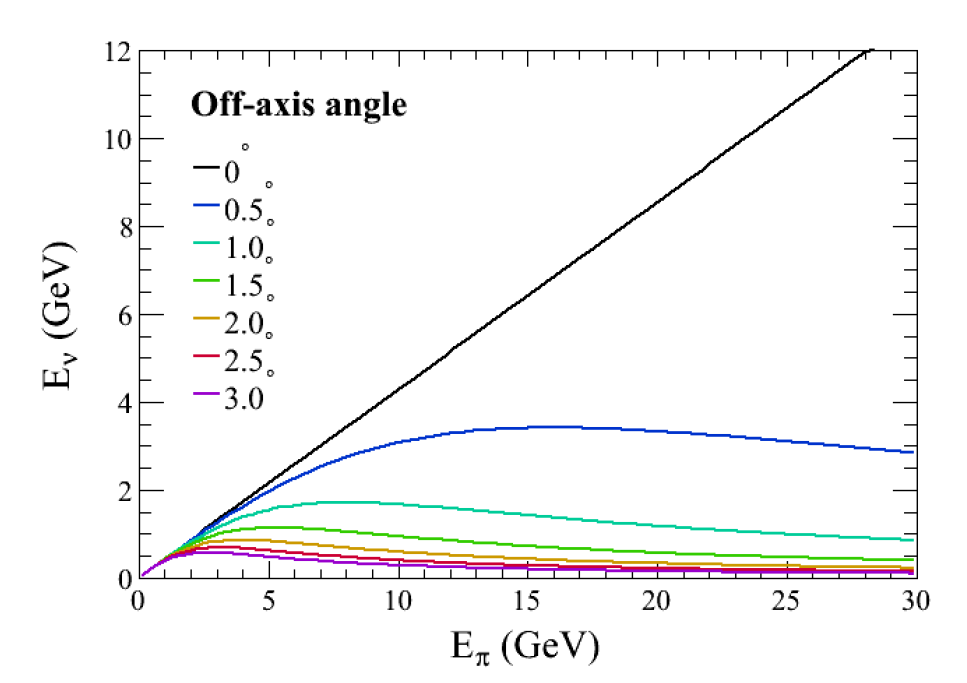
\includegraphics[width=\textwidth]{Figures/energyangle.png}
\caption{Energy of the neutrino plotted against the energy of the parent pion for multiple different off-axis angles}
    \label{fig:energyangle}
\end{figure}

As off-axis angle increases, the intensity of the neutrino beam decreases, and therefore picking an off-axis angle of 2.5 $\degree$ at which to place the ND280 detector complex strikes a good balance between keeping a high beam intensity while ensuring a peak energy of 0.6 GeV in order to have the neutrino oscillation be maximised at 295km. The relationship between muon neutrino oscillation probability and muon neutrino energy is shown at the top in Figure \ref{fig:nuprobosc}, and at the bottom the muon neutrino flux 295 km away from the graphite target can be seen for three different off-axis angles.

\begin{figure}
    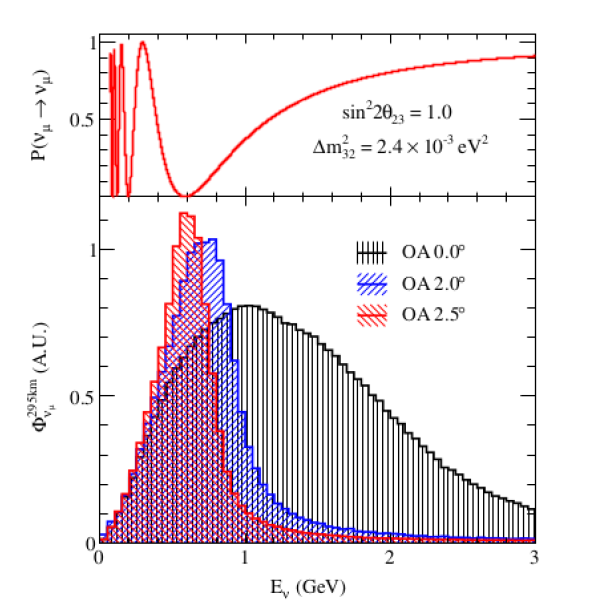
\includegraphics[width=\textwidth]{Figures/nuprobosc.png}
    \caption{The probability of survival of muon neutrinos (top plot) and neutrino beam flux at the 295km far detector (bottom) Taken from \cite{t2kcollaborationT2KNeutrinoFlux2013}.}
    \label{fig:nuprobosc}
\end{figure}

Figure \ref{fig:ND280_schematic} shows a schematic of the ND280 detector complex. It has three main goals: firstly, to measure the cross sections of muon neutrino interactions, so neutrino-nucleus interaction models can reduce their systematic uncertainties. Secondly, measuring the component of the neutrino beam which is made of electron neutrinos, hence being able to better constrain the background to electron neutrino appearance at the far detector. And thirdly, to determine the event rate at Super-Kamiokande by measuring the energy spectrum of the muon neutrinos produced. 

\begin{figure}
    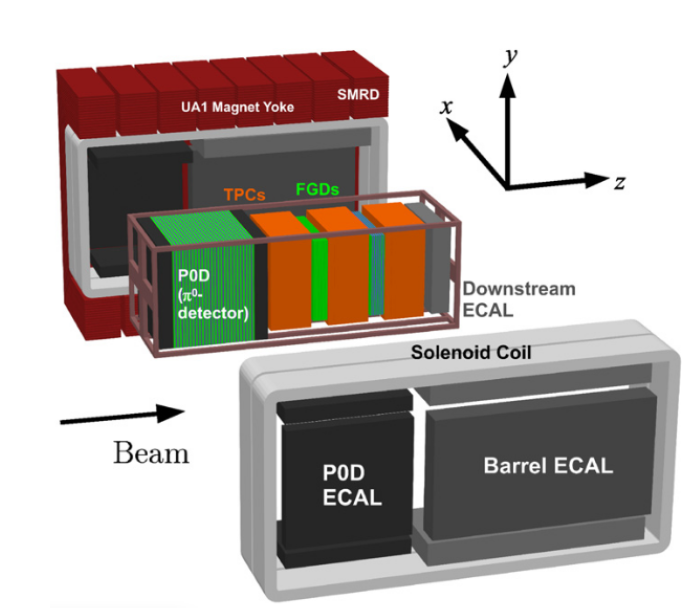
\includegraphics[width=\textwidth]{Figures/nd280_complex.png}
    \caption{Near detector ND280 schematic taken from \cite{t2kcollaborationT2KExperiment2011}.}
    \label{fig:ND280_schematic}
\end{figure}

N2D280 is made of a neutral pion detector ($P0D$), three Time Projection Chambers (TPCs) and two Fine Grained Detectors (FGDs). These are enclosed within Electromagentic Calorimeters (ECals) and a Side Muon Range Detector (SMRD). These detectors are magnetised using a magnet (UA1). 

The neutral pion detector is important due to its ability to detect a process that can imitate the important signal event of electron neutrino appearance at Super-Kamiokande. Neutral pions are produced during the neutral current interactions on water ($\nu_{\mu} + N \rightarrow \nu_{mu} + N +\pi^{0} + X$) and the purpose of $P0D$ is to measure the cross-section of this interaction. The central part of the $P0D$ detector is made of planes of scintillator, brass and water bags which are placed in alternating layers as shown in Figure \ref{fig:p0d}. There are also two electromagnetic calorimeters which remove events entering the detector from the outside.  Each scintillator plane is made of hollow triangular scintillator bars containting wavelength shifting fibres (WLS) which collect the charged particles which pass through the bars and transport them to multi-pixel photon counters (MPPCs). The electromagnetic calorimeters (ECal) are placed around the neutral pion detector, the time projection chamber-fine grain detector tracker and downstream of the last time projection chamber. These ECal can detect photons when they are surrounding the neutral pion detector and the downstream calorimeter can aid in the 3D reconstruction of the charged particle tracks. The SMRD (Side Muon Range Detector) is used as a way to measure the momenta of muons which escape the detector complex at a large ange relative to the direction of the beam.

\subsubsection{INGRID detector}

The INGRID (Ineractive Neutrino GRID) detector is a neutrino detector which unlike ND280 is placed on-axis instead of off-axis. This allows it to directly monitor the direction of the neutrino beam and the intensity of the neutrino beam by measuring the interactions of the neutrinos with the alternating iron that make it up. INGRID is also placed 280 m from the graphite target and consists of 14 modules placed in a cross formation, with the centre of the cross placed at the centre of the neutrino beam. The INGRID modules are comprised of nine iron plates alternating with 11 tracking scintillator planes, which are themselves surrounded by scintillator plates the purpose of which is to reject interactions that occur outside the module. A schematic of the INGRID cross is shown in \ref{Fig:ingridcross} and a schematic of the modules is shown in \ref{Fig:ingridmodule}. 

\begin{figure}
    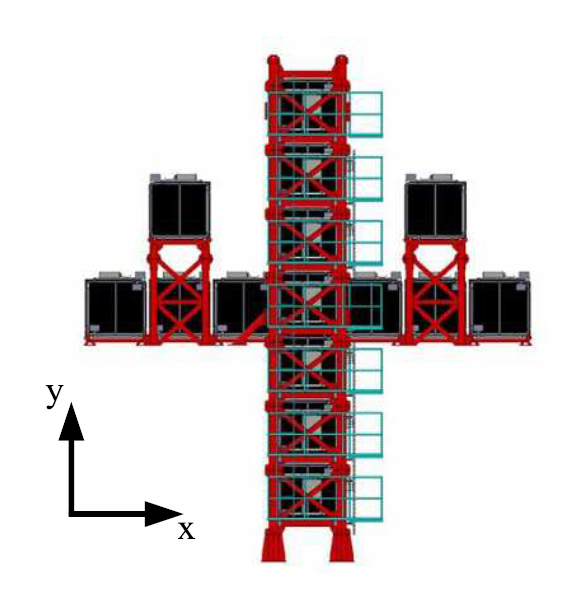
\includegraphics[width=\textwidth]{Figures/ingridcross.png}
    \caption{Schematic of the INGRID cross taken from \cite{t2kcollaborationT2KExperiment2011}.}
    \label{fig:ingridcross}
\end{figure}
\begin{figure}
    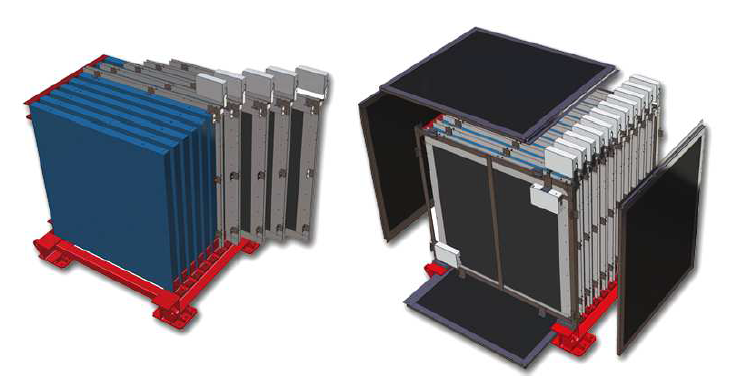
\includegraphics[width=\textwidth]{Figures/ingridmodule.png}
    \caption{Individual INGRID module schematic taken from \cite{t2kcollaborationT2KExperiment2011}.}
    \label{fig:ND280_schematic}
\end{figure}

An additional module, called the proton module was added to measure the muons in combination with protons produced by the neutrino beam in INGRID. This module is used to distinguish the quasi-elastic interaction channel in order to compare it with Monte Carlo simulations of the beamline and neutrino interactions. The Proton Module is made of scintillator planes (no alternating iron plates) and is contained by veto planes. The Proton Module was placed in the centre of the INGRID cross at the intersection of the vertical and horizontal modules. Figure \ref{fig:ingridevent} shows what a standard neutrino event looks like inside the INGRID module. A neutrino enters from the left and after interacting with the scintillator cells (shown in green) produces a tracks (shown in red), with the relative size of each circle corresponding to the observed signal in that cell. The blue cells show the position of the veto scintillators, while the gray planes show the iron plates. 
  \chapter{The Super Kamiokande Detector}
\label{chp:superk}



\section{The Super-Kamiokande detector}

\subsection{Background and detector design}

Super-Kamiokande is a neutrino observatory consisting of a cyclindrical tank which is 41.4 m in height and 39.3 m in diamter, and filled with 50kton of ultrapure water and gadolinium sulphate. It is used as a neutrino detctor for atmospheric, solar and astrophysical neutrinos, as well as being a far detector of the Tokai-to-Kamioka neutrino beam. It is based in the Mozumi mine, located in Gifu Prefecture, Japan. Due to it's location being underneath Mount Ikenoyama, 1000m underground, it is shielded as much as possible from the cosmic ray muon detector background. Super-Kamiokande is divided into two concentric cylinder volumes, consisting of the inner detector (ID) and outer detector (OD) using a stainless steel structure which supports the photomultiplier tubes. Tyvek and black polyethylene terephthelate sheets are mounted on this structure in order to optically seperate the inner and outer detector \cite{suzuki_super-kamiokande_2019}.

The inner detector is a cylinder which has a diameter of 33.8 m and a height of 36.2m, and has a fiducial volume of 22.5 ktons of water. The fiducial volume is defined as the region inside a surface drawn 2.00 m from the inner detector wall: using this fiducial volume gives protection against events produced from natural radioactivity in the surrounding rock. It is host to 11,129 photomultiplier tubes which give 40\% photocoverage of its inner surface, with the specific photomultiplier model chosen being the hemispherical, 50.8 cm diameter Hamamastu R3600 model. The 2 m wide outer detector has only 1885 photomultiplier tubes which are mounted on the outside of stainless steel structure, each with a smaller diameter of 20cm, and are either the R1408 or R5912 Hamamatsu model. Each outer detector photomultiplier tube is attached to a 50cm x 50cm wavelength shifting plate, improving the light collection ability in the OD \cite{fukuda_super-kamiokande_2003}.

A detailed schematic of the photomultiplier tubes used in Super-Kamiokande can be seen in Figure \ref{fig:PMTdiagram}. The photocathodes used in these PMTs are comprised of bialkali antimony-potassium-caesium material (Sb-K-Cs), which give a greater sensitivity on to longer wavelengths, giving the greatest spectral response at 360 nm, near the ultraviolet range. This makes these types of photocathodes suitable to use for matching with light sources in the blue region of the visible spectrum, which is the region in which the wavelength of Cherenko photons lie. The 11 dynodes which are inside the photomultiplier tube are arranged in a "venetian blind" fashion, meaning that the dynodes consist of an assembly of parallel strips. This results in a good collection efficiency of the multiplied electrons and gives decent protection from external magentic fields. More protection from external magnetic fields is provided by a set of Helmholtz coils which are aligned outside the innter detector, which reduce the ambient background geomagnetic field from 450mG to 50mG. This is needed due to the systematic bias that could occur due to the strength and uniform direction of the geomagnetic field affecting the photo-electron trajectories and consequently the photomultiplier tube hit timing. 

\begin{figure}
    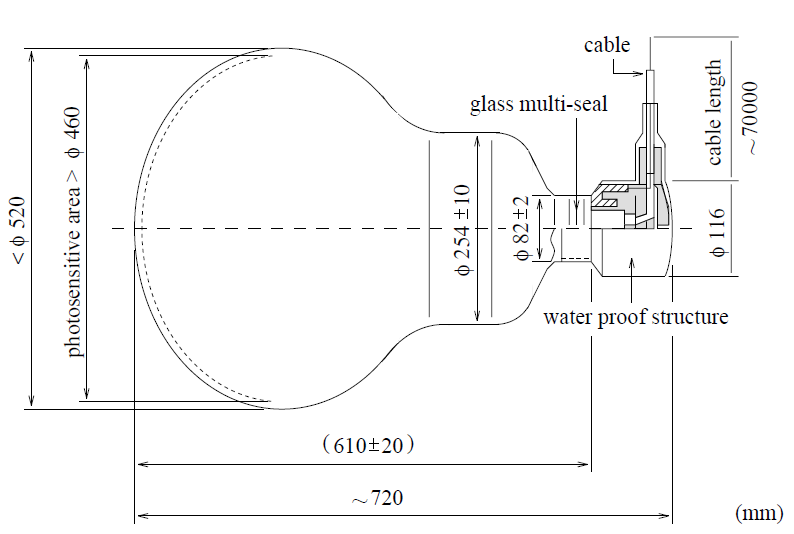
\includegraphics[width=\textwidth]{Figures/PMT_schematic.png}
\caption{Schematic of an ID 50 cm Super-Kamiokande PMT \cite{fukuda_super-kamiokande_2003}.}
    \label{fig:PMTdiagram}
\end{figure}


Radioactivity from radon, uranium and thorium radioisotopes in the Super-Kamiokande tank water and radon in the surrounding air could provide a low energy background to measurements which should be negated. In low-energy analyses, such as the analysis in this thesis, this becomes an even more significant issue. Microbes present in the mine water also present a problem as they cause a reduction in the value of the light attenuation length by a factor of 2.72. Therefore the water used in Super-Kamiokande has to undergo a purification process - the water used is continuously reprocessed at a rate of 30 tons $h^-1$ in a closed loop system, which is the same method used to purify the water when refilling the tank. The first step of this water purification process is to use a 1$\micro m$ mesh filter to remove large particulates of impurities from the water. \cite{fernandez_status_2016}.A heat exchanger is then used to cool down the water to a constant 13.0 \degree C to reduce the dark noise hits of the photomultiplier tubes and the growth of the microbes. A treatment with ultraviolet light is then used to kill any remaining microbes in the water. Radon-free air is then dissolved into the water to aid in the later process of radon removal from the water and a high performance membrane ultra filter (UF) is used to remove organic compounds about 10 nm in diamater from the water. After this step a membrane degasifier removes the dissolved radon, where 30 L of radon reduced air is supplied to the membrane degasifier. The dissolved radon will transfer across the membrane but the water will not, allowing for efficient radon reduction. The inner detector tank water is circulated by injecting the water at the bottom of the tank and exctracting it from the top, where the convection currents are able to maintain the temperature in the region within 11m to the bottom of tank, however, outside this region the present temperature gradient causes an asymmetry in the attenuation of light, which is discussed more in Chapter 3. 
\newline
 An air purification system is also installed in Super-Kamiokande in order to reduce the amount of Radon present which could dissolve into the tank and affect measurements. The level of radon activity achieved after this air purification has taken place is 1 mBq/$m^{3}$.

The Super-Kamiokande experiment began taking data on 1st April 1996, and due to maintenance was shut down in July 2001, which was phase I of the experiment. A table of the Super-Kamiokande phases is shown in Table \ref{table:phasetable}. During the refilling of the tank after maintenence, there was cascade of PMT implosions that occurred on the 12th of November 2001, which were triggered by the implosion of a single photomultiplier tube, due to a microfracture in the neck of the tube. This implosion destroyed about 7,000 of the PMTs and in order to avoid such chain reactions in the future, from 2002 onwards all of the inner detector PMTs were fitted with acrylic covers and fiber-glass reinforced plastic (FRP) cases. Detector shutdown and rebuild took nine months and Super-Kamiokande resumed data taking with the full number of photomultiplier tubes in July 2006 which marked the beginning of Super-Kamiokande phase III. Super-Kamiokande phase IV began in September 2008 where a new data aquisition system and charge to time (QTC) based electronics with Ethernet (QBEE) was deployed in order to measure arrival times and integrated charge for inner detector and outer detector photomultiplier tube signals. This replaced the ATM (Analogue and Timing Module) which was used in Phase I, II and III of Super-Kamiokande. The improvements in electronics and calibration methods meant that when Super-Kamiokande phase IV started running in September of 2008, electrons with energies as low as 3.5 MeV were able to be detected.

\begin{table}[htp]
    \centering
    $$
\begin{array}{|c|c|c|c|c|c|}
    \hline \multirow{2}{*}{\text { Phase }} & \multirow{2}{*}{\text { Phase Period }} & \multicolumn{2}{|c|}{\text { Total PMT number  }} & \multirow{2}{*}{\text { FRP case? }} & \multirow{2}{*}{\text { Electronic type }} \tabularnewline
    \cline {3-4} & &  \text { ID (Coverage) } & \text { OD } & & \tabularnewline
    \hline \hline \text { SK-I } & \text { Apr. 1996 - Jul. 2001 } & 11146(40 \%) & 1884 & \text { no } & \text { ATM } \\
    \hline \text { SK-II } & \text { Oct. 2002 - Oct. 2005 } & 5182(19 \%) & 1884 & \text { yes } & \text { ATM } \\
    \hline \text { SK-III } & \text { Jul. 2006 - Sep. 2008 } & 11129(40 \%) & 1884 & \text { yes } & \text { ATM } \\
    \hline \text { SK-IV } & \text { Sep. 2008 - Today } & 11129(40 \%) & 1884 & \text { yes } & \text { QBEE } \\
    \hline \text {SK-V}    &  \text{} &  11129(40 \%) & 1884 & \text { yes } & \text { QBEE } \\
\end{array}
    $$
\caption{Phases of Super-Kamiokande and main properties of each phase }
\label{table:phasetable}
\end{table}



\subsection{Data aquisition system}

As shown in Table \ref{table:phasetable}, Phase IV of the experiment marked the beginning of Super-Kamiokande using QTC-based Electronics with Ethernet (QBEEs). Each QBEE board used in Super-Kamiokande contains 24 photomultiplier tube input channel, where each channel uses a charge-to-time (QTC) converter and a time-to-digital converter placed in series as shown in Figure \ref{fig:superkdaq}. After a single photoelectron is produced by the photomultiplier tubes after incident photons have been recieved upon it, the dynodes inside the photomultiplier tube amplify this photoelectron so that each photoelectron that strikes the surface of the dynode produces several more photoelectrons, which are produced from the dynodes as an analogue signal. This signal then enters a charge-to-time converter (QTC), an application specific integrated circuit (ASIC) which was specifically designed for Super-Kamiokande in order to detect photomultiplier tube signals using built-in discriminators and to produce output timing signals whose widths represent the integrated charge of the PMT signal. The QTC used has three input channels per chip, which has three gain ranges (Small, Medium, Large as shown in Figure \ref{fig:superkdaq}). There is a built in discriminator inside the QTC which determines whether the the signal from a PMT is a "hit". If the PMT signal exceeds the threshold value of this discriminator, the QTC integrates the charge of the signal over the next 400ns, and a square wave pulse is generated whose pulse width is proportional to the intergrated charge of the input signal from the PMT. The next ~400ns is used to discharge the integrated charge from the QTC, leading to a total channel dead time of 900 ns due to summing the charge integration and discharge of the QTC. 
\newline

\begin{figure}
    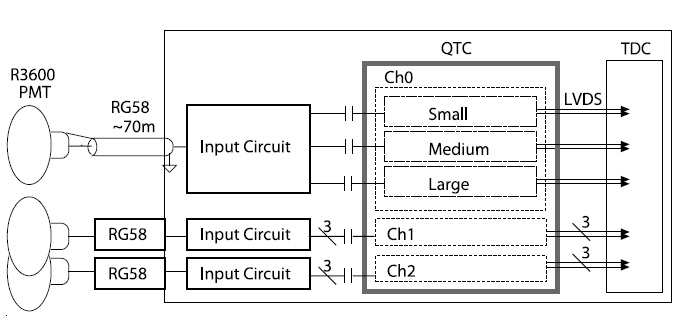
\includegraphics[width=\textwidth]{Figures/superk_daq.png}
\caption{Schematic of the charge-to-time converter circuit \cite{nishino_high-speed_2009}.}
    \label{fig:superkdaq}
\end{figure}

A time-to-digital converter (TDC) then digitises the output time signal, so the PMT charge information is retained. These digitised outputs are collated by 20 front-end computers which collects all the information from the inner and outer detectors, with each computer taking the PMT hit information from 30 inner detector and 20 outer detector QBEE boards and sorting the PMT hit time information in order of the raw hit time. This information is then sent to "merger" computers, who then produce a full time-ordered list of all PMT hits. These merger computers then apply software triggers to select event candidates, using $N_{200}$, a quantity which determines the number of PMT hits in a 200 ns timing window. When the value of $N_{200}$ surpasses the threshold value of a certain trigger type (whether it is a SLE (Super Low Energy), LE (Low Energy), HE (High Energy), SHE (Super High Energy), OD (Outer Detector) or AFT (After Window) trigger), the trigger is used to select an event candidate. The SLE, LE, HE and SHE triggers roughly define the energy of a certain event, based on the number of hits detected. The OD trigger is used to veto events, and the AFT trigger is of special importance to the analysis in this thesis: it is used to discern when a neutron is produced after a neutrino interaction. The AFT Trigger is issued to take 500 $\mu$sec of data after SHE trigger in order to identify the positron from the prompt event and the delayed 2.2 MeV gamma released from the neutron capture on the proton during the IBD reaction. Another set of computers acts as an "organiser": it takes all the information regarding the event candidates from the "merger" computers and writes them onto disks \cite{fukuda_super-kamiokande_2003}.


\section{Event Reconstruction}

\subsection{Vertex Reconstruction}
For low energy events (events up to 100MeV), Super-Kamiokande currently uses BONSAI (Branch Optimisation Navigating Successive Annealing Interactions) for event reconstruction. Vertex reconstruction for Super-Kamiokande has undergone changes and improvements depending on the phase of the experiment. 
\newline{}
For Phase I of Super-Kamiokande, vertex reconstruction depended on a lattice of test vertices with 4m spacing throughout the detector, with a specific measure of goodness for each test vertex: the test vertex with the highest measure of goodness would have around it a more finely spaced grid, and the process would be repeated. For Phase II of Super-Kamiokande due to the reduced number of PMTs, this approach was no longer as successful as it was in Phase I and as a result the reconstruction perfomance declined, and BONSAI was created as a replacement. Instead of using a fixed grid which was the case with SK-I and SK-II, BONSAI creates test vertices by selecting groups of four PMT hits and seeing where the timing residuals of the PMT hits would be most reduced. After these test vertices have been indentified, a maximum likelihood fit over all the PMT hits in the event is performed, shown in Equation \ref{bonsailikelihood}.

\begin{equation}
    \mathcal{L}(\vec{x}, t_{0})=\sum_{i=1}^{N_{\text {hlt }}} \log (P(t-t_{\text {tof }}-t_{0}))
\label{bonsailikelihood}
\end{equation}

where ($\vec{x}, t_{0}$) is the test vertex, and $(P(t-t_{\text {tof }}-t_{0}))$ is the probablility density function of the timing residual, which for each PMT hit is defined as $(t-t_{\text {tof }}-t_{0})$, where $t_{0}$ is the time of the interaction, $t_{tof}$ is the time of flight from the interaction vertex position to the position of the hit PMT, $t$ is the PMT hit time. The 1$\sigma$ difference between the true vertex position and the reconstructed vertex position plotted as a function of true electron energy is shown in Figure \ref{fig:bonsaivertexres}. 

\begin{figure}
    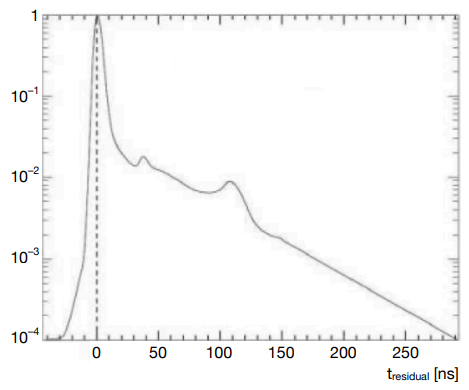
\includegraphics[width=\textwidth]{Figures/bonsai_pdf_res.png}
\caption{Probability density of the timing residual P$(t-t_{\text {tof }}-t_{0})$, where $t_{0}$ use for the vertex reconstruction maximum likelihood fit. The peaks at 30ns and 100ns are caused by PMT after-pulsing.}
    \label{fig:bonsaivertexres}
\end{figure}

\begin{figure}
    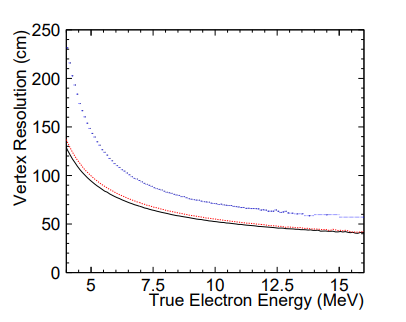
\includegraphics[width=\textwidth]{Figures/bonsai_vertex_res.png}
\caption{The vertex resolution (the point at which 68\% of the events in the distance distribution between the actual and reconstructed vertex are contained) for the different SK phases. SK-I (Blue), SK-III (Red), SK-IV (Black).}
    \label{bonsaivertexres}
\end{figure}

\subsection{Direction Reconstruction}

Cherenkov light is emitted in a conical formation as electrons and positrons travel through water, with a Cherenkov angle of $\approx 42\degree$. BONSAI can reconstruct the direction of these particles by using this information along with the reconstructed vertex. This reconstruction occurs using a maximum likelihood function defined in Equation \ref{directionlikelihoodeq}.

\begin{equation}
    \mathcal{L}(\vec{d})=\sum_{i}^{N_{20}} \log (f(\cos\theta_{i}, E))\times\frac{\cos\theta_{i}}{a(\theta_{i})}
    \label{directionlikelihoodeq}
\end{equation}

$f(\cos\theta_{i},E)$ is the expected distribution of the angle between the vector of the direction $\vec{d}$ of the particle, and the observed Cherenkov photon from the position of the reconstructed vertex. The reason there is a spread in this energy distribution is because while the highest value of this distribution occurs at the cosine of the opening Cherenkov angle of $42\degree$, due to the particle travelling through the water being Coulomb scattered multiple times, there is a variation in the angle because of the varying particle energy. $N_{20}$ is the number of hits whose residual hit time is within 20ns of the time of the reconstructed event, which is used in order to reduce the amount dark noise and scattered photons contribute to the direction reconstruction calculation. The  variable $a(\theta_{i})$ is used in the second term in Equation \ref{directionlikelihoodeq}, and it is linked to the angle of incidence of the photon on the PMT $a(\theta_{i})$, and is a correction factor stemming from the acceptance of PMTs and therefore linked to the shape of the PMT and it's acrylic case. 


\subsection{Energy reconstruction}

The kinetic energy of a particle is proprtional to the amount of Cherenkov photons emitted from it, and if we assume that the Cherenkov photons in a single event come from a single electron, we can reconstruct the total energy of the electron. Instead of using the number of photoelectrons of all hit photomultiplier tubes to reconstruct the energy of low energy events, the number of hit photomultiplier tubes is used instead. The reasons for this are threefold - firstly, low energy events emit a small number of Cherenkov photons, and therefore average about one photon per hit PMT. Secondly, at single photoelectron level, the resolution of the PMTs are is poor, and third, the number of photoelectrons produced is related to the gain of the photomultiplier tubes, which is given by equation:

\begin{equation}
    G(i) \propto \frac{Q_{o b s}(i)}{N_{o b s}(i)}
\label{gain_equation}
\end{equation}

where $G(i)$ is the gain of each PMT and $Q_{obs}(i)$ is the average charge for each inner detector photomultiplier tube, and $N_{obs}(i)$ is the number of times that photomultiplier tube $i$ registers a charge which is greater than the threshold charge value. Due to the variation in gain value not affecting the number of hit photomultiplier tubes as much as it does for the number of photoelectrons, number of hit PMTs is used instead. Energy reconstruction uses $N_{50}$, which is the number of photomultiplier tube hits in a 50 ns window, which allows for the rejection of dark noise hits for the photomultiplier tubes. The number of effective photomultiplier tubes which are hit, the number of hit PMTs in this timing window of 50ns is summed up, while being weighted with correction factors, shown in Equation \ref{effectivePMTs} \cite{ueno_analysis_nodate}. 

\begin{equation}
    N_{e f f}=\sum_{i=1}^{N_{50}}\left[\left(X_{i}-\epsilon_{\text {dark }}+\epsilon_{\text {tail }}\right) \times \frac{N_{\text {all }}}{N_{\text {alive }}} \times \frac{1}{S\left(\theta_{i}, \phi_{i}\right)} \times \exp \left(\frac{r_{i}}{\lambda}\right) \times G(i)\right]
    \label{effectivePMTs}
\end{equation}

where $X_{i}$ is the correction factor hits with many photoelectrons. This correction factor is important because if some photomultiplier tubes are hit by multiple photons (for example, if the edge of the fiducial volume is where the event vertex took place). The number of photoelectrons produced by each hit photomultiplier tube is estimated using the occupancy of the eight photomultiplier tubes which surround it. Using the number of hit photomultiplier tubes ($n_{i}$) and the number of functional photomultiplier tubes that surround the i-th photomultiplier tube ($N_{i}$), the formula for $X_{i}$ is shown in Equation \ref{eq:correction_factor}.

\begin{equation}
    X_{i}=\left\{\begin{array}{ll}
    \log \left(1-n_{i} / N_{i}\right)^{-N_{i} / n_{i}} & \left(n_{i}<N_{i}\right) \\
    3 & \left(n_{i}=N_{i}\right)
    \end{array}\right.
    \label{eq:correction_factor}
\end{equation}


$\epsilon_{dark}$ in Equation \ref{eq:correction_factor} is a correction factor for dark noise hits, shown in Equation \ref{edark}, where $R_{dark}$ is the average value for the dark rate during the run period that the event is in and $N_{\text {PMT}\text {alive }}$ is the number of active photomultiplier tubes in the inner detector.


\begin{equation}
    \epsilon_{\text {dark }}=\frac{N_{\text {PMT}\text {alive }} \times R_{\text {dark }} \times 50 \mathrm{~ns}}{N_{50}}
    \label{edark}
\end{equation}

$\epsilon_{tail}$ is the correction factor for photomultiplier tube hits which are in the tail end of the 50ns timing window, and is defined in Equation $\ref{etail}$.

\begin{equation}
    \epsilon_{\text {tail }}=\frac{N_{100}-N_{50}-N_{\text {alive }} \times R_{\text {dark }} \times(100-50) \mathrm{ns}}{N_{50}}
    \label{etail}
\end{equation}


$\frac{1}{S(\theta_{i}, \phi_{i})}$ is the inverse of the effective area of the ith hit photomultiplier tube photocathode, from the direction of the incident photon given by $(\theta_{i}, \phi_{i})$.

$G(i)$ is the gain correction for the quantum efficiency of the photomultiplier tubes and $exp(\frac{r_{s}}{\lambda})$ is the correction for water transparency which accounts for the amount of attenuation undergone by the photons in water, where $\lambda$ is the water transparency measured during the run period which includes the event, and $r_{i}$ is the distance between the reconstructed event vertex and the i-th hit PMT.

The average of each $N_{eff}$ distribution is taken, after producing multiple $N_{eff}$ distributions with fixed energies using Monte Carlo. These energies are fitted with a polynomial which is a function of the averaged $N_{eff}$ distribution, so the reconstructed energy is converted from $N_{eff}$.
  \chapter{Super-Kamiokande Detector Calibration}
\label{chp:superkcalib}


In order to achieve optimal event reconstruction for physics analyses, calibration of the Super-Kamiokande detector is crucial. For example, when constructing Monte Carlo simulations of certain processes in the detector, facets of the experiment such as properties of the water, photomultiplier tube response and the inner detector and outer detector electronics are all calibrated so that input parameters for the Monte Carlo simulations can be obtained. This chapter will concern itself with the inner and outer detector calibration, including photomultiplier tube and electronics calibration, PMT gain calibration, quantum efficiency determination and hit timing and charge information calibration. 

\subsection{Inner detector calibration}


\subsubsection{High-voltage setting calibration}

The high-voltage (HV) setting for all photomultiplier tubes need to adjusted individually so all the PMTs produce the same amount of charge for a certain light intensity recieved by them. Placing a light source which distributes light isotropically in the centre of the inner detetector to achieve this calibration means that there is no position in the detector from which the inner detector PMTs are equidistant, so each PMT will not recieve the same amount of light from the light source. To avoid this problem, a set of 420 pre-calibrated PMTs inside the detector were used, seperated into groups relating to their geometrical distance from the HV calibration light source (see Figure \ref{fig:hvcalib} for their location with respect to the other photomultiplier tubes.)

\begin{figure}
    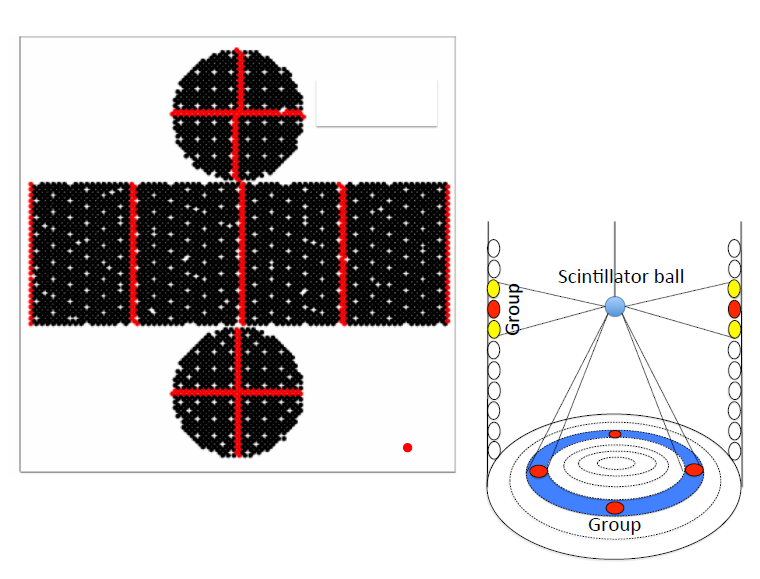
\includegraphics[width=\textwidth]{Figures/hvcalib.png}
\caption{Location of 420 reference PMTs used for HV setting calibration. The red lines in show the placement of these PMTs with repsect to the others (left). The grouping of these PMTs due to their geometry in relation to the light source is also shown (right) }
    \label{fig:hvcalib}
\end{figure}




\subsubsection{Relative gain calibration}

Understanding the timing information from the hit photomultiplier tubes depends on how well the charge from the hit PMT is calculated. To conceive charge calibration, a quantity called photomultiplier tube ''gain" must be calculated. ''Gain" is the conversion factor from the number of photoelectrons produced by the hit PMT and charge, and calibration of this quantity is what interpretation of very high energy events (TeV scale) rely on. Quantum efficiency is another quantity used for the calibration of low energy physics events (such as detection of solar neutrinos), due to them consisting of single photoelectron (single-pe) hits: it is the ratio of the number of the number of photoelectrons emitted by the cathode to the number of photons that are incident on the photomultiplier tube window. Quantum efficiency is particularly useful for low energy events because the number of photons arriving at the photomultiplier tube window is small. Super-Kamiokande calibration converts this measure of quantum efficiency into ''QE" by multiplying the quantum efficiency by the collection efficiency of the photoelectrons onto the first dynode inside the PMT \ref{abeCalibrationSuperKamiokandeDetector2014}. Knowing the gain and QE of each PMT in the detector is important in order to accurately measure the output charge from each individual PMT, which is done by first calculating the relative gain gain difference among all PMTs and then work out the average gain difference over all PMTs in the detector. After this, the variation away from this average gain value can be calculated for each seperate inner detector photomultiplier tube, and the gain value for each can be extracted. 

The relative gain difference is calculated by two measurements using a light source to produce constant-intensity flashes. The first measurement involves using the light source to produce high-intensity flashes so that all photomultiplier tubes in the detctor gets a certain number of photons, and the second measurement has the light source produce low-intensity flashes so that only a few PMTs are hit. teh first measurement provides an average charge value ($Q_{o b s}(i)$) for each inner detector PMT, while the second measurement gives single photoelectron hits, providing a number of times ($N_{o b s}(i)$) that a single PMT gives a charge which is greater than the PMT threshold value. Equation \ref{eq:gaineq} shows how these two values are calculated from the the high and low intensity flash values ($I$), the acceptance of the PMT(i) ($a(i)$), the QE value of the PMT ($\varepsilon_{q e}$) and the PMT gain $G$. 

\begin{align}
Q_{o b s}(i) \quad \propto \quad I_{high} \times a(i) \times \varepsilon_{q e}(i) \times G(i) \\
N_{o b s}(i) \quad \propto \quad I_{low} \times a(i) \times \varepsilon_{q e}(i)
\end{align}
\label{eq:gaineq}

Therefore, by simply dividing these two values of $Q_{o b s}(i)$ and ($N_{o b s}(i)$) the average gain over all PMTs can be calculated.  Figure \ref{fig:relativegain} shows the spread of the relative gain over all the PMTs. 

\begin{figure}
    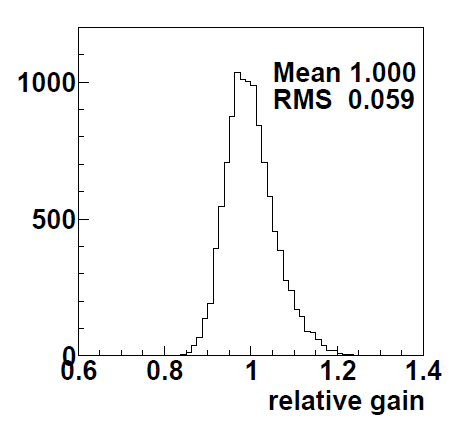
\includegraphics[width=\textwidth]{Figures/relativegain.png}
\caption{Relative gain of PMTs in Super-Kamiokande}
    \label{fig:relativegain}
\end{figure}

\subsubsection{Absolute gain calibration}

In order to calculate absolute gain, the single photoelectron distrubution needs to be measured, this is because absolute gain relates to the observed charge in the photomultplier tube with the number of photoelectrons produced. A nickel source (which includes a Californium-252 which decays to provides a source of neutrons) emits gamma rays in an isotropic distribution after neutron capture. This nickel source is placed in the centre of the inner detector and the gamma rays produced are detetced by all the inner detector PMTs. On average the observed number of photoelectrons is 0.004 per event per PMT, meaning that single p.e. hits are observed for more than 99\% of the hits. The observed charge distribution of all the hits from this nickel source is used to give the average charge, which is used as a conversion factor from a charge measurement in picoColoumbs and single photo-electrons. The factor is 2.658pC per photoelectron (calculated at the beginning of SK-IV) which is then used to extract the single-p.e. distribution, shown in Figure \ref{fig:singlepe}.

\begin{figure}
    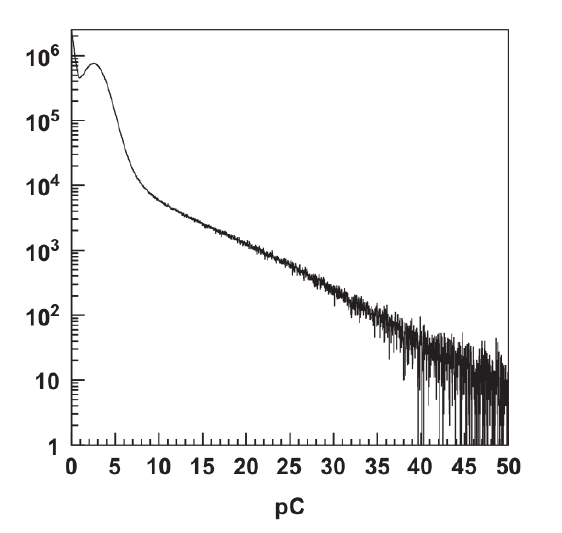
\includegraphics[width=\textwidth]{Figures/singlepe.png}
\caption{Single p.e distribution of charge in pC }
    \label{fig:singlepe}
\end{figure}



\subsubsection{Relative quantum efficiency measurement}

To measure the relative quantum efficiency, the gamma rays from neutron capture on the nickel source are simulated. Inside this simulation, a common value of QE is used for all the ID PMTs to predict the number of hits for each PMT. Comparing this number of hits to the actual data obtained for each individual PMT by calculating the ratio between them provides us with a value for relative QE for each inner detetor PMT which is then used inside the simulation. 

\subsubsection{Timing information calibration}
Calibrating the hit timing information of the photomultiplier tubes is essential due to its importance in accurately being able to reconstruct events. Event reconstruction makes use of determining exactly where interaction vertices are and the direction in which particles travel, and to do this the time response needs to be very carefully calibrated. Differences in how quickly the electronics can process the signal, the length of the cables that carry the signal and the differences in the transit time of the PMTs (the time delay between when the PMT recives a light pulse and the time at which an output pulse appears). The response time of the PMT also relates to the amount of charge observed: in order for a hit to be registered, the PMT signal must pass the discriminator value of the hit threshold, and the time in which this happens is dependent on height of the pulse, which is correlated with observed charge. All thsese factors need to be considered when calibrating hit timing information.
\newline
To aid the timing calibration, a diffuser ball is placed near the centre of the inner detector, into which a nitrogen laser injects pulsed laser light. By varying the intensity of this light, the laser light can be outputted in flashes, and the timing of the laser pulses is monitored using a 2-inch monitor PMT. The schematic of this timing calibration system is shown in Figure \ref{fig:timecalibsystem}.

\begin{figure}
    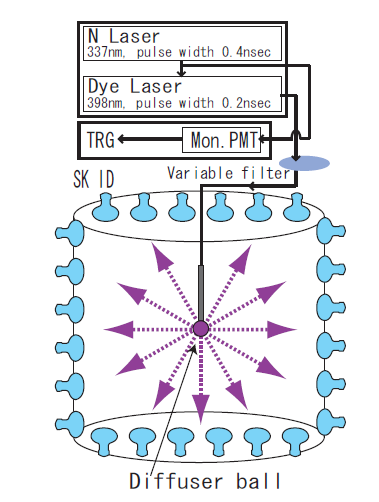
\includegraphics[width=\textwidth]{Figures/timecalibsystem.png}
\caption{Schematic of timing calibration system, with SK ID PMTs in blue and the diffuser ball in purple. The dye laser shifts the wavelength of the laser light to 398 nm to maximise the quantum efficiency of the PMTs and light absorption.}
    \label{fig:singlepe}
\end{figure}


The value of these laser pulse timings, and the time-of-flight value from the diffuser ball are subtracted from the PMT hit time. Using the observed charge values and these adjusted hit times, "TQ" (time and charge) distributions can be plotted for each inner detetector PMT. An example TQ distribution is shown for an inner detector PMT (cable number 00010) in Figure \ref{fig:TQdist}, where the vertical axis shows is the TOF corrected and laser pulse time corrected PMT hit time, the horizontal axis shows the observed charge of each hit. Figure taken from \ref{abeCalibrationSuperKamiokandeDetector2014}. 

\begin{figure}
    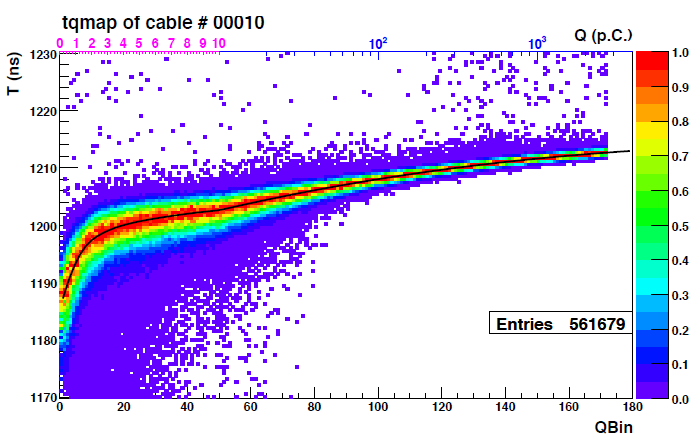
\includegraphics[width=\textwidth]{Figures/TQdist.png}
\caption{Example TQ distribution for an inner detetector PMT}
    \label{fig:TQdist}
\end{figure}


The timing resolution of the PMTs (also known as the transit time spread) is also something that must be calibrated. In photomultiplier tubes, when identical pulses strike the same part of the cathode, there will be fluctuations in the arrival time of the pulse. The timing resolution for a PMT is defined as the full width half maximum of the probability distributions of the fluctuation. This value is proportional to $1/sqrt(n_{k})$ where $n_{k}$ is the number of photoelectrons per pulse. This is calculated by using the same timing and charge data used to produce the TQ distributions. By correcting all the ID PMT hits by their TQ distributions, these residual timing distributions have an asymmetric Gaussian function fitted to them, from which two values of sigma are extracted: $\sigma_{t}$ and $\sigma_{t'}$. These are the values for the timing resolution for before and after the peak time of this distribution. Equation \ref{eq:sigmat} shows how the asymmetric Gaussian is defined. 

***************************************************
ask neil whether this is different to calculating the FWHM of the probability distribution of the fluctuations (definition from the Photonis PMT manual)

*****************************************************

\begin{equation}
    $f\left(t ; t>T_{\text {peak }}\right) \equiv A_{1} \cdot \exp \left(-\left(t-T_{\text {peak }}\right)^{2} / \sigma_{t}^{2}\right)+B_{1}$
    $f\left(t ; t \leq T_{\text {peak }}\right) \equiv A_{2} \cdot \exp \left(-\left(t-T_{\text {peak }}\right)^{2} / \sigma_{t}^{\prime 2}\right)+B_{2}$
    \label{eq:sigmat}
\end{equation}

Figure \ref{fig:resolutiont} shows timing resolution  plotted as a function of charge for both before and after the peak time of the residual time distribution (red and blue points respectively) for SK-IV TQ calibration data. 

\begin{figure}
    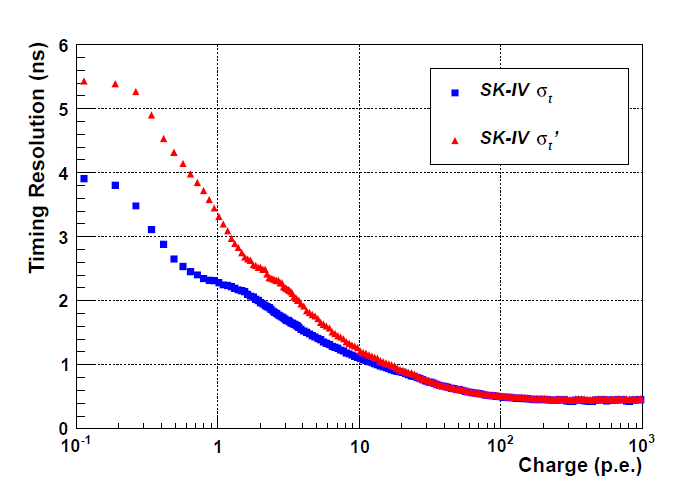
\includegraphics[width=\textwidth]{Figures/resolutiont.png}
\caption{Timing resolution as a function of charge for SK-IV}
    \label{fig:resolutiontt}
\end{figure}

******************************************************
ask neil if there's an updated one for SKV or SKVI or whatever we're in now idk
******************************************************


  \chapter{The UK Light Injection System}
\epigraph{``Photon torpedo: isn't that the universal greeting when communications are down?''\newline
``I think it's the universal greeting when you don't like someone.''}{William T. Riker and Geordi La Forge \newline Star Trek: Insurrection (1998)}
\label{chp:ukli}

The UK calibration group's efforts have been focussed on improving the data analysis method and improving the accuracy of the water coefficient measurements. To aid this effort a new UK developed Light Injection (UKLI) system was installed into Super-Kamiokande during the refurbishment that ocurred in the summer of 2018. This system has its own set of optics with multiple beam spot diameters and will be described in detail in this Chapter. 

\section{The UK Light Injection System Electronics and Optics}

The electronics setup architecture for the UK Light Injection System is made of sixteen light emitting diode boards, where the light being pulsed by the LEDs has a wavelength of 435 nm and there is 1 LED per injector. Each LED is coupled to three optical fibres: one channel connected to a monitor PMT, one connected to an optical fibre that sends light into the Super-Kamiokande detector, and one is a spare.
\newline

Unlike the Korean laser system mentioned in Chapter 4 which injects light into the detector using an optical fibre which has an opening angle of 12 degrees, the UK Light Injection system contains three different types of light injection optics, with each having a different opening angle: a bare fibre, a collimator and a diffuser. This range of optics can accomadate a larger variety of calibration measurements, and better suit the multiple applications of the light injection system. 

\subsubsection{The Collimator Optic}

A 2-degree opening half angle is achieved by the collimator optic by using a GRIN (gradient-index) lens \cite{grin_lens} to reduce the opening angle of the light coming from the fibre optic. A schematic of the collimator design can be seen in Figure \ref{fig:collimator_schematic}. 

\begin{figure}
    \centering
    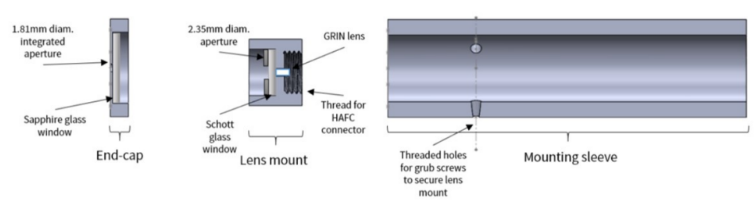
\includegraphics[width=0.8\textwidth]{Figures/collimator_schematic.png}
    \caption{Collimator schematic including the end-cap, lens mount and mounting sleeve structures.}
    \label{fig:collimator_schematic}
\end{figure}


\subsubsection{The Diffuser Optic}

The diffuser optic is a wide angled beam with an opening half-angle of 40 degrees, allowing for more PMT coverage in the detector, therefore enabling measurements of PMT properties, and measurements of light attenuation length in water. Figure \ref{fig:diffuser_photo} shows a photograph of one of the diffusers used, and one of the diffuser ball enclosures. The enclosure is made of high grade stainless steel and using a chemical and water resistant epoxy resin, so all the components were ensured to be watertight. 

\begin{figure}
    \centering
    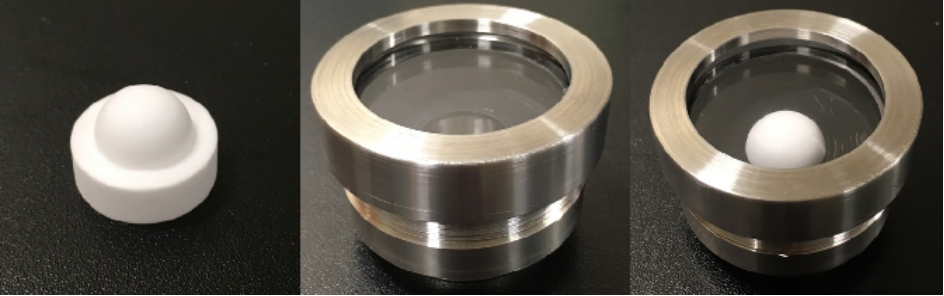
\includegraphics[width=0.7\textwidth]{Figures/diffuser_photo.png}
    \caption{Photograph of the diffuser by itself (left), empty diffuser enclosure (centre) and diffuser inside enclosure (right).}
    \label{fig:diffuser_photo}
\end{figure} 

\subsubsection{Bare Fibre and Optical Plate}

The bare fibre injector are 1 mm step index fibres, are approximately 20 cm in length and are used for validation purposes with the bare fibres in the Korean optical calibration system. These short fibres are screwed into the back end of the optical plate that the collimator and diffuser optics are mounted on, shown in Figure \ref{fig:optical_plate}.

\begin{figure}
    \centering
    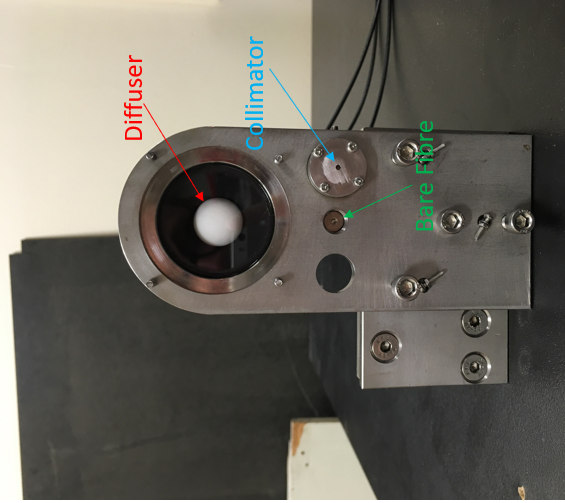
\includegraphics[width=0.7\textwidth, angle =270]{Figures/optical_plate.png}
    \caption{Photograph of the optical plate which houses the different optics.}
    \label{fig:optical_plate}
\end{figure}


\section{Optics test stand measurements}

In order to test the collimator and diffuser optics, measurements of the angular distributions were made using diffuser and collimator test-stands and would measure angular distributions of the light intensity. The setup for the collimator test stand at the University of Warwick is shown in Figure \ref{fig:coll_test_stand} and captures the beam cross section by moving a CMOS camera along the beam width. For the diffuser test-stand the angular distribution of the light output was measured using the setup shown in Figure \ref{fig:diffuser_test_stand}. This test stand setup for the diffuser optics consists of a test diffuser ball placed inside a diffuser enclosure, a rotation stage which allows for the movement of the diffuser between -40 and 40 degrees, and a PMT used for pulse intensity measurement set up 250 mm away from the diffuser. An optical fibre couples the diffuser under test to a laser set to a wavelength of 450 nm. 

\begin{figure}
    \centering
    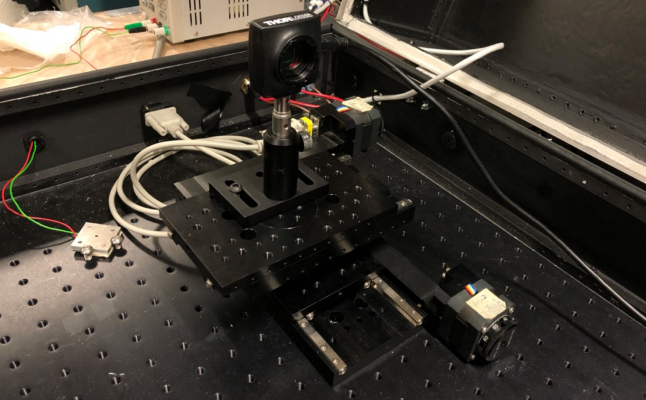
\includegraphics[width=0.7\textwidth]{Figures/coll_test_stand.png}
    \caption{Setup of the collimator test stand provided by the University of Warwick.}
    \label{fig:coll_test_stand}
\end{figure}

Figure \ref{fig:collimator_TF1} shows fits made by ROOT to the light profiles for the collimator. The angular distributions shown give the distribution of the polar angle in degrees of light intensity which are relative to the virtual position from which the light cone originates, averaged over all the orientations of the azimuthal angle. 

\begin{figure}[!htbp]
    \centering
    
    
    
    \subfloat[]{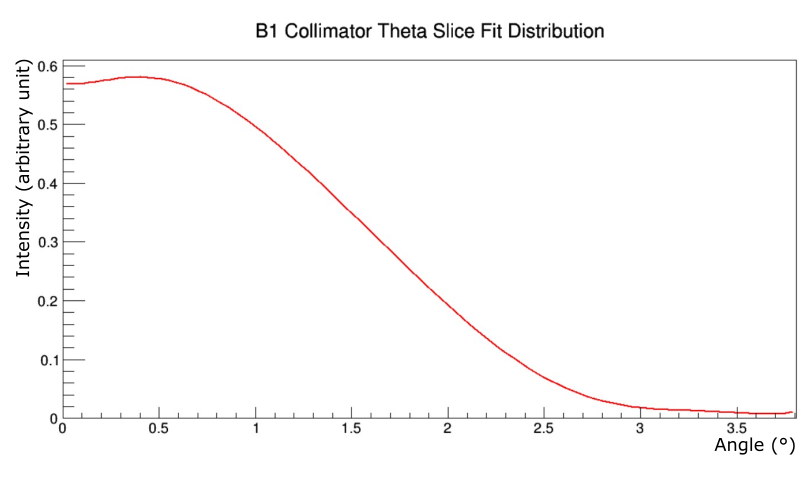
\includegraphics[width=0.49\textwidth]{Figures/B1_collimator_fit.PNG}}\hfill
    \subfloat[]{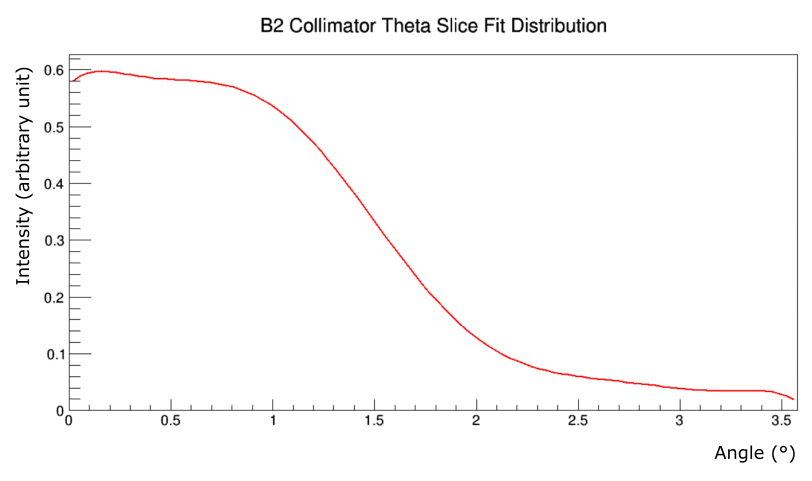
\includegraphics[width=0.49\textwidth]{Figures/B2_collimator_fit.PNG}}\par
    \subfloat[]{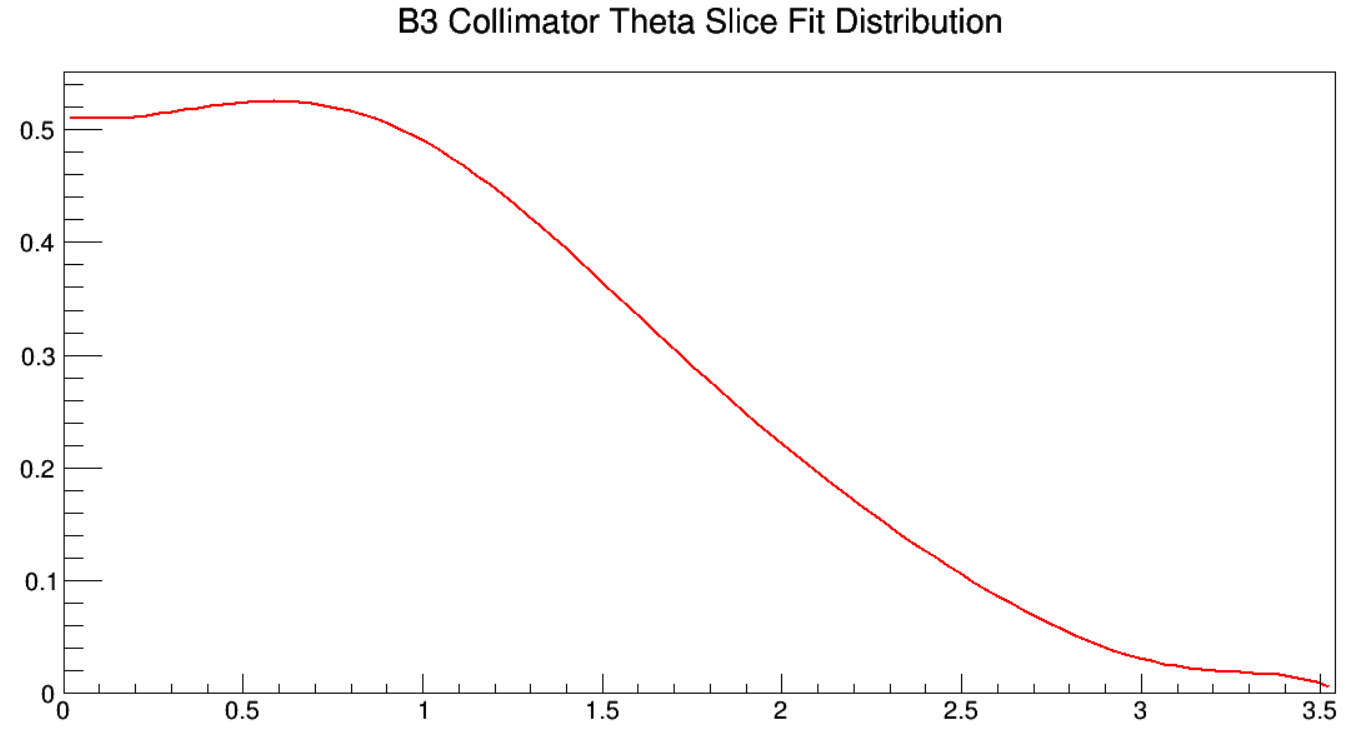
\includegraphics[width=0.49\textwidth]{Figures/B3_collimator_fit.PNG}}\hfill
    \subfloat[]{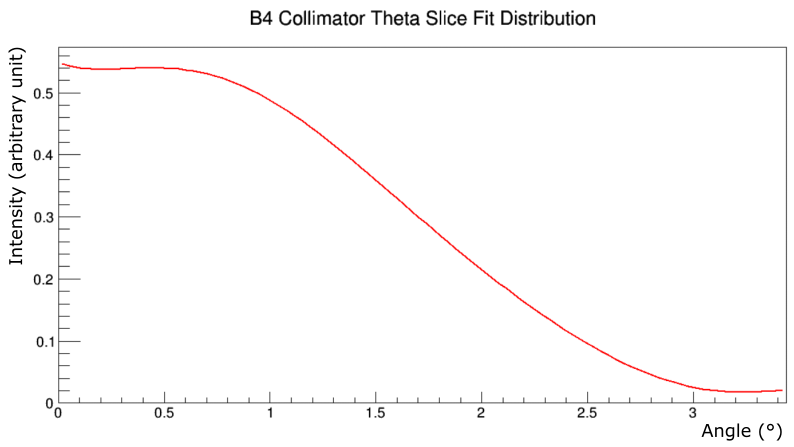
\includegraphics[width=0.49\textwidth]{Figures/B4_collimator_fit.PNG}}\par
    \subfloat[]{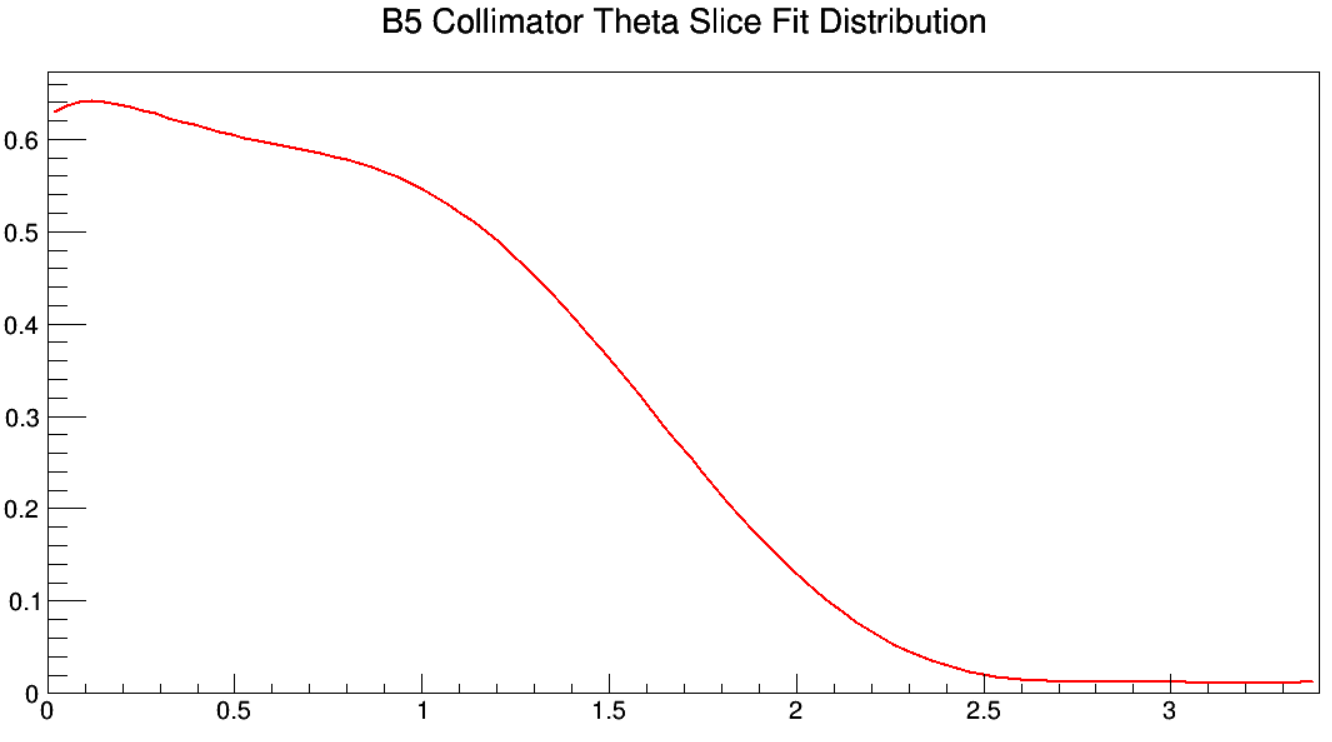
\includegraphics[width=0.49\textwidth]{Figures/B5_collimator_fit.PNG}}

    \caption{Light profiles for the collimator optics provided by the University of Warwick. The profile for each barrel collimator (B1-B5) is shown in (a)-(e) respectively. The light intensity in arbitrary units is shown on the y-axis, while the polar angle of the light is shown on the x-axis.}\label{fig:collimator_TF1}
\end{figure}



\begin{figure}
    \centering
    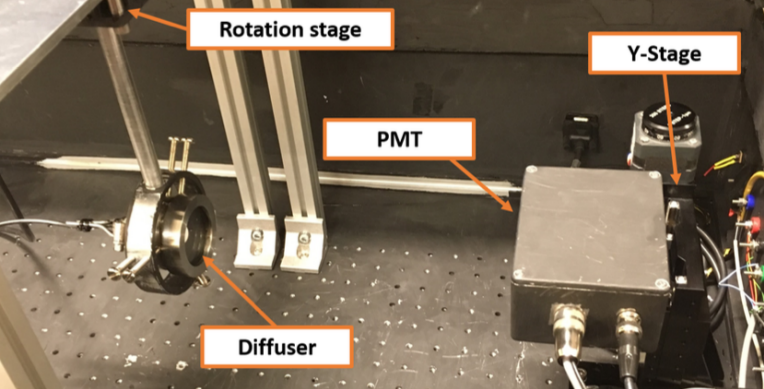
\includegraphics[width=0.7\textwidth]{Figures/diffuser_test_stand.png}
    \caption{Setup of the diffuser test stand provided by the University of Warwick.}
    \label{fig:diffuser_test_stand}
\end{figure}

Figure \ref{fig:diffuser_TF1} shows distributions provided by this test stand data which are preliminary fits made by ROOT to the light profiles for the diffuser. These distributions are not phi-averaged, and instead are scans across the front of the diffuser. The asymmetries in the profile intensities between -40$\degree$ and 0$\degree$ and 0$\degree$ and 40$\degree$ are due to imperfections in the diffuser balls and their enclosures. 

\begin{figure}[!htbp]
    \centering
    
    \caption{Light profiles for the diffuser optics provided by the University of Warwick. The profile for each barrel diffuser (B1-B5) is shown in (a)-(e) respectively. The light intensity in arbitrary units is shown on the y-axis, while the polar angle scan of the light across the diffuser is shown on the x-axis.}\label{fig:diffuser_TF1}
    
    \subfloat[]{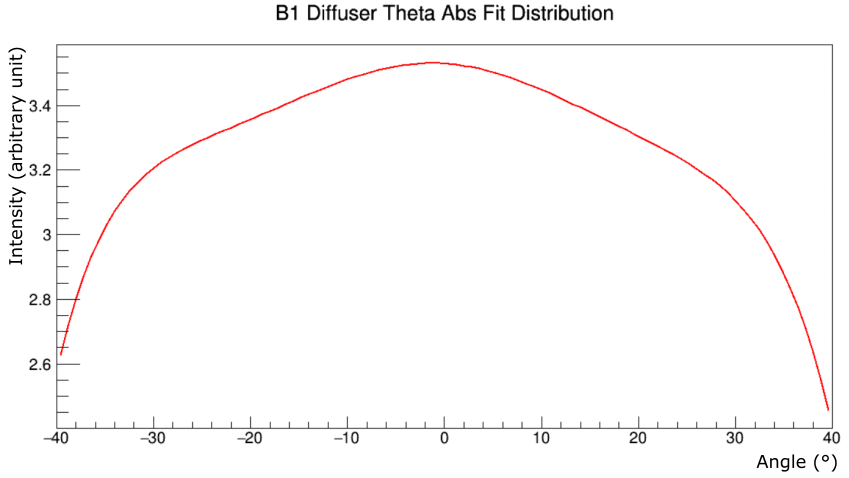
\includegraphics[width=0.49\textwidth]{Figures/B1_diffuser_fit.PNG}}\hfill
    \subfloat[]{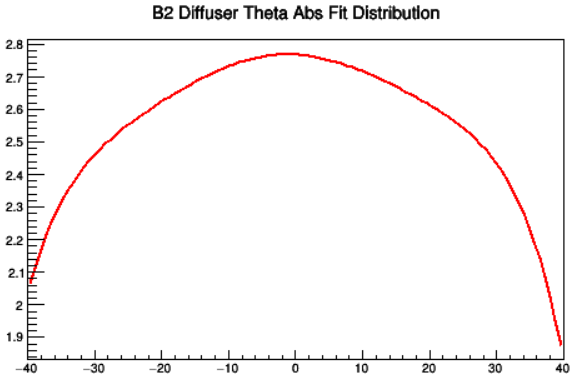
\includegraphics[width=0.49\textwidth]{Figures/B2_diffuser_fit.PNG}}\par
    \subfloat[]{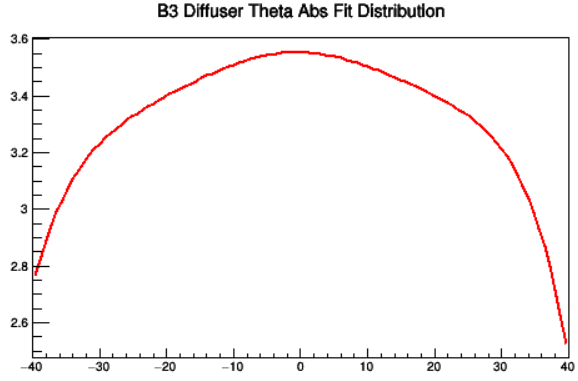
\includegraphics[width=0.49\textwidth]{Figures/B3_diffuser_fit.PNG}}\hfill
    \subfloat[]{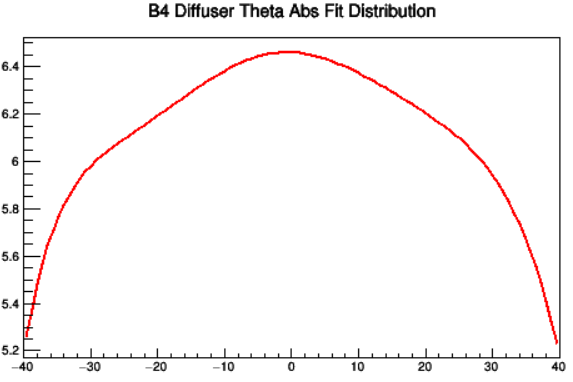
\includegraphics[width=0.49\textwidth]{Figures/B4_diffuser_fit.PNG}}\par
    \subfloat[]{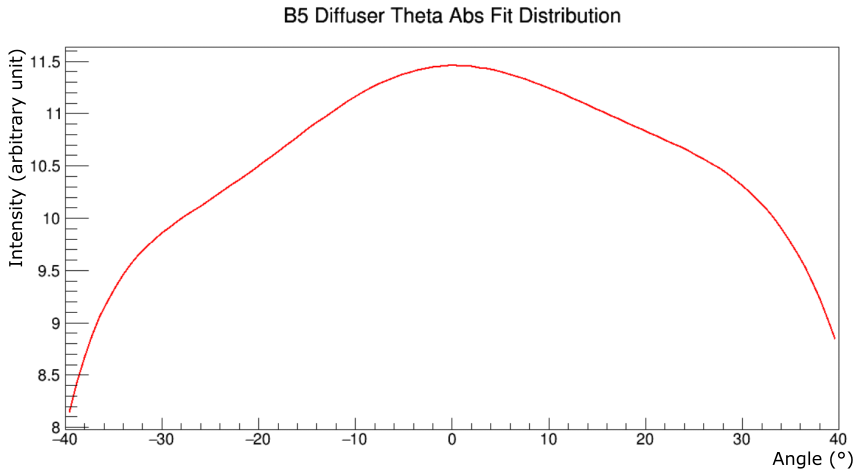
\includegraphics[width=0.49\textwidth]{Figures/B5_diffuser_fit.PNG}}
    
\end{figure}






\section{First commissioning data from UKLI}

In September of 2019 and November of 2019 two sets of test data were taken of the collimator, the diffuser and the bare fibre optic (the B2 bare fibre) and using an event display developed by the University of Warwick, occupancy plots of the test data sets were produced. Figure \ref{fig:occupancy_coll} shows the occupancy plots for the collimator optic from the November 2019 dataset showing the beam spot inside the unrolled volume of the Super-Kamiokande detector. Similarly, Figure \ref{fig:occupancy_diffuser} shows the occupancy plots for the diffuser optic from the November 2019 dataset. The graph in the bottom right hand corner of the occupancy plots show the corrected time-of-flight plots for the PMT hits from the injector. The intensely dark purple hits in Figure \ref{fig:occupancy_diffuser} are ``hot channels'' and have not been accounted for - these should not be mistaken for scattered hits.



\begin{figure}
    \centering
    
    \caption{Occupancy plots for the collimator optics from the UKLI November 2019 test run for each barrel collimator in the unrolled volume of the SK detector. The crosses show the injector positions, and the collimator beam spots are also shown (the PMTs with highest occupancy). The corrected time-of-flight plots for the PMT hits is shown in the bottom right corner.}
    \label{fig:occupancy_coll} 
    \subfloat[B1 collimator]{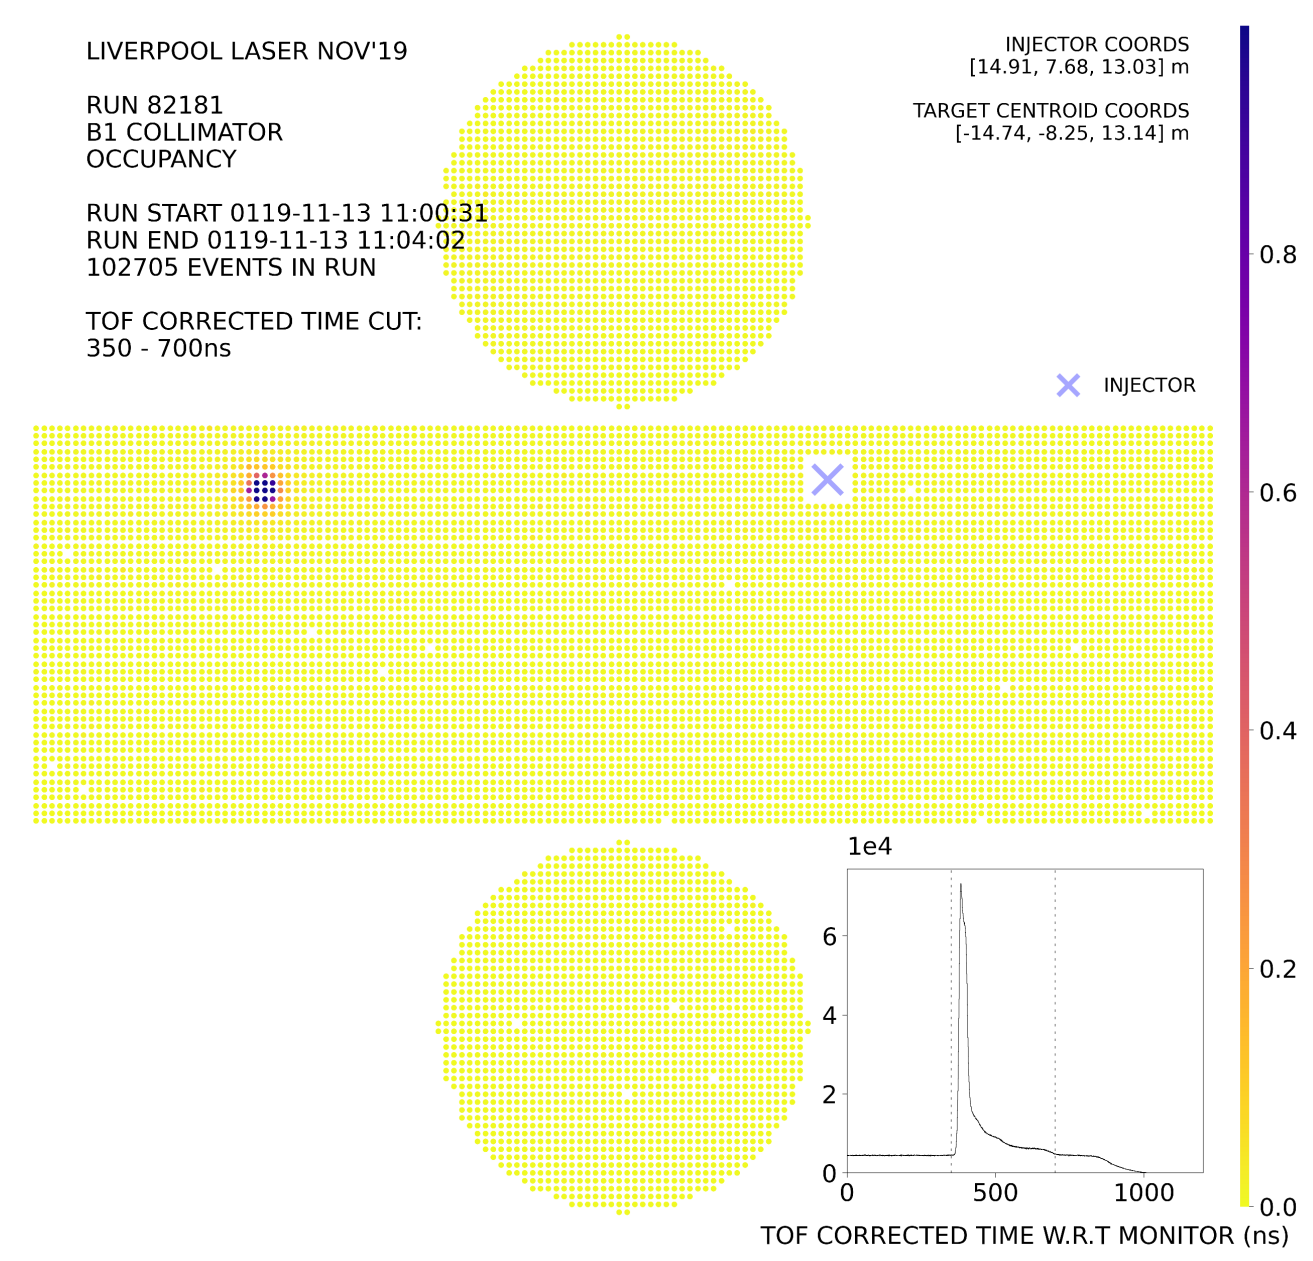
\includegraphics[width=0.49\textwidth]{Figures/B1_occupancy_coll.PNG}} \hfill
    \subfloat[B2 collimator]{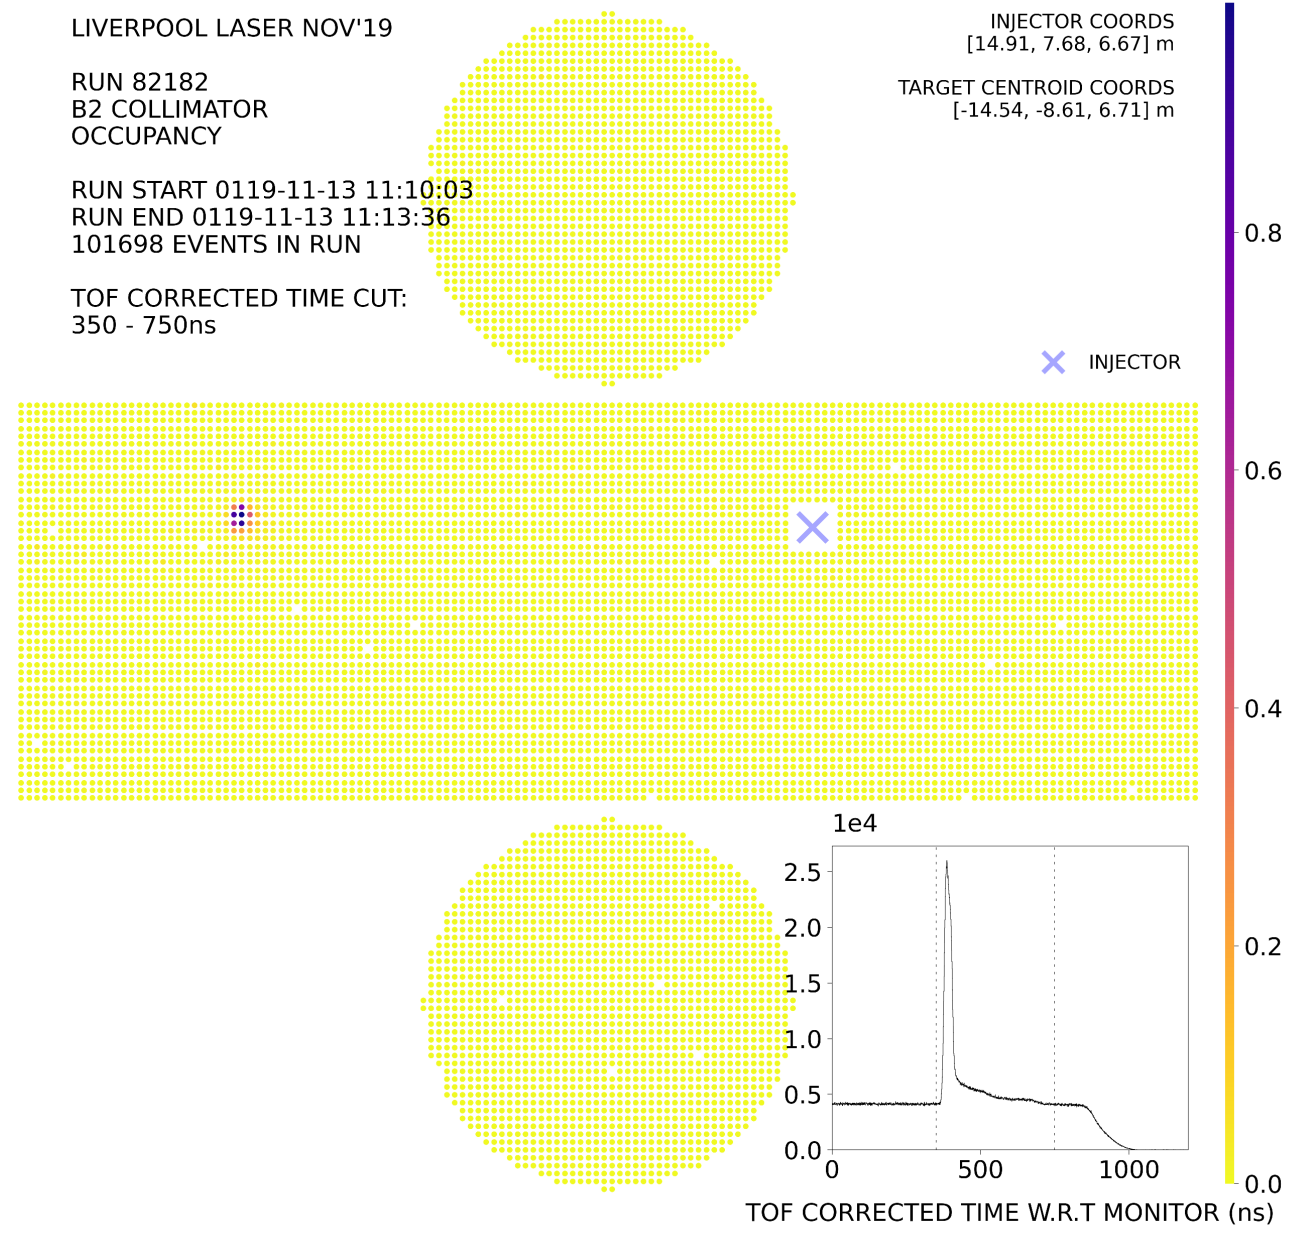
\includegraphics[width=0.49\textwidth]{Figures/B2_occupancy_coll.PNG}} \par
    \subfloat[B3 collimator]{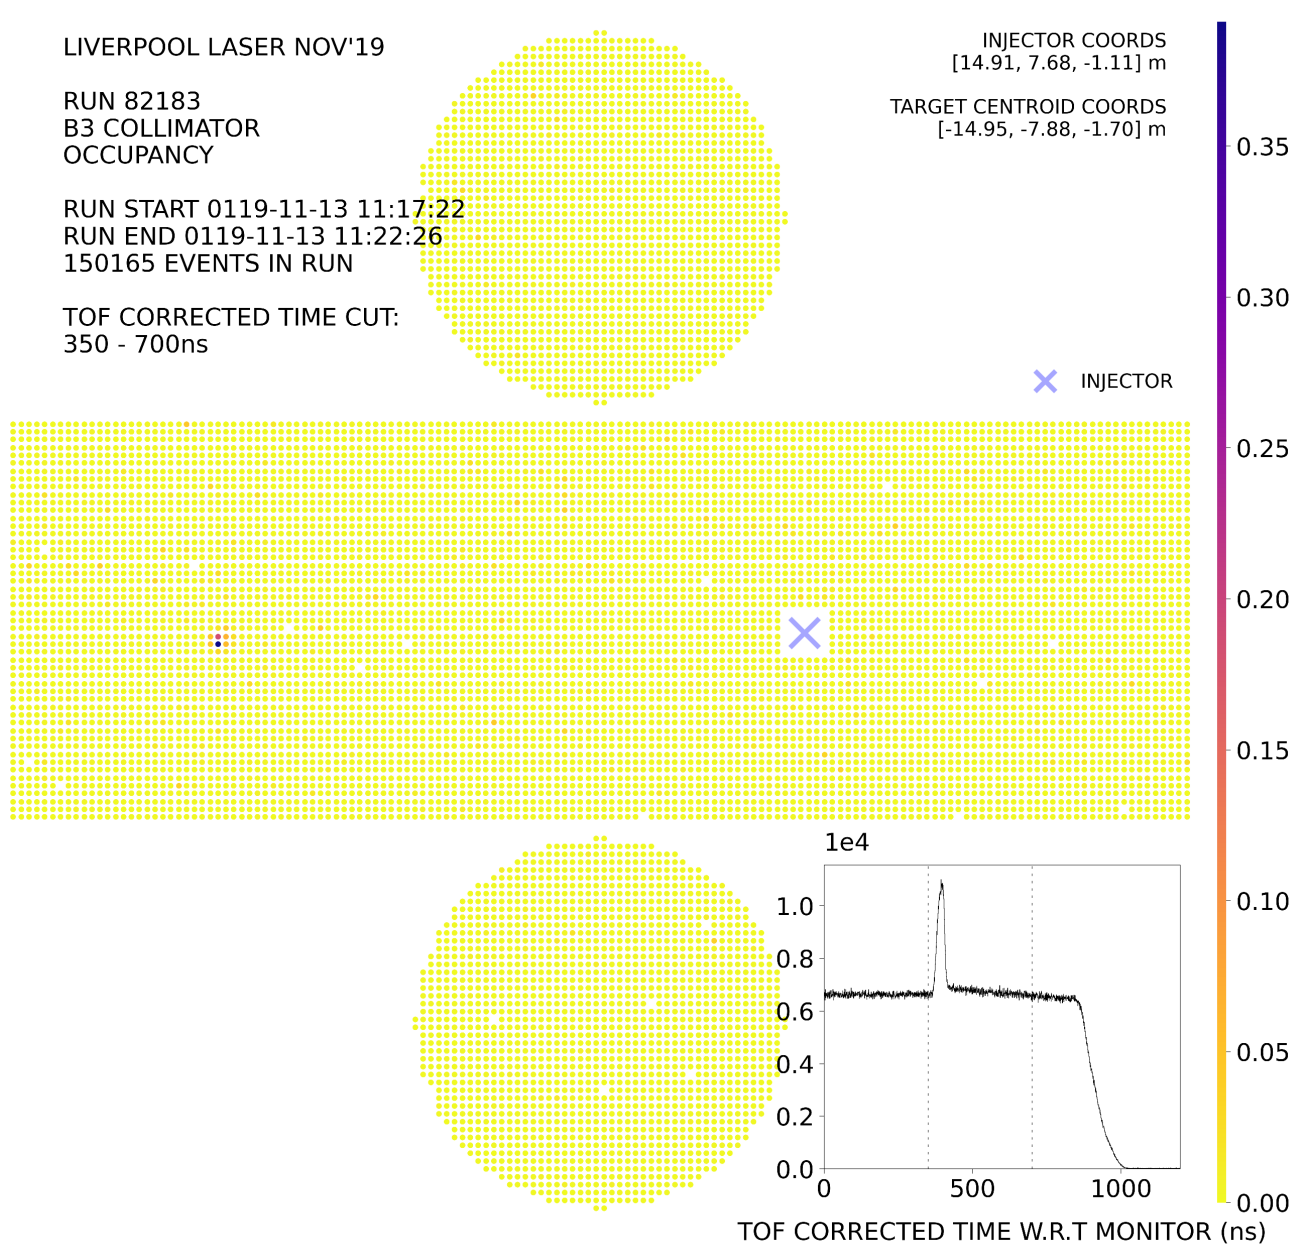
\includegraphics[width=0.49\textwidth]{Figures/B3_occupancy_coll.PNG}} \hfill
    \subfloat[B4 collimator]{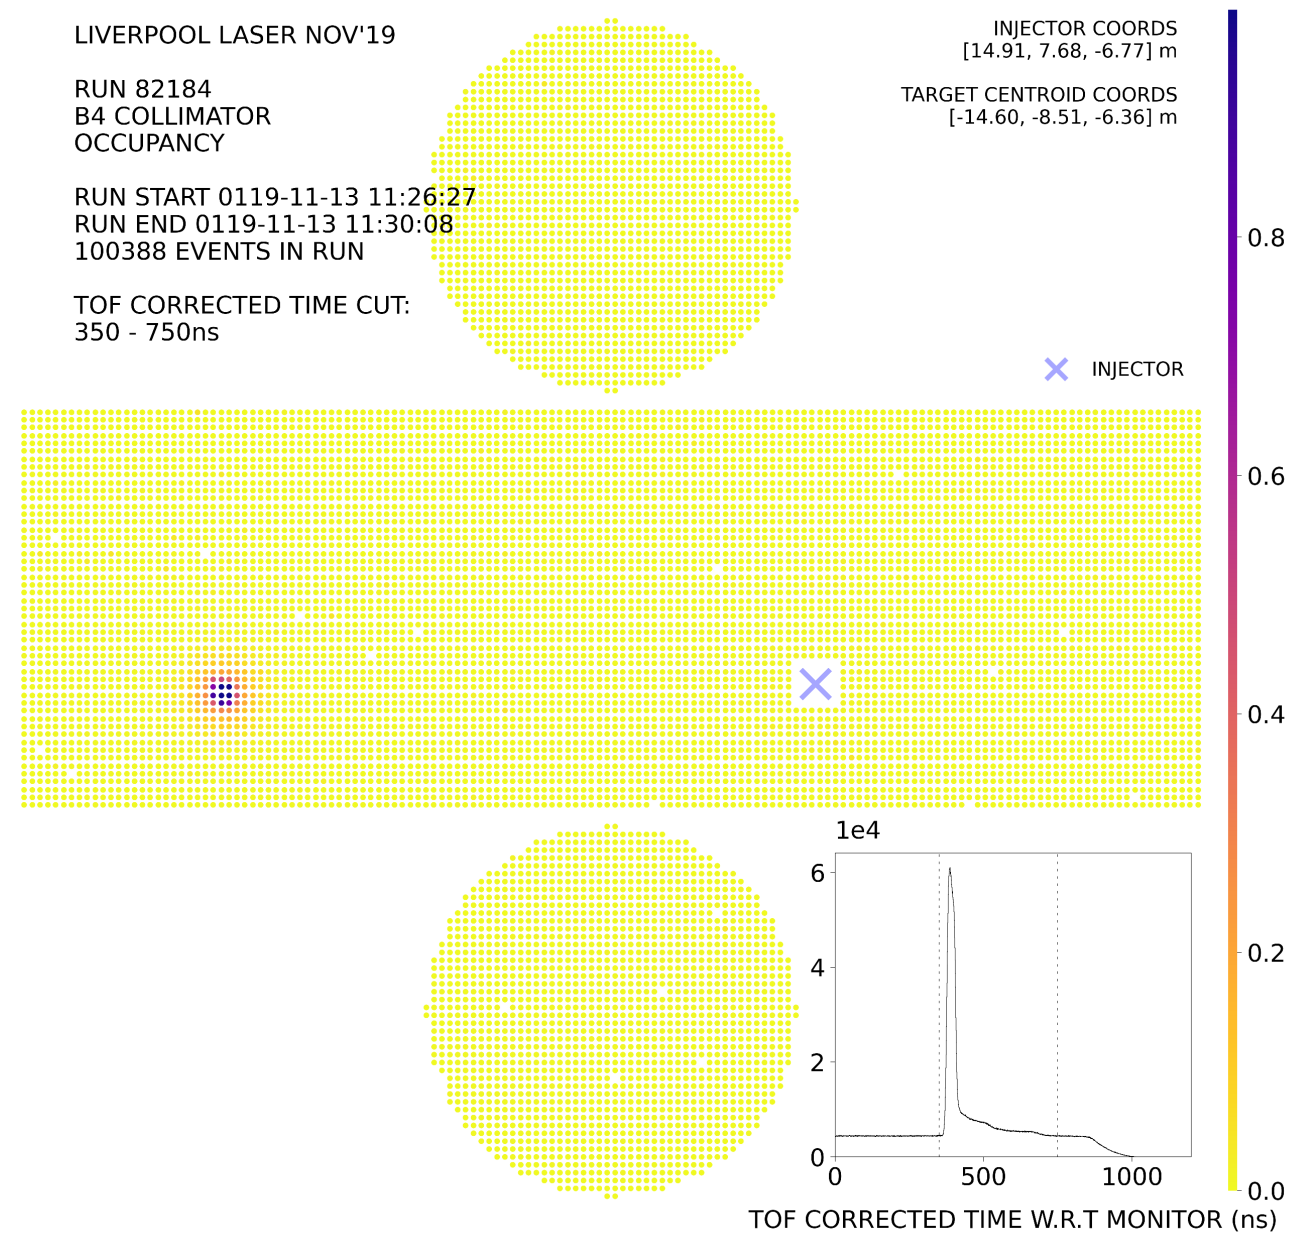
\includegraphics[width=0.49\textwidth]{Figures/B4_occupancy_coll.PNG}} \par
    \subfloat[B5 collimator]{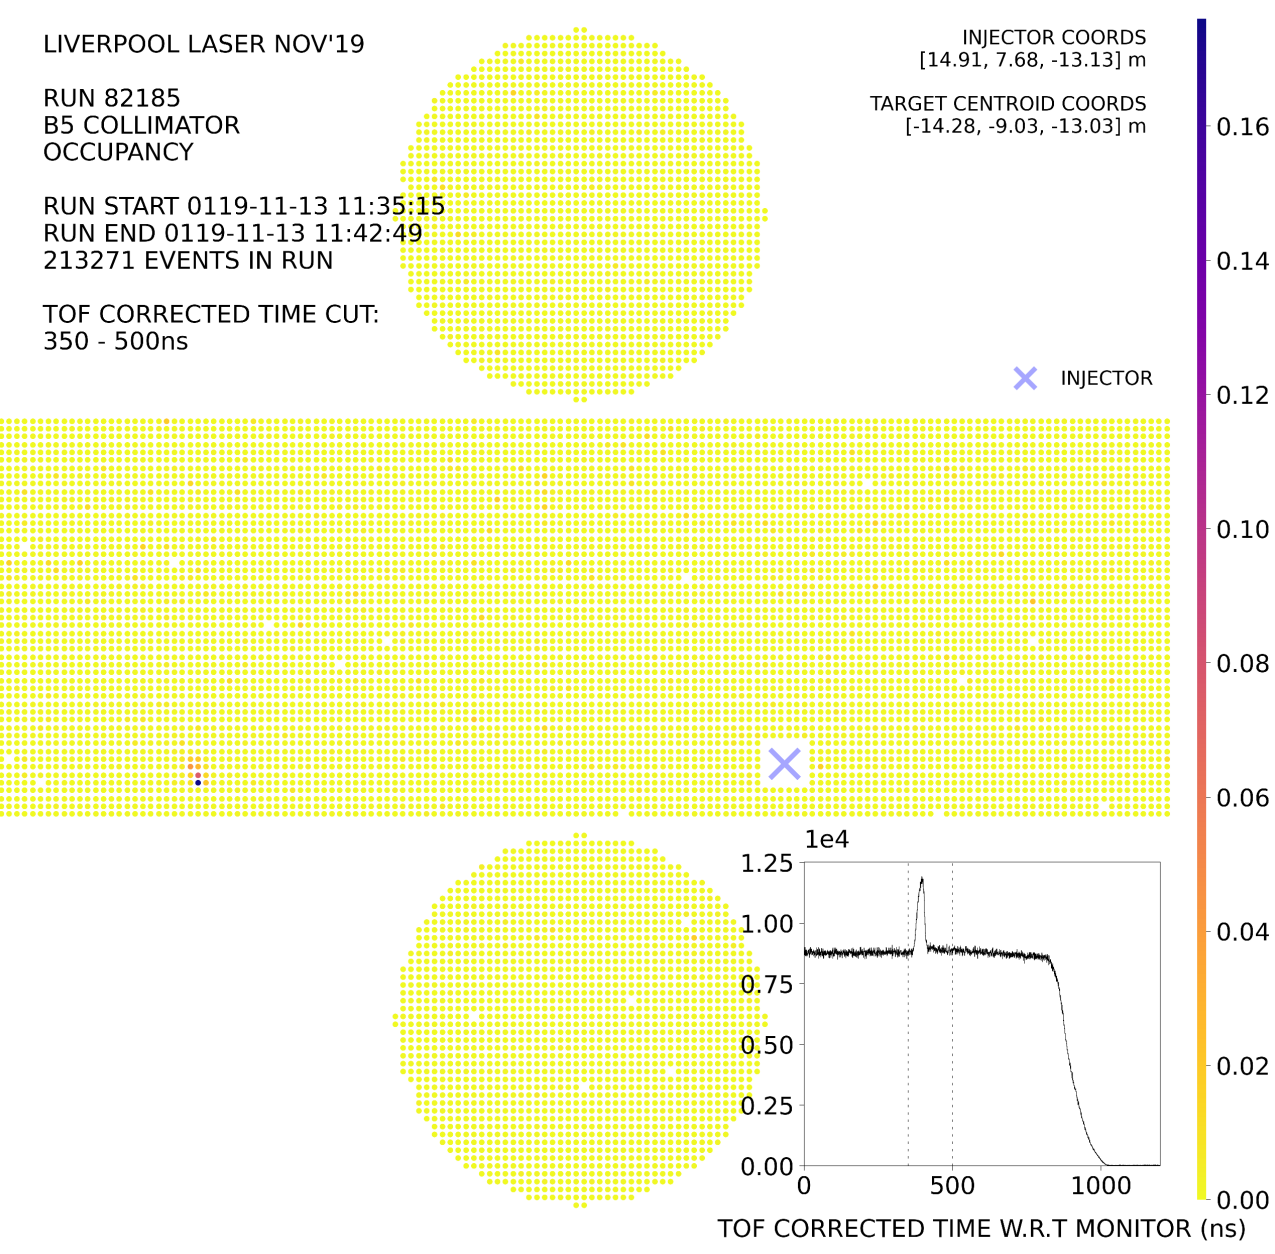
\includegraphics[width=0.49\textwidth]{Figures/B5_occupancy_coll.PNG}}
    \thisfloatpagestyle{empty}
\end{figure}


\begin{figure}
    \centering
    
    \caption{Occupancy plots for the diffuser optics from the UKLI November 2019 test run, where the injector positions are shown by crosses. The corrected time-of-flight plots for the PMT hits is shown in the bottom right corner.} \label{fig:occupancy_diffuser} 
    
    \subfloat[B1 diffuser]{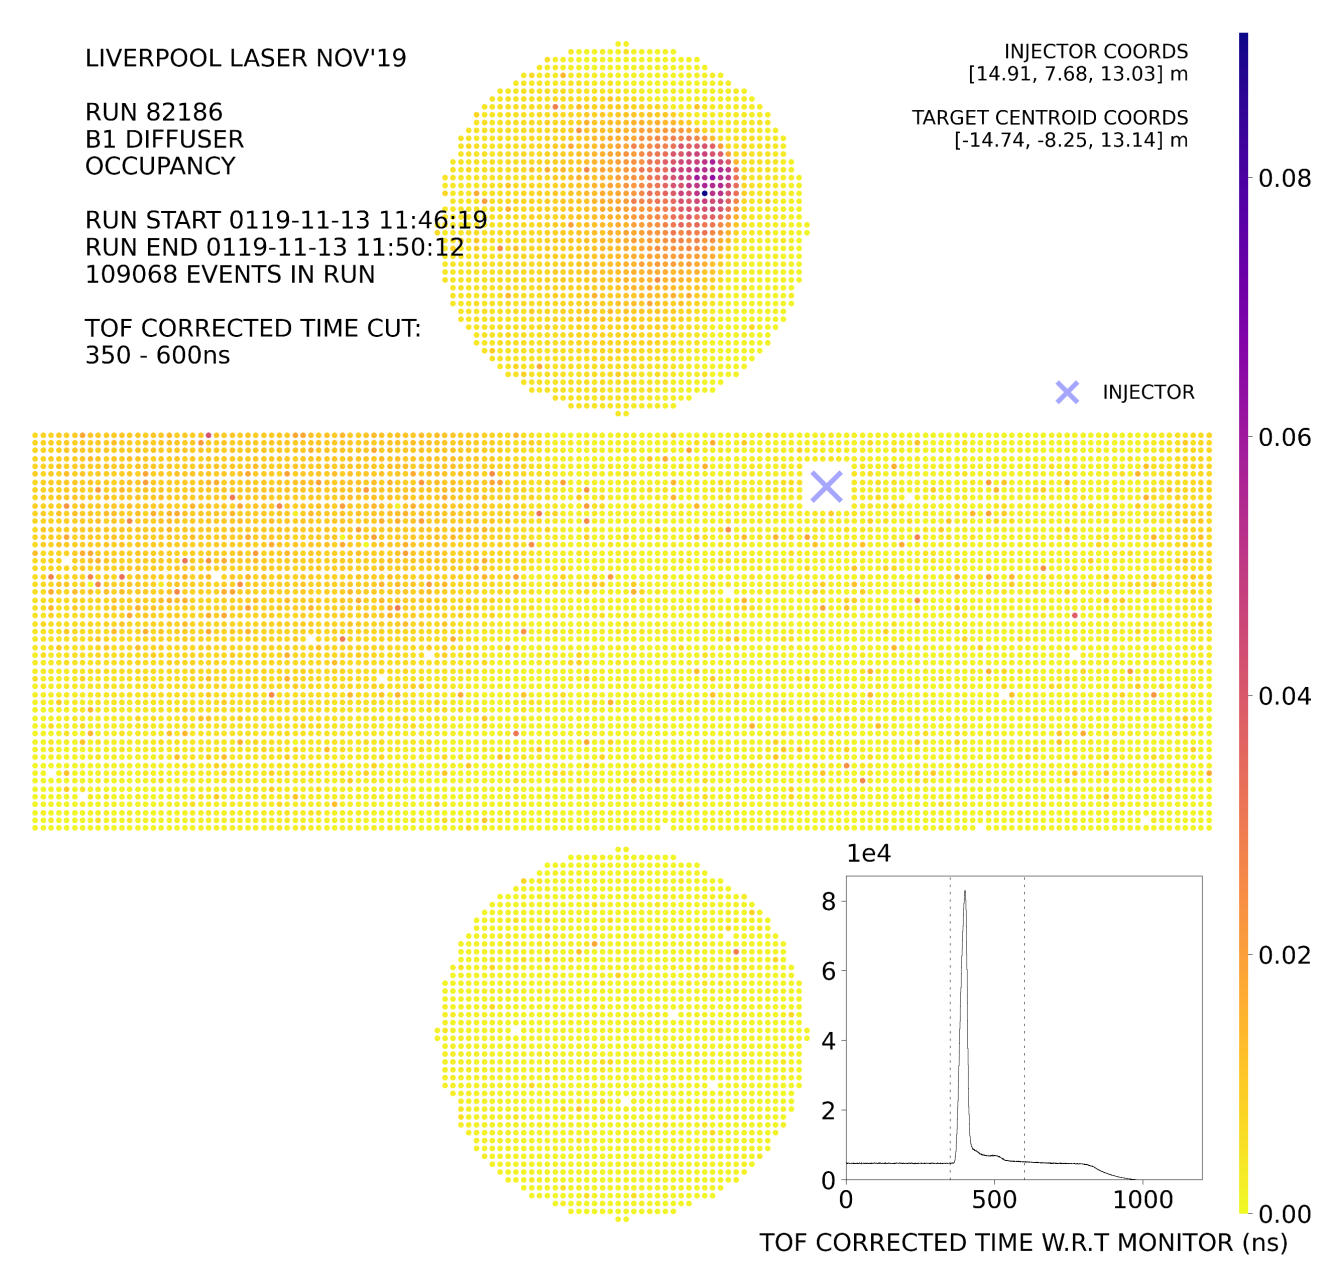
\includegraphics[width=0.49\textwidth]{Figures/B1_occupancy_diff.PNG}} \hfill
    \subfloat[B2 diffuser]{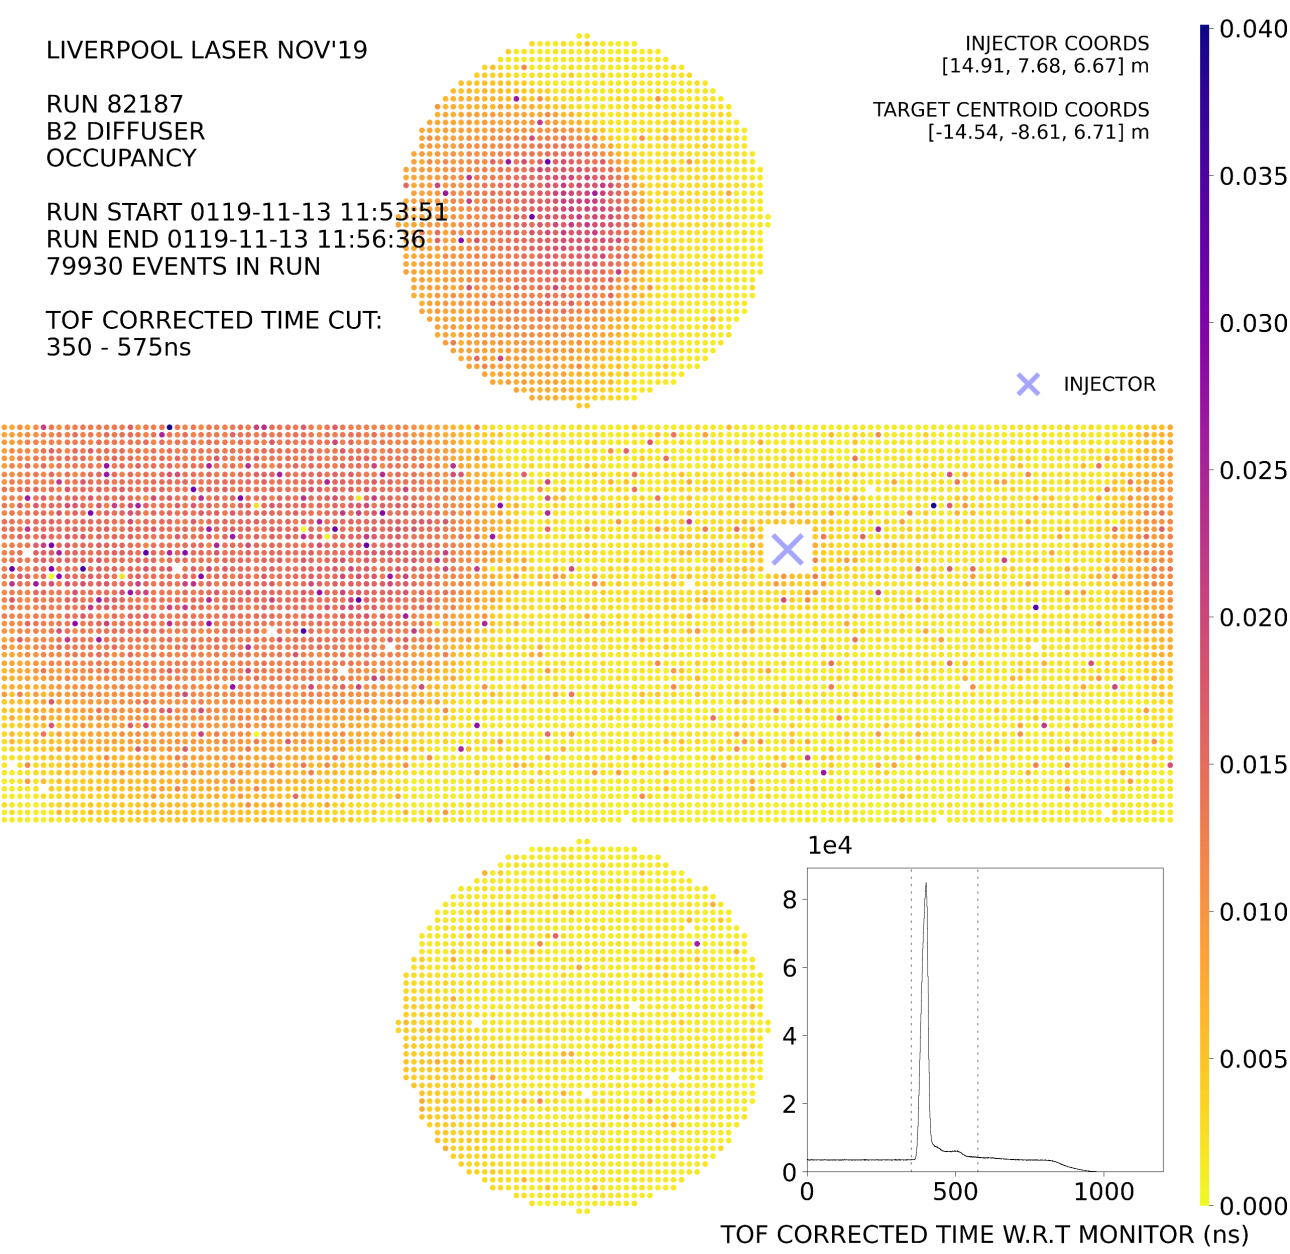
\includegraphics[width=0.49\textwidth]{Figures/B2_occupancy_diff.PNG}} \par
    \subfloat[B3 diffuser]{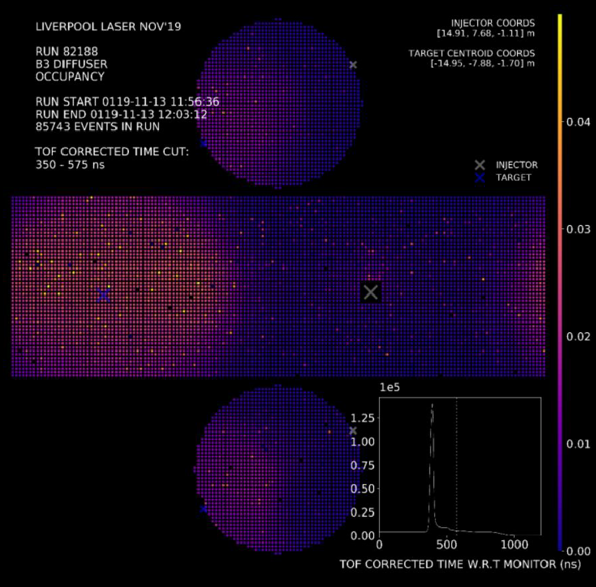
\includegraphics[width=0.49\textwidth]{Figures/B3_occupancy_diff.PNG}} \hfill
    \subfloat[B4 diffuser]{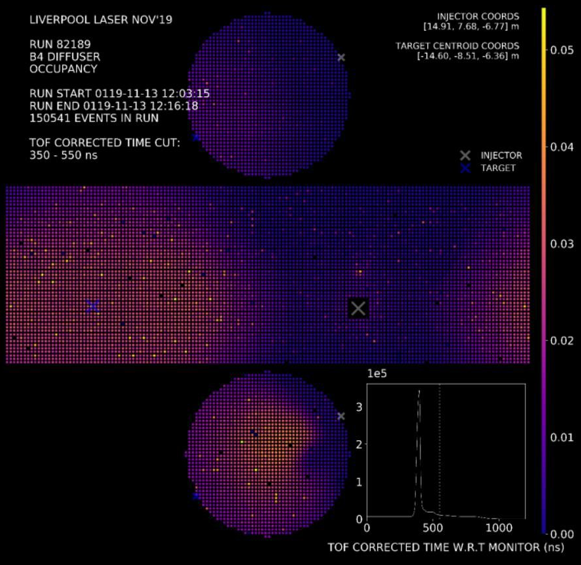
\includegraphics[width=0.49\textwidth]{Figures/B4_occupancy_diff.PNG}} \par
    \subfloat[B5 diffuser]{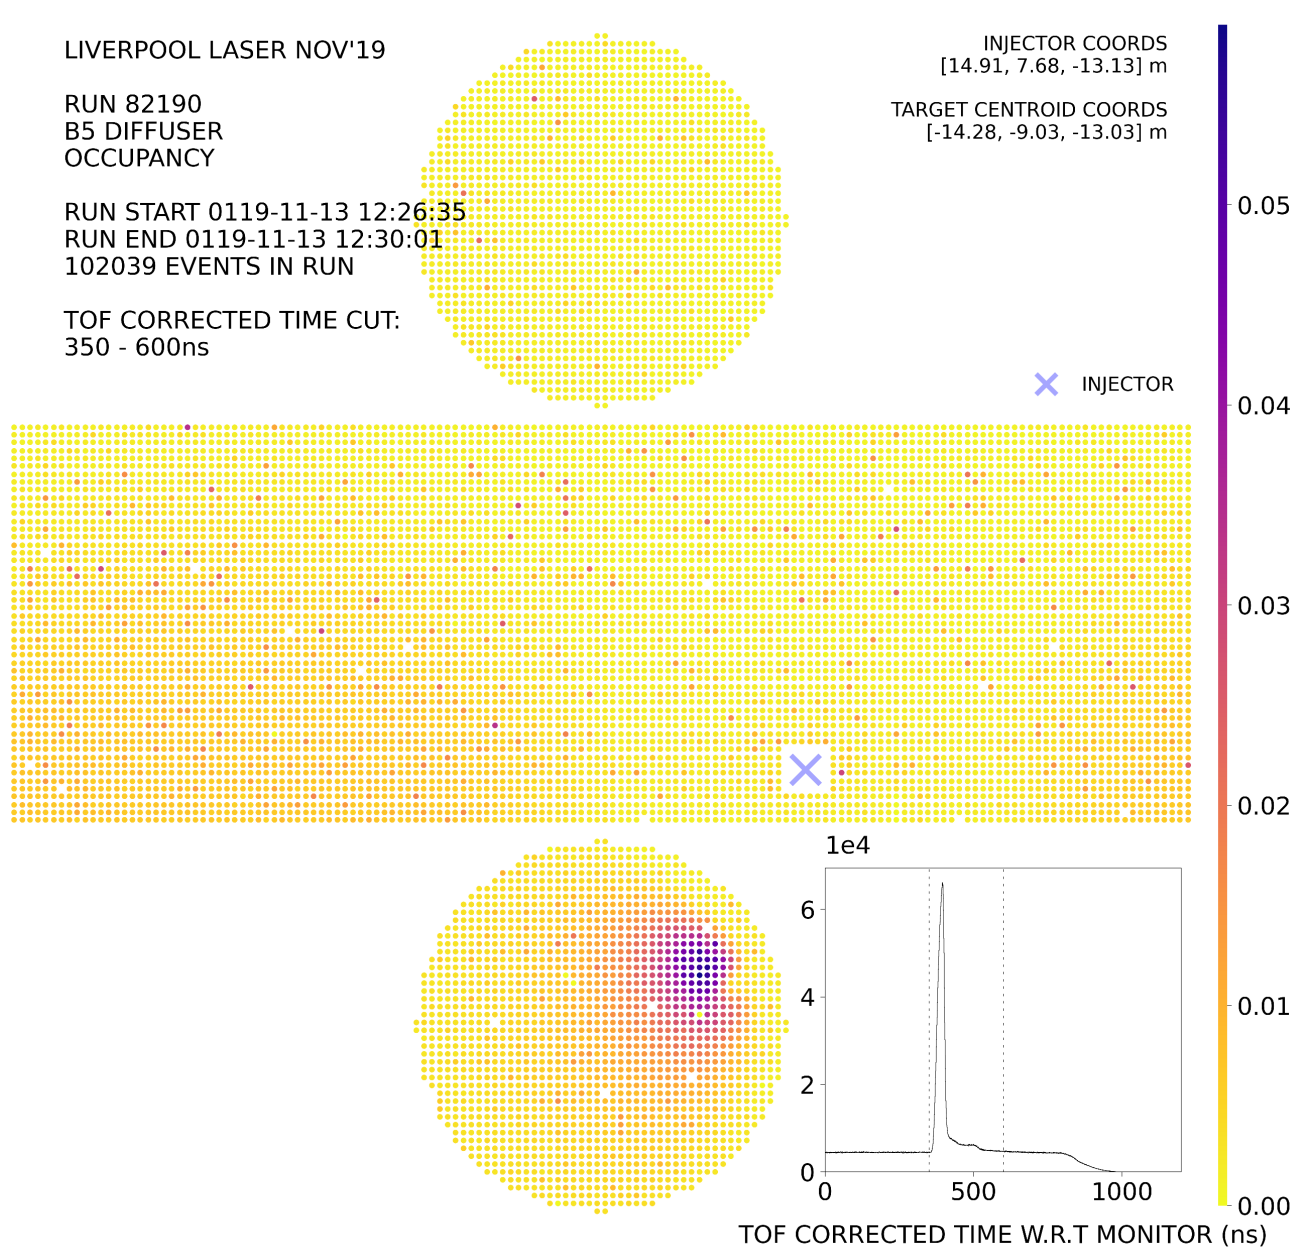
\includegraphics[width=0.49\textwidth]{Figures/B5_occupancy_diff.PNG}}
    
\end{figure}

The UKLI was also added to the ``autocalib'' system used for long term monitoring of the water parameters in Super-Kamiokande by the Korean laser system. In early 2020 the autocalib scheduler was modified to incorporate data taking by the UKLI system which was very useful for gadolinium loading calibration purposes but also in the longer term, it will be useful in the monitoring of daily/weekly water coefficient property measurements, investigation of depth dependence with respect to the water properties and PMT property calibration. Figure \ref{fig:autocalib} shows the schedule for autocalib, and the black dashed lines show the position of the UK barrel collimator and diffusers with respect to the other autocalib data taking streams. The horizontal blue line shows the length of the one autocalib cycle, which is about 4.6 seconds, with each UKLI optic taking about 3310 events per day. 

\begin{figure}
    \centering
    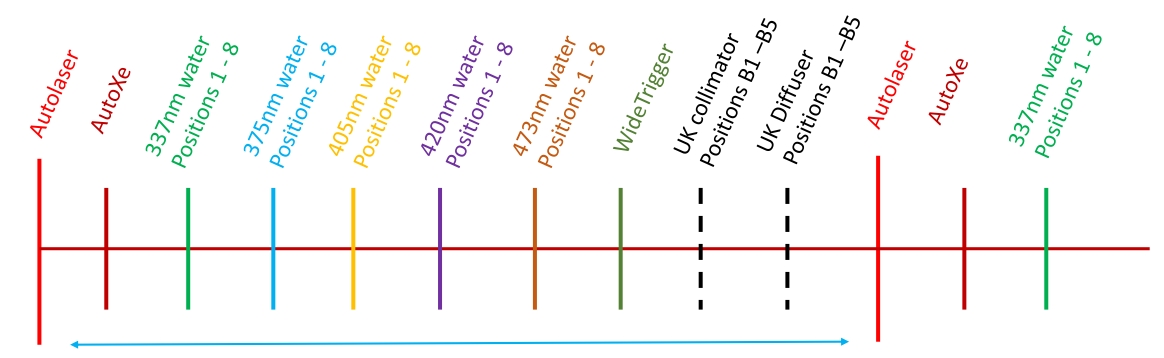
\includegraphics[width=0.8\textwidth]{Figures/autocalib.png}
    \caption{Schematic showing position of the UKLI in autocalib scheduler: the black dashed lines show the UKLI B1-B5 collimator and diffuser optics and the horizontal blue line shows the length of one autocalib cycle.}
    \label{fig:autocalib}
\end{figure}

Figures \ref{fig:B1_coll_auto_July} and \ref{fig:B1_diff_auto_July} show the occupancy plots for autocalib data taken in July 2020, for the B1 collimator and the B1 diffuser respectively. From this point onwards all plots relating to the B2 - B5 injectors for both the collimators and diffusers will be shown in Appendix A. As can be seen in the text in the upper left hand corner, the number of events in the run is a lot less than the 100,000 events or so taken in the test runs, however they are more than sufficient for monitoring purposes.


\begin{figure}
    \centering
    
    \begin{minipage}{0.47\textwidth}
        \centering
        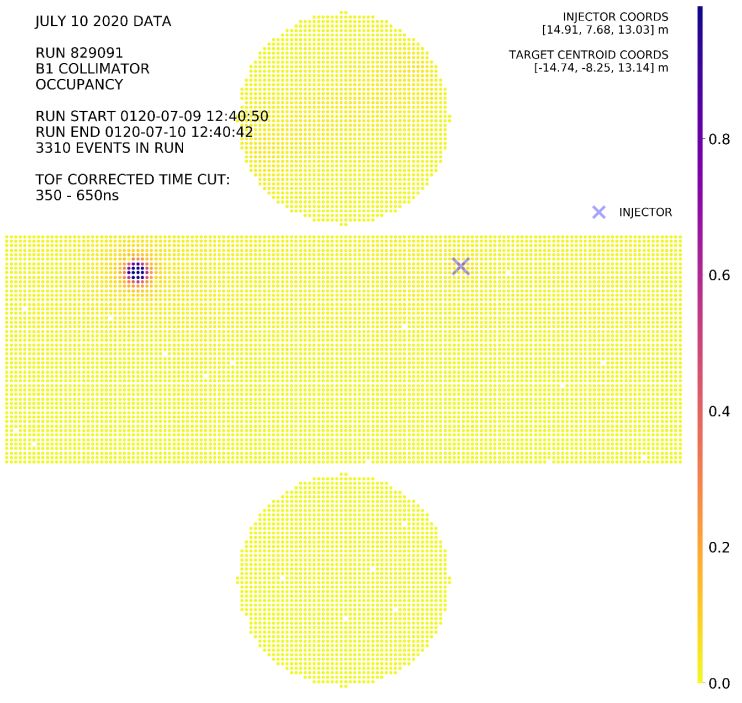
\includegraphics[width=\textwidth]{Figures/B1_occupancy_coll_auto.PNG} % first figure itself
        \caption{Occupancy plot for the B1 collimator optic from the UKLI Autocalib July 2020 run.}
        \label{fig:B1_coll_auto_July}
    \end{minipage}\hfill
    \begin{minipage}{0.47\textwidth}
        \centering
        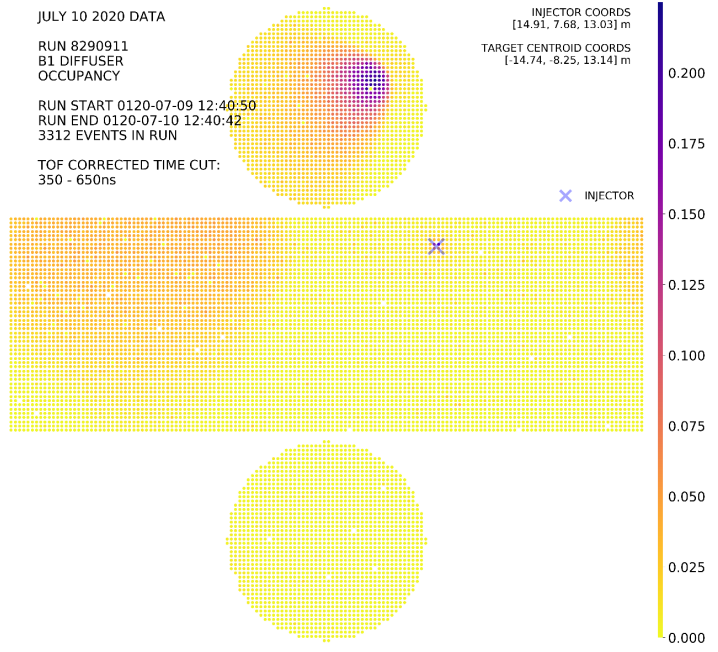
\includegraphics[width=\textwidth]{Figures/B1_occupancy_diff_auto.PNG} % second figure itself
        \caption{Occupancy plot for the B1 diffuser optic from the UKLI Autocalib July 2020 run.}
        \label{fig:B1_diff_auto_July}
    \end{minipage}
\end{figure}


\section{Implementation of UKLI in SK Simulation}
In order to simulate the data taken with the UKLI, SKDETSIM \cite{harada2019development}, the Super Kamiokande Detector Simulator was used. SKDETSIM uses GEANT3 (GEometry ANd Tracking 3 \cite{geant3_cite}) to simulate what the particles in each event would do inside the detector, and tracks the particle's trajectories and energy loss. Simulating the light injection from the UKLI system in SKDETSIM was done in a similar way to the Korean method of producing Monte Carlo: the same versions of the calibration scripts were used, however, small modifications were made to them and to the version of SKDETSIM used to simulate the input photons from the system in the detector. The calibration software allows for the number of events and the number of injected photons to be set, in order to generate many Monte Carlo files with varying absorption, Rayleigh and Mie scattering parameters. 
\newline
Along with making sure the position of the injectors was set to that of the UKLI injectors (shown in Table \ref{table:UKLI_loc}), the opening angle of the injectors determined by the simulation had to be set to accomodate the fact that the injectors for the UKLI system now consisted of three different opening angles for the collimator, diffuser and bare fibre optics. Previously, to set the angle of the photons in the beam, a parameter relating to the width of the input injector beam was produced using a Gaussian random number generator to output the photon angle. However, an entirely new method of determining the opening angle of the beam was needed to include the information from the light profiles taken from the test stands at Warwick. 

\begin{table}
\centering
\begin{tabular}{||c|c|c|c|c||}
    \hline UKLI Barrel Injector & $\mathrm{x}(\mathrm{cm})$ & $\mathrm{y}(\mathrm{cm})$ & $\mathrm{z}(\mathrm{cm})$ & Misalignment angle $\left({ }^{\circ}\right)$ \\
    \hline B1 & 1490.73 & 768.14 & 1224.0 & 4.1 \\
    \hline B2 & 1490.73 & 768.14 & 742.0 & 3.5 \\
    \hline B3 & 1490.73 & 768.14 & -200.0 & 3.4 \\
    \hline B4 & 1490.73 & 768.14 & -747.0 & 6.3 \\
    \hline B5 & 1490.73 & 768.14 & -1413.0 & - \\
    \hline 
\end{tabular}
\caption{Beam spot positions (x,y,z) of the UKLI injectors in cm and misalignment of the injectors in degrees.} 
\label{table:UKLI_loc}
\end{table}

In order to validate the positions of the targets for the UKLI system, and the relationship between the width of the beam and the output angle, producing charge weighted histograms from UKLI test runs is very helpful. It allows us to explore the shape of the beam profile and intensity. Figures \ref{fig:charge_weighted_nov_sept_B1} and \ref{fig:charge_weighted_nov_sept_B4} shows the charge weighted z-profiles for the September and November 2019 datasets for the B1 and B4 collimator injectors, where the blue dashed line shows the expected target position. These are produced by selecting hit PMTs which are greater than 2 m away from the injector (to avoid including PMT hits from backscattered light), and filling the histogram with the z-position of the hit PMT and the number of hits the hit PMT receives multiplied by the corrected charge from the PMT. The corrected PMT charge ($q_{corrected}$) is calculated using Equation \ref{eq:gain_correction}, where $q$ is the charge, and the gain correction value ($gain$) is taken from official Super-Kamiokande gain tables. By fitting these charge weighted histograms with a gaussian and calculating its mean value (i.e. the actual target location), it was possible to calculate the deviation from the expected target location given in the simulation (the dashed blue lines in Figures \ref{fig:charge_weighted_nov_sept_B1} and \ref{fig:charge_weighted_nov_sept_B4}), and then using simple trigonometry the misalignment angle of the injector was calculated, as shown in Table \ref{table:UKLI_loc}.

\begin{equation}
   q_{corrected} = q/(1 + gain)
\label{eq:gain_correction}
\end{equation}

\begin{figure}
    \centering
    \includegraphics[width=0.9\textwidth]{Figures/charge_weighted_nov_sept_B1.PNG}
    \caption{Charge weighted z profile plots for the B1 collimator UKLI injector optic, with the September 2019 test run data shown in black and the November 2019 test run data shown in red.}
    \label{fig:charge_weighted_nov_sept_B1}
\end{figure}

\begin{figure}
    \centering
    \includegraphics[width=0.9\textwidth]{Figures/charge_weighted_nov_sept_B4.PNG}
    \caption{Charge weighted z profile plots for the B4 collimator UKLI injector optic, with the September 2019 test run data shown in black and the November 2019 test run data shown in red.}
    \label{fig:charge_weighted_nov_sept_B4}
\end{figure}


The profiles from the Warwick optic test stands (shown in Figures \ref{fig:collimator_TF1} and \ref{fig:diffuser_TF1}) are then used in the production of the opening angle of the injectors in the detector simulation. This was done by treating the profiles in Figures \ref{fig:collimator_TF1} and \ref{fig:diffuser_TF1} as Probablity Distribution Functions (PDFs) and using inverse transform sampling to make the detector simulation sample at random from it. Inverse transform sampling is a method for generating random numbers from any probability distribution by using the inverse of its cumulative distribution $F^{-1}(x)$. For continuous distributions, such as the results from the collimator and diffuser optics test stands, the algorithm for inverse transform sampling is simple. Firstly, a random variable $U$ is uniformly distributed between [0,1], and secondly the relation $X = F^{-1}_{x}(U)$ would then produce a distribution $X$ following the original probability distribution function, i.e. that of the original PDFs from the optics test stands. 

The first step is to produce the CDFs (cumulative distribution functions) from the PDFs from the optic test stand profile tests. Figure \ref{fig:collimator_TF1} shows that the original fits to the collimator data did not reach 4 degrees, and as a result the PDFs produced needed to be linearly extrapolated from 3.5 degrees where the measurements cut off to reach 4 degrees. Figure \ref{fig:PDF_CDF_coll_B1} shows the PDFs and CDFs produced from the B1 collimator data and Figure \ref{fig:PDF_CDF_diff_B1} shows them for the B1 diffuser data. The CDFs are normalised with a max of one using min-max scaling.


\begin{figure}
    \centering
    
    \begin{subfigure}{0.5\textwidth}
        \centering
        \includegraphics[width=\textwidth]{Figures/B1_coll_pdf.png} % first figure itself
        \caption{PDF for the B1 collimator.}
    \end{subfigure}\hfill
    \begin{subfigure}{0.5\textwidth}
        \centering
        \includegraphics[width=\textwidth]{Figures/B1_coll_cdf.png} % second figure itself
        \caption{CDF for the B1 collimator.}
    \end{subfigure}
    \caption{PDF (left) and CDF (right) for the B1 collimator.}
    \label{fig:PDF_CDF_coll_B1}
\end{figure}

\begin{figure}
    \centering
    
    \begin{subfigure}{0.5\textwidth}
        \centering
        \includegraphics[width=\textwidth]{Figures/B1_diff_pdf.png} % first figure itself
        \caption{PDF for the B1 diffuser.}
    \end{subfigure}\hfill
    \begin{subfigure}{0.5\textwidth}
        \centering
        \includegraphics[width=\textwidth]{Figures/B1_diff_cdf.PNG} % second figure itself
        \caption{CDF for the B1 diffuser.}
    \end{subfigure}
    \caption{PDF (left) and CDF (right) for the B1 diffuser.}
    \label{fig:PDF_CDF_diff_B1}
\end{figure}


After producing the normalised CDFs, the inverse of these CDFs are calculated - Figure \ref{fig:B1_PDF_CDF_inv_diff_coll} shows the comparison of the normalised CDF data for the B1 collimator and diffuser (top sublots, shown in blue) and the polynomial fit to the CDF for the B1 collimator (top subplots, shown in red), and the inverse CDF function (bottom subplots shown in green) and the polynomial fit to this inverse CDF function (bottom subplots shown in purple). 

\begin{figure}
    \centering
    \begin{subfigure}{0.5\textwidth}
        \centering
        \includegraphics[width=\textwidth]{Figures/B1_inv_coll_cdf.png} % first figure itself
    \end{subfigure}\hfill
    \begin{subfigure}{0.5\textwidth}
        \centering
        \includegraphics[width=\textwidth]{Figures/B1_inv_diff_cdf.png} % second figure itself
    \end{subfigure}
    \caption{CDF and inverse CDF for the B1 collimator (left) and for the B1 diffuser (right). The y-axis (range 0.0-1.0) on the top subplots for both figures shows the CDF values for the data (blue) and polynomial fit (red) while the x-axis for the top subplots shows the angle scan range for the specific optic in degrees. For the bottom subplots which show the resulting inverse CDF function (green) and fit to this function (purple) these axes are reversed.}
    \label{fig:B1_PDF_CDF_inv_diff_coll}
\end{figure}


After producing the fits to the inverse cumulative distribution functions, these functions were inputted into the detector simulation, SKDETSIM. Using the same event display used to produce the occupancy plots for the autocalib data and the test run data, occupancy plots of the Monte Carlo were produced. These are shown for the B1 collimator and B1 diffuser in Figure \ref{fig:ukli_mc_diff_coll}. These MC were produced with the standard optical settings used for SKDETSIM. Because the original profiles from the test stands were taken in air, adjustments were made so that the refractive index of the water in the detector is taken into account when implementing the inverse CDFs into the detector simulation. 

\begin{figure}[htp]
    \begin{subfigure}{0.49\columnwidth}
    \centering
    \includegraphics[width=0.9\textwidth]{Figures/ukli_mc_B1.PNG}
    \label{fig:ukli_mc_coll}
    \end{subfigure}\hfill
    \begin{subfigure}{0.49\columnwidth}
    \centering
    \includegraphics[width=0.9\textwidth]{Figures/ukli_diff_mc_B1.PNG}
    \label{fig:ukli_mc_diff}
    \end{subfigure}
    \caption{Monte Carlo simulations of the B1 collimator (left) and diffuser (right) injectors.}
    \label{fig:ukli_mc_diff_coll}
\end{figure}

In order to validate the diffuser MC inverse cumulative distribution function output, a uniform distribution was run through the equation for the diffuser inverse CDF fits and the original PDF fit for each diffuser was used to fit the output points from the distribution, showing that inverse transform sampling was done correctly for the PDFs. This is shown for the B1 diffuser in Figure \ref{fig:inv_cdf_check}. 

\begin{figure}
    \centering
    \includegraphics[width=0.9\textwidth]{Figures/inv_cdf_check_diff_B1.PNG}
    \caption{B1 diffuser inverse CDF check.}
    \label{fig:inv_cdf_check}
\end{figure}


After producing the UKLI MC, adjusting the timing distributions in order to match up with the UKLI test run data was the next step. Producing time-of-flight corrected plots for the B1 collimator UKLI MC and overlaying it with the Run 82181 November test run data with the standard optical parameters, it was clear that there are disgreements between the Monte Carlo and data in both the scattered hits region and the reflected hits peak. In order to change this, the time dispersion of the injected photons in the MC was varied, in order to match the time dispersion of the injected photons in the data.

The time dispersion for the injected photons in the laser generation in SKDETSIM is governed by a Gaussian distributed random number generated using a Box-Muller transform, where additional time dispersion added would be the sigma of this Gaussian, and after a random number is passed through it, the output number would be added to the time for each track step of the photon giving the time dispersion.

The Box-Muller transform is a random number sampling method for making pairs of independent, normally distributed random sources from a source of uniformly distributed numbers (usually from between 0 and 1) \cite{10.1214/aoms/1177706645}. The form of the Box-Muller method implemented to calculate the added time dispersion is the Marsaglia polar method \cite{doi:10.1137/1006063}, which works by choosing two independent and uniformly distributed numbers (u,v) between [-1,+1], so that $s = u^{2} + v^{2}$, and if $s=0$, or $s>=1$, another pair of numbers are chosen. Then the standard normal deviate which is given by $$z_{0}=u \cdot \sqrt{\frac{-2 \ln s}{s}}$$ is multiplied by the chosen value of time dispersion in seconds and added to the mean (set to zero) to give the normally dispersed extra track step time for a photon in the distribution. 

Figure \ref{fig:gauss_time_dispersion} shows the effect of implementing this varying time dispersion on the raw hit timing output from the UKLI MC B1 collimator simulation, with the time dispersion shown for 0 ns, 5 ns, 10 ns, 15 ns and 20 ns. 

\begin{figure}
    \centering
    \includegraphics[width=\textwidth]{Figures/gauss_time_dispersion.PNG}
    \caption{Gaussian distributed time dispersion plots, with varying amounts of time dispersion.}
    \label{fig:gauss_time_dispersion}
\end{figure}

In order to properly compare the timing distributions between data and Monte Carlo, the time-of-flight corrected timing plots are produced. To only select reflected and scattered hits, an exclusion region of hits is set: this is set to be $\pm$ 2 m around the injector (in order to avoid using backscattered hits in the analysis), and also $\pm$ 3.2 m around the injector target region in order to avoid including direct hits to the beam target. Figure \ref{fig:exclusion_region} shows the regions for the hits which are included and excluded in order to produce the TOF corrected timing distributions.

\begin{figure}
    \centering
    \includegraphics[width=\textwidth]{Figures/exclusion_region.PNG}
    \caption{The included (green) and excluded (red) regions for the TOF timing distributions.}
    \label{fig:exclusion_region}
\end{figure}

Figures \ref{fig:0ns_time_dispersion}, \ref{fig:5ns_time_dispersion}, \ref{fig:10ns_time_dispersion}, \ref{fig:15ns_time_dispersion}, \ref{fig:20ns_time_dispersion} show time-of-flight corrected hit timing distributions for the B1 injector. The region between the blue dashed lines are the region for the scattered hits and the peak on the right shows the reflected hits. The hits from the injector data are shown in black and the MC hits are shown in red. In order to find the closest match for the time dispersion in the data, a gaussian distribution was fit to the B1 collimator data and Monte Carlo reflected peaks and the width of the gaussian was compared - this was only done for the 10 ns, 15 ns and 20 ns dispersion plots because the value for the time dispersion for the LED pulse is known to be in this range and the peak is too narrow and uneven for the 0 ns and 5 ns dispersion plots to fit a gaussian properly. The reason for the variation in the height of the reflected peaks between the MC and data is due to the detector response, which is why the width is being focussed on here instead.

\begin{figure}
    \centering
    \includegraphics[width=\textwidth]{Figures/0ns_gaussian_dispersion_comparison.jpg}
    \caption{TOF comparison between UKLI MC with no time dispersion and Run 82181 test data for B1 collimator.}
    \label{fig:0ns_time_dispersion}
\end{figure}

\begin{figure}
    \centering
    \includegraphics[width=\textwidth]{Figures/Inked5ns_gaussian_dispersion_comparison.jpg}
    \caption{TOF comparison between UKLI MC with 5 ns gaussian time dispersion and Run 82181 test data for B1 collimator.}
    \label{fig:5ns_time_dispersion}
\end{figure}

\begin{figure}
    \centering
    \includegraphics[width=\textwidth]{Figures/Inked10ns_gaussian_dispersion_with_fit.jpg}
    \caption{TOF comparison between UKLI MC with 10 ns gaussian time dispersion and Run 82181 test data for B1 collimator, with a gaussian fit to both.}
    \label{fig:10ns_time_dispersion}
\end{figure}

\begin{figure}
    \centering
    \includegraphics[width=\textwidth]{Figures/Inked15ns_gaussian_dispersion_with_fit.jpg}
    \caption{TOF comparison between UKLI MC with 15 ns gaussian time dispersion and Run 82181 test data for B1 collimator, with a gaussian fit to both.}
    \label{fig:15ns_time_dispersion}
\end{figure}

\begin{figure}
    \centering
    \includegraphics[width=\textwidth]{Figures/Inked20ns_gaussian_dispersion_with_fit.jpg}
    \caption{TOF comparison between UKLI MC with 20 ns gaussian time dispersion and Run 82181 test data for B1 collimator, with a gaussian fit to both.}
    \label{fig:20ns_time_dispersion}
\end{figure}


The sigma of the gaussian fit to the data is 14.07 $\pm$ 0.01 ns, while the gaussian fit to the reflected peak for the 10 ns, 15 ns, and 20 ns time dispersed MC distributions is shown in Table \ref{table:reflected_peak_gaussian}. 

\begin{table}[htp]
\centering
\begin{tabular}{||c|c|c||}
     \hline Time dispersion value $(\mathrm{ns})$ & Sigma of gaussian $(\mathrm{ns})$ & $\chi^2 / n d f$ values of scattered hits region \\
    \hline 0 & - & 8.15 \\
    \hline 5 & - & 4.72 \\
    \hline 10 & $19.94 \pm 0.39$ & 3.45 \\
    \hline 15 & $30.30 \pm 0.55$ & 13.17 \\
    \hline 20 & $38.46 \pm 0.75$ & 22.12 \\
    \hline 
\end{tabular}   
\caption{Sigma of gaussian (ns) for each value of time dispersion along wth the $\chi^2/ndf$ value for B1 data and MC comparison between the scattered hits region (blue dashed lines).} 
\label{table:reflected_peak_gaussian}
\end{table}

From Table \ref{table:reflected_peak_gaussian} it can be seen that the 10 ns dispersion had the closest value to the B1 data for the sigma of the gaussian fit to the reflected peak, and also the lowest $\chi^2/ndf$ value (where the number of deegrees of freedom $ndf$ = 26) for the comparison between the data and MC for the scattered hits region, showing that this 10 ns dispersion was the best to use in the MC. In order to improve this part of the analysis, the scale of the time dispersion values could be more granular, for example, zooming into the 5 - 10 ns range when producing MC in order to more accurately determine the value of the time dispersion for the collimator data.

To summarise the work in this Chapter, data from test stands using the same optics used in the UKLI in Super-Kamiokande were used to produce probability and cumulative distribution functions of the optic light profiles. These were implemented into the Super-Kamiokande detector simulation, and inverse transform sampled in order to produce UKLI MC beam spot outputs which were fitted with the original PDFs to verify the output. Alongside this, in order to better align the hit timing distributions for the MC and data, modifying the track step of the photon in the simulation was used to vary the time dispersion of the hits from the injector. The width of the reflected hits peak in TOF corrected timing distributions was determined with a gaussian fit, and compared with the B1 collimator data, along with a comparison of the difference in hit times in the scattered hits region, which allowed us to determine the optimal value for time dispersion of injected hits was 10 ns.

    %\chapter{Super-Kamiokande Gadolinium Upgrade}\label{chp:superkgdupgrade}


\section{Physics motivation behind Super-Kamiokande Gadolinium Upgrade}

In order to be able to observe the diffuse supernova neutrino background (DSNB) flux it was proposed that Gadolinium (Gd) should be added to the the water in Super-Kamiokande. There are two natural isotopes of gadolinium, Gd-155 and Gd-157, which have large thermal neutron capture cross sections of 60740 barns and 253700 barns respectively. As a result of this, when neutrons are captured on them there is a cascade of gamma rays that occurs, with an energy totalling ~8 MeV, whereas neutron capture that occurs on hydrogen produces a single 2.2 MeV gamma ray, as the thermal neutron capture cross-section of hydrogen is just 0.329 barns \cite{meo_measurement_nodate}.  The ultimate aim is to load a total amount of gadolinium in the form of gadolinium sulphate octahydrate ($
\mathrm{Gd}_{2}\left(\mathrm{SO}_{4}\right)_{3} \cdot 8 \mathrm{H}_{2} \mathrm{O}$) in Super-Kamiokande which equates to 0.2\% of Gd by mass, which would allow for 90\% neutron capture efficiency. The ability to tag neutrons efficiently in Super-Kamiokande will benefit multiple physics topics, not only for the aforementioned observation of SRN flux, but also for analyses involving atmospheric neutrinos and proton decay. \newline


A massive amount of energy is relased when a core-collapse supernova (CCSN) occurs, about $10^{46}$ J. The vast majority of this energy (99\%) is released in the form of neutrinos, and due to neutrinos interacting with matter only very weakly, these traverse space with barely any attenuation. The interaction through which neutrino detectors such as Super-Kamiokande detect SRN flux is through inverse beta decay (IBD), shown in Equation \ref{eq:IBD_equation}. 

\begin{equation}
    \bar{\nu}_{e}+p \rightarrow n+e^{+}
\label{eq:IBD_equation}
\end{equation}

Due to the large cross section of the interaction, these events constitute about 88\% of the total number of events in the detector \cite{marti_evaluation_2020}. With efficient neutron tagging in Super-Kamiokande, the backgrounds (charged current interactions and muon spallation) in the search for SRN flux neutrinos would be largely reduced. The neutral current quasielastic (NCQE) background would still remain due to the way the gamma rays arising from neutron capture mimic the signal of the inverse beta decay (IBD) reactions: a schematic of both NCQE and IBD reactions are shown in Figure \ref{fig:NCQE_IBD}. The measurement of the NCQE interactions using T2K beam flux can aid in understanding this background more due to the T2K flux peak being near the atmospheric neutrino flux peak (~600 MeV). 


\begin{figure}[H]
    \includegraphics[width=\textwidth]{Figures/schematic.png}
\caption{Schematic showing the IBD and NCQE interaction mechanisms}
\label{fig:NCQE_IBD}
\end{figure}


Efficient neutron tagging aids information about neutrino energy and neutrino interaction type, and when it comes to studying atmospheric neutrino oscillations, accurate neutrino energy reconstruction is particularly important. Figure \ref{fig:atm_nu_energy} shows the fraction of non-visible energy as a function of the number of tagged neutrons from simulations of atmospheric neutrino interactions at Super-Kamiokande. Here $E_{\nu}$ is the energy of the atmospheric neutrino and $E_{vis}$ is the energy that is reconstructed from charged particles. Due to these neutrinos interacting with nuclei in the detector, more neutrons are produced, and with efficient neutron tagging on gadolinium the neutrino energy can be properly reconstructed. 

\begin{figure}[H]
    \includegraphics[width=\textwidth]{Figures/atm_recon_energy.png}
\caption{MC study of (a) neutron multiplicity production for $\nu$ and ${\bar{\nu}}$, (b) neutral current, charged current and deep and non-deep inelastic scattering, (c) the correction to the visible energy as a function of neutrino multiplicity. Taken from \cite{marti_evaluation_2020}.}
\label{fig:atm_nu_energy}
\end{figure}


Proton decay searches benefit from the addition of gadolinium to Super-Kamiokande because the main background to proton decay analyses come from atmospheric neutrino interactions, due to Figure \ref{fig:atm_nu_energy} showing that atmospheric neutrinos cause at least one neutron to be produced. 

\section{The EGADS project}

In 2009, prior to the addition of gadolinium in Super-Kamiokande, the EGADS (Evaluating Gadolinium's Action on Detector Systems) project was used to evaluate how the inclusion of gadolinium sulphate octahydrate would affect water quality and detector components inside Super-Kamiokande and their analyses. It was also used to observe how to reduce the visible neutron background from spallation and neutrons from fission chains from the uranium and thorium impurities in the gadolinium sulphate. EGADS is a cylindrical 200 ton stainless steel tank in a cavern near Super-Kamiokande and has its own water purification system and gadolinium sulphate octahydrate dissolving system. 

Observing the impact the addition of gadolinium sulphate octahydrate had on the water quality and components was especially crucial, and after loading 0.2\% gadolinium sulphate into the the EGADS tank in 2013, 240 PMTs were installed into the detector. 224 of these are the 50 cm Super-Kamiokande inner detector PMTs, with 60 of these having the same FRP and acrylic covers as the inner detector PMTs. Much like Super-Kamiokande, the active photocoverage for EGADS is ~40\%, with the inside walls of the detector also being covered in black polyethylene terephthalate sheets. However, unlike Super-Kamiokande, there is no outer detector in EGADS. Figure \ref{fig:EGADS_PMT} shows the PMT map for the EGADS detector along with the PMT types. Along with the PMTs which are identical to the ones inside Super-Kamiokande, EGADS also contains PMTs which are used for research and developement for use inside Hyper-Kamiokande \cite{marti_evaluation_2020}.

\begin{figure}[H]
    \includegraphics[width=\textwidth]{Figures/egads_pmt_map.png}
\caption{Map of unrolled cylindrical EGADS detector with PMT types. Taken from \cite{marti_evaluation_2020}.}
\label{fig:EGADS_PMT}
\end{figure}

Measurements regarding neutron tagging were also taken using an Americium/Beryllium (Am/Be) source placed inside EGADS. Using an Am/Be neutron source to observe gadolinium's efficacy with respect to tagging neutrons is feasible because the Am/Be source decays as in Equation \ref{eq:ambe_decay}. It produces a prompt 4.4 MeV gamma ray alongside a neutron during its decay process, and as a result the prompt 4.4 MeV signal can serve as a trigger signal, while the following hundreds of microseconds can be used as a timing window within which to scan for the neutron. Due to its similarity to the neutral current quasieleastic events studied in the analysis in this thesis, it can serve as a helpful control sample and is used in the calculation of the detector response uncertainty in Chapter 7.

\begin{equation}
\begin{array}{c}
\alpha^{9} \mathrm{Be} \longrightarrow^{12} \mathrm{C}^{*} \mathrm{n} \\
{ }^{12} \mathrm{C}^{*} \longrightarrow{ }^{12} \mathrm{C} \gamma(4.4 \mathrm{MeV})
\end{array}
\label{eq:ambe_decay}
\end{equation}

The delayed neutron capture time from an Am/Be source used in EGADS with the gadolinium sulphate concentration of 0.2\% is shown in Figure \ref{fig:EGADS_ambe_capture}. Here, we can see that the neutron capture time from the data is 29$\pm$0.3 $\mu$s and for the Monte Carlo it is 30$\pm$0.8 $\mu$s.

\begin{figure}[H]
    \includegraphics[width=\textwidth]{Figures/egads_ambe.png}
\caption{(a) Delayed neutron capture time from prompt event with Am/Be source. (b) Reconstructed energy from gamma rays after neutron capture.}
\label{fig:EGADS_ambe_capture}
\end{figure}

EGADS water transparency and gadolinium sulphate concentration was monitored daily to ensure similarity to ensure no negative effects to the detector components. Figure \ref{fig:egads_transparency} shows the transparency and concentration from bottom, top and centre sampling ports in EGADS, with the blue band being typical water transparency values for Super-Kamiokande. It shows that the water transparency values remain comparable to Super-Kamiokande values and that there is very little variation from the final target gadolinium sulphate concentration, as there is little variation from the black dashed line. 

\begin{figure}[H]
\includegraphics[width=\textwidth]{Figures/egads_concentration.png}
\caption{The upper lines are Cherenkov light left (\%) and the lower three lines represent gadolinium sulphate concentration. The blue, red and green lines represent measurements taken from the bottom, centre and top sampling ports, respectively. Taken from \cite{marti_evaluation_2020}}
\label{fig:egads_transparency}
\end{figure}

EGADS also represented the most realistic possible soak test, and after two and a half years of running, EGADS was emptied in November 2017 to check the condition of the inner structure and the photomultiplier tubes. There was no deteriation of any of the components, which was an excellent sign for a detector designed to so closely resemble the conditions for the Super-Kamiokande Gadolinium upgrade. 

\section{Gadolinium loading into Super-Kamiokande}

After the success of EGADS, the Super-Kamiokande Gadolinium project was formed in 2015 when the final goal of adding 0.2\% gadolinium sulphate octahydrate by mass to the detector. 10\% of the target concentration was then loaded into Super-Kamiokande from July 14th to August 17th 2020. The details of the various aspects of the gadolinium loading are mentioned in the next subsections: the SK-Gd water system, the flow of the water in the detector, and the loading of the gadolinium sulphate octahydrate powder.

\subsubsection{The SK-Gd water system}

The SK-Gd water system was designed to dissolve gadolinium sulphate octahydrate into the detector water, pass it through a ``pretreatement" system to remove contaminants from the water, and then to continously circulate it. Figure \ref{fig:skgd_water_system} shows a schematic of the system. The $\mathrm{Gd}_{2}\left(\mathrm{SO}_{4}\right)_{3} \cdot 8 \mathrm{H}_{2} \mathrm{O}$ powder is transported to a weighing hopper whch dissolves it into water held in a dissolving tank, which allows for exact amounts of the powder to be dissolved to attain the specific concentration required. The water in Super-Kamiokande is fed into a solvent tank, and then to the dissolving tank, from which it recieves the gadolinium sulphate octahydrate from the shear blender. Water from this dissolving tank mixes with the powder, and this combination is sent to the pretreatment system. The design for this treatment system was successfully tested in EGADS and involves treating this solution with ultraviolet light. Positively charged impurites dissolved in the solution (such as radium ions) and negatively charged impurities (such as uranium) are removed using a cation and anion exchange resins respectively. The gadolinium loaded water is next transferred to a UV steriliser to remove bacteria introduced during the dissolving process. This pretreatement process only occurs during gadolinum octahydrate sulphate dissolution, and not during the recirculation process. The recirculation process is similar to the pretreatement process, but with ultrafiltration modules installed in the final stage, and heat exchange units used before the water is returned to the detector, to help maintain exact control over the water temperature.

\begin{figure}[H]
    \includegraphics[width=\textwidth]{Figures/skgd_water_system.png}
    \caption{Schematic of the SK-Gd water system}
\label{fig:skgd_water_system}
\end{figure}

\subsubsection{Control of water parameters in SK-Gd}

Before gadolinium loading occurred, the water temperature in the tank was set at 13.9 \degree C exactly and was circulated at this temperature for about 45 days. The temperature of the ``supply water" (water sent from the water system to the detector tank) was set to a lower temperature (13.55 \degree C) as Gd-loading began. This gradient in the density between the tank water and supply water meant that spatial configuration of the Gd-loaded water could be observed, by taking the temperature of the water at different locations in the tank. Figure \ref{fig:gd_pipes} shows a schematic of the water piping during Gd dissolving for both the inner and outer detectors. 


\begin{figure}[H]
    \includegraphics[width=\textwidth]{Figures/gd_pipes.png}
    \caption{Schematic of the SK-Gd water piping for both the ID and OD}
    \label{fig:gd_pipes}
\end{figure}


\subsubsection{Gd-powder specification and loading}

The acceptable background rate after the final value for Gd loading (set to be a concentration of 0.1\% Gadolinium) was set to be less than double that of the background rate for when Super-Kamioknde ran with pure water. As a result, rigorous standards of cleanliness were set for the $\mathrm{Gd}_{2}\left(\mathrm{SO}_{4}\right)_{3} \cdot 8 \mathrm{H}_{2} \mathrm{O}$ powder, which meant setting maximum allowed levels of radioactive impurites which are shown in Table \ref{gdpowderradiation}.


\begin{table}[H]

    $$
    \begin{array}{llll}
    \hline \text { Chain } & \text { Isotope } & \text { Criterion [mBq/kg] } & \text { Physics target } \\
        \hline{ }^{238} \mathrm{U} & { }^{238} \mathrm{U} & <5 & \text { SRN } \\
    & { }^{226} \mathrm{Ra} & <0.5 & \text { Solar } \\
    \hline{ }^{232} \mathrm{Th} & { }^{232} \mathrm{Th} & <0.05 & \text { Solar } \\
    & { }^{228} \mathrm{Ra} & <0.05 & \text { Solar } \\
    \hline{ }^{235} \mathrm{U} & { }^{235} \mathrm{U} & <30 & \text { Solar } \\
    & { }^{227} \mathrm{Ac} /{ }^{227} \mathrm{Th} & <30 & \text { Solar } \\
    \hline
    \end{array}
    $$
\caption{Table of impurities in the gadolinium sulphate octahydrate powder}
\label{gdpowderradiation}
\end{table}


\begin{figure}[H]
    \includegraphics[width=\textwidth]{Figures/gdloadinghistory.png}
    \caption{Schematic of the SK-Gd water piping for both the ID and OD}
    \label{fig:gdloadinghistory}
\end{figure}

To sustain this very small level of impurity, the gadolinium powder batches went under routine screening at three collaboration laboratories at Boulby (UK), Canfranc (Spain), and the Kamioka Observatory. 

Figure \ref{fig:gdloadinghistory} shows the loaded mass of gadolinium powder in Super-Kamiokande at each dissolving cycle. The loaded mass of gadolinium sulphade octahydrate powder increased linearly until the target value of 5426 kg of it dissolved in 44,878,429 kg of water in Super-Kamiokande, resulting in a gadolinium concentration of 0.011\% and a gadolinium sulphate ($\mathrm{Gd}_{2}\left(\mathrm{SO}_{4}\right)_{3}$) concentration of 0.021\%. After the loading of gadolinium sulphate powder into Super-Kamiokande, water transparency and attenuation length were continously monitored. This had also been conducted in EGADS (see previous section), but due to the flow rate of the water and method by which gadolinium is loaded into the detector being different in Super-Kamiokande, it is important to monitor these attributes in the SK-Gd upgrade as well. Figure \ref{fig:gdattenuationlength} shows how the attenuation length of the Cherenkov light in SK-Gd varies with time: this attenuation length is measured using cosmic ray through going muons (as explained in Chapter 3). There is a clear decrease in the attenuation length after the loading of ($
\mathrm{Gd}_{2}\left(\mathrm{SO}_{4}\right)_{3} \cdot 8 \mathrm{H}_{2} \mathrm{O}
$), reaching a minimum of 75 m in August of 2020, and increasing again to its original pre-Gadolinium loading value of 90 m by the beginning of December 2020.  
\newline

\begin{figure}[H]
    \includegraphics[width=\textwidth]{Figures/attenuation_length_gd.png}
    \caption{The attenuation length of Cherenkov light measured using cosmic ray muons between March of 2020 and March of 2021}
    \label{fig:gdattenuationlength}
\end{figure}



There is also great importance in monitoring the concentration of the $\mathrm{Gd}_{2}\left(\mathrm{SO}_{4}\right)_{3} \cdot 8 \mathrm{H}_{2} \mathrm{O}$ in the detector - this can be done using either direct sampling via calibration ports or using the Americium/Beryllium neutron source. The first method involves using a sampling probe (a 40m long flexible plastic tube) which took samples through two ports in the inner detector and the outer detector. This probe was attached to a flow meter, a pump and a conductivity meter which comprised the sampling system. The Super-Kamiokande water conductivity is a good measure of the  $\mathrm{Gd}_{2}\left(\mathrm{SO}_{4}\right)_{3} \cdot 8 \mathrm{H}_{2} \mathrm{O}$ concentration because due to the thorough water recirculation systems, all contaminants should have been removed, and all that would be measured would be the amount of the gadolinium and sulphate ions. Figure \ref{fig:gdconductivity} shows the variation of the $\mathrm{Gd}_{2}\left(\mathrm{SO}_{4}\right)_{3} \cdot 8 \mathrm{H}_{2} \mathrm{O}$ concentration in the detector at different depths in the detector during various points in time in the gadolinium loading period. Figure \ref{fig:gdconcentration} shows the latest $\mathrm{Gd}_{2}\left(\mathrm{SO}_{4}\right)_{3} \cdot 8 \mathrm{H}_{2} \mathrm{O}$  concentration measured using an atomic absorption spectrometer (AAS) in both the inner and outer detector. It shows that the $\mathrm{Gd}_{2}\left(\mathrm{SO}_{4}\right)_{3} \cdot 8 \mathrm{H}_{2} \mathrm{O}$ is unvarying with an average value of 271 $\pm$ 4 ppm. 


\begin{figure}[H]
    \includegraphics[width=\textwidth]{Figures/gd_conductivity.png}
    \caption{Conductivity vs. z position during Gd loading inside the inner detector}
    \label{fig:gdconductivity}
\end{figure}


\begin{figure}[H]
    \includegraphics[width=\textwidth]{Figures/gdconcentration.png}
    \caption{Latest gadolinium concentration measurements against z-position in the detector.}
    \label{fig:gdconcentration}
\end{figure}

The second method of evaluating the $\mathrm{Gd}_{2}\left(\mathrm{SO}_{4}\right)_{3} \cdot 8 \mathrm{H}_{2} \mathrm{O}$ concentration is using an Am/Be source. This source was placed within a crystal cube made of bismuth germanate (BGO) and the gamma ray released by the decay of the source (shown in Equation \ref{eq:ambe_decay}) can be detected by the scintillation photons which pass through the BGO cube. The data was taken by placing the Am/Be source into the inner detector of Super-Kamiokande using central calibration port and then monitoring the source at three posiitons along the Z-axis. One in the middle of the detector (Z=0 m) and two at Z = +12 and Z = -12 m respectively. As mentioned in Section 2, there are specialised triggers used when looking at events, and those used specificially for looking at neutron capture events at Super-Kamiokande are the SHE (super-high-energy) and AFT (after) triggers. The SHE trigger is generated whenever there is a minimum of one photon detected within a 200 ns timing window. 35 $\mu$s after the SHE trigger is when all the photons from these neutron capture events were recorded, whereas for the AFT trigger, photons detected within a following 500 $\mu$s window were recorded. Neutron captures which happened specificially on Gadolinium were taken from this data by using a 200 ns window within which there were 30 PMTs recieving atleast one photon hit and applying event vertex recontruction using the method outlined in Section 2. Event reconstruction parameters such as timing and hit pattern goodness (a measure of how symmetrical the Cherenkov cone hit pattern is) were used to select events. The selected event vertex also had to be within 4 m from the Am/Be source position, the events during the SHE trigger had to be include 800 to 1300 active PMTs within 1.3 $\mu$s, ensuring the selection of a 4.4 MeV gamma ray from the Am/Be source. 

Figure \ref{fig:ambe_time} shows an example of the time distribution of neutron capture event candidates fit with a function. The Am/Be source position here was Z=0 m and the 0 $\mu$s time value on the x-axis is the time at which the scintillation photons produced by the 4.4 MeV gamma ray from its passing through the BGO cube are detected. 


\begin{figure}[H]
    \includegraphics[width=\textwidth]{Figures/ambe_time.png}
    \caption{Latest gadolinium concentration measurements against z-position in the detector.}
    \label{fig:ambe_time}
\end{figure}

To convert the capture time of the neutron to a value for Gd concentration, GEANT4 Monte Carlo simulations were used. Figure \ref{fig:capturetime_gdconc} shows the neutron capture time constant plotted as a function of the concentration of Gd nuclei. The red points are the values from MC simulation and the black line is a polynomial function which is fitted to the red points. The horizontal blue stripe is the mean neutron capture lifetime calculated from Figure \ref{fig:ambe_time} (115 $\pm$ 1) $\mu$ s and the vertical blue stripe is the corresponding Gadolinium concentration value of 111 $\pm$ 2 ppm which is consistent with the Gd concentration value of 0.011 \% \cite{abe_first_2021}.

\begin{figure}[H]
    \includegraphics[width=\textwidth]{Figures/capturetime_gdconc.png}
    \caption{Neutron capture time constant ($\mu s$) plotted against gadolinium concentration.}
    \label{fig:capturetime_gdconc}
\end{figure}



  \chapter{Measurement of NCQE
Interactions with the SK-Gd Upgrade}
\label{chp:ncqegd}


At energies close to the atmospheric peak, the NCQE interaction cross sections can be evaluated using T2K beam neutrinos. This chapter will present the status of the improved neutron tag from SK-Gd, its impact on the measurement of NCQE in T2K and the improvements to the SRN background measurement. The prompt and delayed signal of the NCQE interaction mimics that of the DSNB, due to the positron being the prompt signal for DSNB, while the prompt signal for NCQE is given by a gamma ray. Neutron capture constitutes the delayed signal for both SRN and NCQE interactions. With the recent addition of 0.026\% $\mathrm{Gd}_{2}\left(\mathrm{SO}_{4}\right)_{3} \cdot 8 \mathrm{H}_{2} \mathrm{O}$ to Super-Kamiokande, neutron detection has improved due to the  gamma cascade signal produced when neutrons are captured on gadolinium. 

There are multiple stages to this analysis, shown in Figure \ref{fig:analysis_flowchart}, where the ``neutron tagging'' stage occurs via two methods. Previously the NCQE neutron-tagging analyses used a method for neutron tagging which will be referred to as ``legacy NTag code'', but in 2020 the Super-K collaboration decided to proceed to use a new, more compact and streamlined version, which combines most of these stages into one piece of software. This will be referred to as``current NTag code'', and this is shown in Figure \ref{fig:analysis_flowchart} as well. The red arrows in Figure \ref{fig:analysis_flowchart} show the steps in the analysis prcoedure using the legacy NTag code which have been assimilated into the new NTag code.

\begin{figure}
    \includegraphics[width=\textwidth]{Figures/analysis_flowchart.png}
    \caption{Flowchart showing the stages in this analysis for both the analysis which used the legacy Ntag code (blue) and the current NTag code (orange).}
\label{fig:analysis_flowchart}
\end{figure}

A large portion of this analysis was to validate the results regarding the prompt event reconstruction and the neutron truth information between the legacy NTag and the new NTag - while the general neutron tagging algorithm was the same, the complete rearrangement of the structure of the NTag code required there to be checks regarding event reconstruction variable output and true neutron information variables such as the number of neutrons captured and the position in the detector the neutron captures occur at which will be shown later on in this Chapter. 

\section{Event Simulation}

This section discusses details about the event simulation, specifically the way neutrino interactions are simulated in order to produce the Monte Carlo. Table \ref{table:software} summarises all the software packages used in this analysis. 


\begin{table}
$$
\begin{array}{ll}
\hline \text { Name } & \text { Version } \\
\hline \text { Flux } & 13 \text { a tuning v4.0 } \\
\text { NEUT } & 5.3 .3 \\
\text { SKDETSIM-SKGd } & \text { ANNRI-Gd model } \\
\text { Geant } & 4.10.05.p01 \\
\text { T2KReWeight } & \text { v1r23 } \\
\text { GENIE } & \text { R2-12-10 } \\
\hline
\end{array}
$$
\caption{Software versions used in analysis from \cite{tn415_fiacob}.}
\label{table:software}
\end{table}

\subsection{Neutrino flux}

 As mentioned in Chapter 2, the T2K neutrino beam is generated by having a 30 GeV proton beam impinge on a graphite target, where the pions and kaons that result from this decay, producing in anti(neutrinos). Neutrino event rates measured at Super-Kamiokande are compared to Monte-Carlo predictions stemming from flux calculations. Prior to data from the NA61/SHINE experiment, the flux was predicted from hadron production models which were tuned to data which produced large systematic uncertainties. However, the NA61/SHINE experiment provides direct hadron production measurements for T2K and other long baseline experiments, and measures the yield of charged hadrons from a proton beam fired at a thin graphite target (2 cm long) and a T2K replica graphite target (90 cm long). From this experimental data, Monte Carlo simulations of the neutrino flux are predicted. In the beam MC, protons which have 30 GeV of kinetic energy are focused onto a graphite target and after the secondary particles are focused using the horn magnets, the neutrino tracks they decay into are ascertained at the near detectors and at Super-Kamiokande to produce the flux and energy spectra at both of these locations. The T2K neutrino beam flux version used in this analysis is 13a tuning v4.0 which uses the NA61/SHINE 2009 Replica-Target Data \cite{flux_ver}. Figure \ref{fig:energy_spectra} shows the energy spectra of each of the neutrino flavour components for the FHC (forward horn current) mode for the T2K Run 1-9 period. 
 
\begin{figure}
    \includegraphics[width=0.8\textwidth]{Figures/energy_spectra.png}
    \caption{Energy spectra of the  $\left(\nu_{e}, \overline{\nu_{e}}, \nu_{\mu}, \overline{\nu_{\mu}}\right)$ flavour components for the FHC mode, T2K Run 1-9. }
\label{fig:energy_spectra}
\end{figure}
 
 
 The oscillation effect on the neutrino flux also needs to be considered after choosing which flux to use: the neutrino-oxygen NCQE cross section does not depend on flavour, and therefore neutrino oscillation affects would have no impact on a fully pure NCQE sample. However, there is a small fraction of charged current events which seep into the NCQE sample, and oscillation weights need to be applied to the charged current events in the sample. The entire Monte Carlo is reweighted as if it was fully comprised of muon and muon anti-neutrinos, due to the very small presence of electron neutrinos. Equation \ref{eq:flux_reweighting} shows the event weight applied to charge current events for the 2-flavour (electron neutrino and muon neutrino) scenario.

 \begin{equation}
 \begin{aligned}
 \text { weight }\left(E_\nu\right) & =P_{\nu_\mu \rightarrow \nu_\mu}\left(E_\nu\right)+P_{\nu_\mu \rightarrow \nu_e}\left(E_\nu\right) \times \underbrace{\frac{\sigma_{\nu_e C C}\left(E_\nu\right)}{\sigma_{\nu_\mu C C}\left(E_\nu\right)}}_{\approx 1} \\
 & \approx P_{\nu_\mu \rightarrow \nu_\mu}\left(E_\nu\right)+P_{\nu_\mu \rightarrow \nu_e}\left(E_\nu\right) \\
 & =1-\cos ^4 \theta_{13} \times \sin ^2 2 \theta_{23} \times \sin ^2\left(1.267 \frac{\Delta m_{32}^2\left[\mathrm{eV}^2\right] \cdot L[\mathrm{~km}]}{E_\nu[\mathrm{GeV}]}\right)
 \label{eq:flux_reweighting}
 \end{aligned}
\end{equation}

where the cross-section ratio term is simplified to 1 due to the kinematic difference between $e^{\pm}$ and $mu^{\pm}$ not being considered. Table \ref{table:osc_param} shows the oscillation parameters used in Equation \ref{table:osc_param} which are estimated with the reactor constraint taken from \cite{tn_osc_param}.

\begin{table}
\centering
\begin{tabular}{cc}
    \hline \text{Osc Parameter} & \text{Value} \\
    \hline $\sin ^2 \theta_{13}$ & $0.0211 \pm 0.0008$ \\
    $\sin ^2 \theta_{23}$ & $0.541_{-0.037}^{+0.027}$ \\
    $\left|\Delta m_{32}^2\right|$ & $2.469_{-0.071}^{+0.073} \times 10^{-3} \mathrm{eV}^2$ \\
    \hline
\end{tabular}
\caption{Oscillation parameters estimated with the reactor constraint.}
\label{table:osc_param}
\end{table}


\subsection{Primary interaction}

The interaction between the incoming neutrino event and an Oxygen nucleus, and the de-excitation of the nucleus is modelled by NEUT, which produces a vector of primary particles used for event simulation in SKDETSIM. Because these are primary particles, they do not take into consideration all the particles produced from the detector response, i.e. the secondary particles produced from the interactions within the medium of the detector, in our case, water doped with $\mathrm{Gd}_{2}\left(\mathrm{SO}_{4}\right)_{3} \cdot 8 \mathrm{H}_{2} \mathrm{O}$. The way NEUT treats the interaction between a nucleus and a neutrino for the case of a neutrino interaction with a ${ }^{16} \mathrm{O}$ isotope is shown in Figure \ref{fig:neutrinonuc}. 

\begin{figure}
    \centering
    \includegraphics[width=0.7\textwidth]{Figures/neutrinonuc.png}
    \caption{Plot showing the NCQE cross section for ${ }^{16} \mathrm{O}$ as a function of incoming neutrino energy and the cross section of gamma ray production, taken from \cite{neutrino_nuc}.}
\label{fig:neutrinonuc}
\end{figure}
 

 NCQE interactions are modelled in NEUT using the Benhar Spectral Function (SF), while CCQE interactions (including 2p2h interactions) are modelled using the Relativistic Fermi-Gas (RFG) model \cite{benhar_electron-_2005}, \cite{rfg_model}. 2p2h interactions (2-particle-2-hole) involve a neutrino knocking nucleons out of a nucleus and creating two holes.


\begin{figure}
    \centering
    \includegraphics[width=0.7\textwidth]{Figures/ncqebenharspectral.png}
    \caption{Representation of NC neutrino scattering off ${ }^{16} \mathrm{O}$ with protons on the left hand side and neutrons on the right arranged according to the shell model. }
\label{fig:ncqebenharspectral}
\end{figure}

The lowest rung of nucleons in Figure \ref{fig:ncqebenharspectral} is the $s_{1/2}$, with $p_{3/2}$ above this level and $p_{1/2}$ above that. The protons in these rungs have removal energies of 42 MeV, 18.4 MeV and 12.1 MeV respectively, and due to neutron levels being more tightly bound, these have an extra removal of 3.24 MeV compared to their proton counterparts. The shell model is imperfect due to how it allocates the probablity of ${ }^{16} \mathrm{O}$ transitioning to the possible nucleon states. In the shell model, probabilities are allocated by counting the number of nucleons in each energy level and assigning probailities according to how many there are. In Figure \ref{fig:ncqebenharspectral} it can be seen that the $p_{3/2}$ state has double the number of nucleons compared to the $s_{1/2}$ model and therefore double the probability of transition is assigned for the $p_{3/2}$ state, and the probability of transitioning to any other state is assigned to be 0, because in the shell model they don't even exist. The Benhar Spectral Function model however is complex and is tuned using electron-nucleus scattering data. The model used in this analysis is a modified version of the Benhar Spectral Function model, where the case of other transition states is dealt with by merging the ``others'' state into the $s_{1/2}$ state. Table \ref{table:transitionprob} gives the probabilities of transition to different states for different models. 

\begin{table}
$$
\begin{array}{ccccc}
\hline & \left(\mathrm{s}_{1 / 2}\right)^{-1} & \left(\mathrm{p}_{3 / 2}\right)^{-1} & \left(\mathrm{p}_{1 / 2}\right)^{-1} & \text { others } \\
\hline \text { Shell model } & 0.25 & 0.5 & 0.25 & 0 \\
\text { Spectral Function } & 0.1055 & 0.3515 & 0.158 & 0.385 \\
\text { This analysis } & 0.4905 & 0.3515 & 0.158 & 0 \\
\hline
\end{array}
$$
\caption{Transition probabilities for different models and states}
\label{table:transitionprob}
\end{table}

\subsection{Detector response and interactions in the detector medium}

Prior analyses to this used SKDETSIM (Super-Kamiokande Detector Simulator) to simulate the trajectories of particles through the water in Super-Kamiokande and output detector response MC. This analysis uses SKDETSIM-SKGd to propogate the particles, due to the requirement of needing gadolinium sulphate present in the simulation. Unlike SKDETSIM, SKDETSIM-SKGd has a GEANT4 function implemented for neutron capture on gadolinium isotopes and its subsequent interactions. The particular isotopes of gadolinium used in the simulation are ${ }^{155} \mathrm{Gd}$ and ${ }^{157} \mathrm{Gd}$ due to their excellent thermal neutron capture cross sections. Table \ref{table:gdtable} shows the relative abundance of various gadolinium isotopes inside natural gadolinium and their associated thermal neutron capture cross sections.

\begin{table}
$$
\begin{array}{rcc}
\hline \text { Isotope } & \text { Abundance }[\%] & \text { Cross-section[b] } \\
\hline{ }^{152} \mathrm{Gd} & 0.200 & 735 \\
{ }^{154} \mathrm{Gd} & 2.18 & 85 \\
{ }^{155} \mathbf{Gd} & \mathbf{1 4 . 8 0} & \mathbf{6 0 9 0 0} \\
{ }^{156} \mathrm{Gd} & 20.47 & 1.8 \\
{ }^{157} \mathbf{Gd} & \mathbf{1 5 . 6 5} & \mathbf{2 5 4 0 0 0} \\
{ }^{158} \mathrm{Gd} & 24.84 & 2.2 \\
{ }^{160} \mathrm{Gd} & 21.86 & 1.4 \\
\hline
\end{array}
$$
\caption{Abundance and thermal neutron capture cross section of various isotopes of Gadolinium}
\label{table:gdtable}
\end{table}

As can be seen in Table \ref{table:gdtable}, not only are ${ }^{155} \mathrm{Gd}$ and ${ }^{157} \mathrm{Gd}$ have extremely high neutron capture cross sections compared to the other isotopes. Equation \ref{eq:gdisotopecaptureeq} shows the neutron capture on both of these isotopes, and the energy of the subsequent gamma rays.

\begin{equation}
\begin{split}
 {n}+{ }^{155} \mathrm{Gd} \rightarrow{ }^{156} \mathrm{Gd}^{*} \rightarrow{ }^{156} \mathrm{Gd}+\gamma  (8.536 MeV)\\
 {n}+{ }^{157} \mathrm{Gd} \rightarrow{ }^{158} \mathrm{Gd}^{*} \rightarrow{ }^{158} \mathrm{Gd}+\gamma  (7.937 MeV)
\end{split}
\label{eq:gdisotopecaptureeq}    
\end{equation}




It is important to therefore model the gamma ray emission spectra from both of these isotopes. The model used by SKDETSIM-SKGd is the ANNRI-Gd model, \cite{annri_gd_energy}, \cite{tanaka_gamma_2020}. This uses gamma energy spectrum data from the germanium spectrometer at the ANNRI (Accurate Neutron Nucleus Reaction Measurement Instrument) experiment. This experiment uses the incoming pulsed neutron beam from the Japan Spallation Neutron Source (JSNS) at the Material and Life Science Experimental Facility (MLF) of J-PARC. After a 300 kW beam of protons from the JSNS facility hits a target of mercury and produces neutrons, this neutron beam hits an enriched ${ }^{155} \mathrm{Gd}$ target or a ${ }^{nat} \mathrm{Gd}$ film. The ANNRI spectrometer is placed 21.5 m away from the neutron beam source, with two cluster detectors on either side of the neutron capture target material, which is 13.4 cm away from each cluster detector. Surrounding the target, there are also 8 co-axial germanium detectors. The schematic for the ANNRI-Gd experiment is shown in Figure \ref{fig:annrigd}.

\begin{figure}

        \includegraphics[width=\textwidth]{Figures/annrigd.png}
        \caption{Schematic of the ANNRI Ge spectrometer (dimensions in mm). The beam pipe along with one of the Ge cluster detectors (light blue) is shown. The shaded purple area are the anti-coincidence shields made of bismuth-germanium-oxide (BGO) crystals \cite{annri_gd_energy}.}
        \label{fig:annrigd}
    
\end{figure}

Figure \ref{fig:annrigdenergyspectra} shows the energy spectra for different multiplicity values (left) and hit values (right) from one of the germanium crystals in the ANNRI spectrometer. 

\begin{figure}
\includegraphics[width=\textwidth]{Figures/annrigdenergyspectra.png}
\caption{Energy spectra for thermal neutron capture on ${ }^{157} \mathrm{Gd}$ energy spectra for different multiplicity values (left) and hit values (right) from one of the germanium crystals in the ANNRI spectrometer. Taken from \cite{annri_gd_energy}.}
\label{fig:annrigdenergyspectra}
\end{figure}

One of the key differences between the default Geant4 model for thermal neutron capture on Gadolinium and the ANNRI-Gd model is how it conserves energy: the photon evaporation model conserves only the final sum of energy for the captured event, but performs poorly when modelling the gamma-ray energy on an individual event by event basis. One way the ANNRI-Gd model combats this is by seperately describing the continuous and discrete peaks in Figure \ref{fig:annrigdenergyspectra}, where the discrete peaks are shown as spikes below 1500 keV and above 4500 keV. These come from the different ways in which gadolinium de-excites after thermal neutron capture. The continuous spectrum in the plots in Figure \ref{fig:annrigdenergyspectra} show the de-excitation of ${ }^{158} \mathrm{Gd}^{*}$ in multiple steps, producing multiple low energy gamma rays, which accounts for about 93\% of the spectrum. The discrete spikes in the spectra come from a two-step cascade, which produces a high energy gamma ray instead, accounting for the remaining 7\% of the spectrum.
Figure \ref{fig:continousdiscrete} shows the continuous and discrete components of the ANNRI-Gd MC, along with data from the experiment. Figure \ref{fig:annrigdmodelcompare} shows ratio plot of data and MC for the GLG4sim model, the default Geant4 photon evaporation model and the ANNRI-Gd model: here it is clear the ANNRI-Gd model fits the data better than the other two models, especially at energies above 3500 keV. The energy from the neutron capture on Gadolinium de-excitation is released in the form of multiple gamma rays, and liquid scintillator detectors would only have to look for the deposition of the energy from these gamma rays, whereas a water Cherenkov detector such as Super-Kamiokande can only detect part of this deposition due to the Cherenkov threshold energy. As a result, understanding the gamma ray multiplcities and their energies in the range 0.8 MeV to 8 MeV is important in order to predict the efficiency of neutron tagging within Monte Carlo simulation.


\begin{figure}
\includegraphics[width=\textwidth]{Figures/continousdiscrete.png}
\caption{Energy spectra for the ANNRI-Gd model broken down into its continous and discrete components along with data from the ANNRI-Gd experiment \cite{annri_gd_energy}.}
\label{fig:continousdiscrete}
\end{figure}

\begin{figure}
\includegraphics[width=\textwidth]{Figures/annrigdmodelcompare.png}
\caption{Comparison between neutron capture MC models and ANNRI-Gd data, with the ratio of data and MC on the y-axis, the GLG4sim model in blue, Geant4 default model in green and the ANNRI-Gd model in red \cite{annri_gd_energy}.}
\label{fig:annrigdmodelcompare}
\end{figure}


\section{Event Reconstruction}
\subsection{Bonsai output reconstruction quantities}

Due to this analysis looking specifically at the low energy region, a fitter (LOWFIT) specific to low energies (below 100 MeV) is used to reconstruct events. Both MC and data neutrino events undergo a reconstruction phase, where the low-energy fitter BONSAI is applied to the event, as discussed in Chapter 2. The reconstruction is carried out using timing and PMT position information, however charge information is omitted - this is because of only a couple photoelectrons being produced by each PMT, so it makes sense to count the number of hit PMTs instead. The output of BONSAI gives information which will be used in the reduction phase of the data and allow for the selection of the NCQE sample. The following quantities comprise the BONSAI output, the first two being helpful spectator variables and the latter five constituting parameters which are used in the reduction phase of the analysis, from which the neutrino NCQE sample is determined.\\


\noindent
\underline{1. Neutrino vertex position}\\
\noindent 
The reconstructed location of the neutrino interaction event.

\noindent
\underline{2. Neutrino vertex direction}\\
\noindent
This vector points towards the direction which is an average over all the Cherenkov cone axes which are produced, due to there being multiple leptons induced in the interaction.


\noindent
\underline{3. Reconstructed energy}\\
\noindent 
In line with the standard SK low energy analysis definition, this energy is simply the reconstructed kinetic energy of the electrons. 


\noindent
\underline{4. Dwall}\\
\noindent 
This variable gives the minimum distance of the neutrino vertex position from the closest wall of the Super-Kamiokande detector.

\noindent
\underline{5. Effwall}\\
\noindent 
This variable gives the distance between the neutrino vertex position and the closest wall, but moving back from the vertex position along the neutrino vertex direction vector.

\noindent
\underline{6. Vertex direction and goodness coefficient}\\
\noindent 
The coefficient $ovaQ$ (defined in Equation \ref{eq:ovaq}) describes the quality of the vertex reconstruction. It consists of two parameters $g^2_{vtx}$ and $g^2_{dir}$ where the former describes the goodness of the vertex which is based on PMT hit timings, and increases the sharper an event is in time. The latter is the directional goodness and measures the azimuthal uniformity in the ring pattern produced by the Cherenkov cone, which decreases the more uniform an event is in space. As a result of this, $ovaQ$ increases the more uniform and sharp in time an event is.

\begin{equation}
    \text { ova } Q=g_{\text {vtx }}^{2}-g_{\text {dir }}^{2}
    \label{eq:ovaq}
\end{equation}

$g_{vtx}$ is calculated using a fit of the PMT timing distribution and using the hit times of the PMT it is defined as in Equation \ref{eq:vertex_goodness}.

\begin{equation}
g_{\mathrm{vtx}}=\frac{\sum_{i} w_{i} \mathrm{e}^{-\frac{1}{2}(\frac{\Delta t_{i}}{\sigma})^{2}}}{\sum_{i} w_{i}} \text { with } w_{i}=-\frac{1}{2}(\frac{\Delta t_{i}}{\omega})^{2}
\label{eq:vertex_goodness}
\end{equation}

Here $\sum_{i} w_{i}$ is the weight given to the i-th hit PMT for the reduction of dark noise, where $\omega$ has a value of 60ns. $\sigma$ has a value of 5ns which is used to test the goodness, and as a result, a sharp timing distribution produces a large vertex goodness. $g_{dir}$ is calculated by looking at how spatially uniform the PMT hits are in the azimuthal angle around the reconstructed neutrino vertex direction. The hits are ordered from 0 to 2$\pi$ and compared to a uniform distribution of angles. Equation \ref{direction_goodness} shows how the minimum difference between the uniform distribution and the data is subtracted from the maximum difference and normalized to produce $g_{dir}$ .

\begin{equation}
    \mathrm{g}_{\mathrm{dir}}=\frac{\max _{i}\{\angle_{\mathrm{uni}}(i)-\angle_{\mathrm{data}}(i)\}-\min _{i}\{\angle_{\mathrm{uni}}(i)-\angle_{\mathrm{data}}(i)\}}{2 \pi}
\label{direction_goodness}
\end{equation}

where $\angle_{\mathrm{data}}(i)$ is the azimuthal angle of i-th hit real PMT included in the number of hits in 50ns. $\angle_{\mathrm{uni}}(i)=2 \pi i / N_{50}$ is the azimuthal angle of the i-th virtual PMT hit, but only when uniform distribution of the hits is assumed. As the uniformity of the hit pattern increases, the goodness decreases. 
 


\noindent
\underline{7. Cherenkov angle $\theta_{C}$}\\
\noindent

In order to estimate the Cherenkov opening angle, all the possible combinations of PMT hits of three hit PMTs in a 15 nanosecond timing window are binned. A histogram is produced of these binned angles and divided into 100 bins, and by looking at the seven neighbouring bins with the largest number of entries, peaks in the histogram are located. The middle of the seven bins is chosen to be the Cherenkov angle of the event. Figure \ref{fig:cherenkov_hit_triplet} shows the vertex of the prompt event and three PMT hit vectors which produce the Cherenkov opening angle. 

\begin{figure}
    \centering
    \includegraphics[width=0.5\textwidth]{Figures/cherenkov_hit_triplet.png}
    \caption{Schematic of the prompt event vertex and a triplet of independent PMT hits whch make up the Cherenkov angle, taken from \cite{malek_thesis}.}
    \label{fig:cherenkov_hit_triplet}

\end{figure}


 For relativistic electrons in water, the value of the Cherenkov opening angle is $\approx 42\degree$, due to the relation: 

 \begin{equation}
\cos \theta_{\mathrm{Cherenkov}}=\frac{1}{n\beta}
\label{cherenkov_angle}
\end{equation}
 
where $\beta = v/c \approx 1$ and $n$ is the refractive index of water, 1.33. However due to other particles in the simulation, such as protons or muons, the Cherenkov cone is expected to be narrower, or if multiple leptons are present, the Cherenkov cones will be less distinct and more spread out, leading to deviations from the 42$\degree$ value. 

\subsection{Comparison of BONSAI reconstruction output variables between SKDETSIM versions}

The BONSAI reconstruction output variables were compared between three versions of SKDETSIM, the version used in the previous NCQE neutron capture on hydrogen only analysis, with no neutron capture on Gd implemented (black), the SKDETSIM-SKGd photon-evaporation model mentioned in the previous section (red), and the SKDETSIM SK-Gd ANNRI-Gd model (green). Figure \ref{fig:erec_compare} to Figure \ref{fig:thetaC_compare} shows the comparison of these models for the output BONSAI variables $E_{rec}$, dwall, effwall, ovaQ, and $\theta_C$, where the y-axis shows the number of events.

\begin{figure}
    \centering
    \includegraphics[width=0.8\textwidth]{Figures/erec_compare.png}
    \caption{Comparisons of prompt event electron reconstructed energy between versions of SKDETSIM}
    \label{fig:erec_compare}

\end{figure}

\begin{figure}
    \centering
    \includegraphics[width=0.8\textwidth]{Figures/dwall_compare.png}
    \caption{Comparisons of dwall for the prompt event between versions of SKDETSIM}
    \label{fig:dwall_compare}

\end{figure}

\begin{figure}
    \centering
    \includegraphics[width=0.7\textwidth]{Figures/effwall_compare.png}
    \caption{Comparisons of effwall for the prompt event between versions of SKDETSIM}
    \label{fig:effwall_compare}

\end{figure}

\begin{figure}
    \centering
    \includegraphics[width=0.7\textwidth]{Figures/ovaQ_compare.png}
    \caption{Comparisons of ovaQ for the prompt event between versions of SKDETSIM }
    \label{fig:ovaQ_compare}

\end{figure}

\begin{figure}
    \centering
    \includegraphics[width=0.7\textwidth]{Figures/thetaC_compare.png}
    \caption{Comparisons of Cherenkov angle for the prompt event between versions of SKDETSIM}
    \label{fig:thetaC_compare}

\end{figure}


To ensure correct implementation of the ANNRI-Gd model, ensuring the BONSAI output variables were similar between these SKDETSIM versions was important as the Gadolinium model should only effect the neutron capture in the simulation, not the output from event reconstruction of the neutrino interaction vertex. As can be seen in the SKDETSIM/SKDETSIM-SKGd BONSAI reconstruction variable comparison plots, this holds true for $E_{rec}$, dwall, effwall and $\theta_C$, but not for the vertex and goodness coefficient ovaQ, where the ANNRI-Gd model differs for ovaQ between -0.05 and 0.15 compared to the SKDETSIM and SKDETSIM photon-evaporation model. To investigate this difference further, distributions of the vertex goodness and the directional goodness which make up ovaQ (according to Equation \ref{eq:ovaq}) were also checked, shown in Figure \ref{fig:ovaQ_compare}.



\begin{figure}
    \centering
    \includegraphics[width=0.8\textwidth]{Figures/gvtx_squared.PNG}
    \caption{Comparisons of vertex goodness for the prompt event between versions of SKDETSIM}
    \label{fig:gvtx_squared}

\end{figure}

\begin{figure}
    \centering
    \includegraphics[width=0.8\textwidth]{Figures/gdir_squared.PNG}
    \caption{Comparisons of directional goodness for the prompt event between versions of SKDETSIM}
    \label{fig:gdir_squared}

\end{figure}

The vertex goodness (gvtx) and directional goodness (gdir) squared comparisons are shown in Figures \ref{fig:gvtx_squared} and \ref{fig:gdir_squared} respectively. Figure \ref{fig:gvtx_squared} shows a slight discrepancy between the SKDETSIM versions, but not enough to warrant further investigation. In addition to checking the previous BONSAI reduction phase quantities, the distance between the true neutrino vertex from the simulation and the neutrino vertex from the BONSAI reconstruction was also checked for the different SKDETSIM versions, shown in Figure \ref{fig:vertex_resolution}. Table \ref{table:vertex_resolution} shows the value of this distribution which encompasses 1-sigma (68\%) of the number of events: this value was very similar for all SKDETSIM versions.
\begin{figure}

    \includegraphics[width=0.8\textwidth]{Figures/vertex_resolution.png}
    \caption{Distance between true and reconstructed neutrino vertex for different SKDETSIM versions}
    \label{fig:vertex_resolution}

\end{figure}

\begin{table}
    $$
    \begin{array}{rcc}
    \hline \text { SKDETSIM version } & \text{Value (cm)} \\
    \text{SKDETSIM-V} & 113.2\\
    \text{SKDETSIM-SKGd (Photon evaporation model)} & 109.4 \\
    \text{SKDETSIM-SKGd (ANNRI-Gd model)} & 111.9 \\
    \hline
    \end{array}
    $$
\caption{Value of the true neutrino vertex - reconstructed neutrino vertex distribution which encompasses 1-sigma (68\%) of the number of events.}
\label{table:vertex_resolution}
\end{table}

\subsubsection{Comparisons of event reconstruction output between NTag versions}
To ensure that the NCQE event selection and neutron tagging could be carried out using the new NTag code, comparisons of the output BONSAI reconstruction variables between the two versions were made to ensure the validity of the reconstruction output. Figures \ref{fig:energy_recon_compare}, \ref{fig:dwall_recon_compare}, \ref{fig:effwall_recon_compare}, \ref{fig:angle_recon_compare} and \ref{fig:ovaq_recon_compare}  shows the reconstructed energy, dwall, effwall, Cherenkov angle and ovaQ parameters, with the legacy NTag output in black and the new NTag output in red. 


\begin{figure}
        \centering
        \includegraphics[width=0.9\textwidth]{Figures/energy_recon_compare.PNG}
        \caption{Reconstructed energy (MeV) comparison}
        \label{fig:energy_recon_compare}    
\end{figure}

\begin{figure}
    \centering
    \includegraphics[width=0.9\textwidth]{Figures/dwall_recon_compare.PNG}
    \caption{DWall (cm) comparison}
    \label{fig:dwall_recon_compare}

\end{figure}

\begin{figure}
    \centering
    \includegraphics[width=0.9\textwidth]{Figures/effwall_recon_compare.PNG}
    \caption{Effwall (cm) comparison}
    \label{fig:effwall_recon_compare}

\end{figure}

\begin{figure}
    \centering
    \includegraphics[width=0.9\textwidth]{Figures/angle_recon_compare.PNG}
    \caption{Reconstructed Cherenkov angle (degrees)}
    \label{fig:angle_recon_compare}

\end{figure}

\begin{figure}
    \centering
    \includegraphics[width=0.9\textwidth]{Figures/ovaq_recon_compare.PNG}
    \caption{Comparisons of vertex goodness for the prompt event between versions of SKDETSIM}
    \label{fig:ovaq_recon_compare}

\end{figure}

From the comparisons of the event reconstruction variables we can conclude that there is no significant variation between the way the different gadolinium implentation models in the detector simulation doesn't affect the way the prompt event is reconstructed. This makes sense as the only difference the neutron capture model should make should relate to the secondary interactions - checking the prompt event distributions remain unchanged is a confirmation of this. Similarly, the comparisons between the two NTag versions, legacy and new show that the change in the neutron tagging algorithm didn't affect the prompt event reconstruction either. 


\subsection{NCQE event selection}

Prior to applying the neutron tagging algorithm which searches for neutron candidates, events which satisfy the neutral current quasi-elastic criteria need to be selected. This selection only involves the neutrino vertex information, no information about the neutron candidates is used in the NCQE selection process. 
\newline
The following cuts are applied to the Monte Carlo, in order to select the NCQE events. These include a visible energy cut, a fiducial volume cut, a low energy background cut, and a cut to exclude charged currrent interaction events (CCQE). 

\subsubsection{Visible energy cut}
The range for $E_{rec}$ in this variable is 3.49 MeV to 29.49 MeV - the estimated kinetic energy under the hypothesis that the event is a singular electron. The upper value for this range is chosen because the background of Michel electrons from muon neutrino and muon anti-neutrino charged current interactions increase but the NCQE signal decreases above 30 MeV. This is shown in Figure \ref{fig:michel_electron}, where the NC elastic (and therefore NCQE) signal decreases significantly above 30 MeV but the decay-e events and electron neutrino charged current events increase.

\begin{figure}
\includegraphics[width=\textwidth]{Figures/michel_electron.png}
\caption{Spectra of NCQE backgrounds where the $\nu_{\mu}$ charged current channel is from decay electron data, whereas the other three are from Monte Carlo. A clear decrease of NC elastic events are shown after 30 MeV. Taken from \cite{michel_electron}. }
\label{fig:michel_electron}
\end{figure} 

\subsubsection{Radioactivity background cut}

Due to radioactive impurities inside the detector material, specifically the wall of the inner detector, there is a cut involving the distance from the detector wall to the prompt interaction vertex - this is the fiducial volume (FV) cut. Events where the distance between the prompt interaction vertex and the detector wall is less than 200 cm are removed.

There are two more cuts used and these involve the distance to the inner detector wall. The variable dWall is defined as the distance from the reconstructed event vertex to the nearest inner detector wall inside the FV, and is set to dWall needing to be less than 200 cm.  A similar cut is also used where events where the distance between the prompt interaction vertex and the distance to the inner detector wall in the neutrino vertex vector direction (effWall) is less than 200 cm is removed. Figure \ref{fig:dwall_effwall_fv} shows an illustration of how the variables FV, dWall and effWall are defined. 

\begin{figure}
    \centering 
    \includegraphics[width=0.6\textwidth]{Figures/fv_dwall_effwall.png}
    \caption{Schematic defining the fiducial volume (FV) and the dWall and effWall variables.}
    \label{fig:dwall_effwall_fv}
\end{figure} 
                                                                                        
These are standard cuts applied in all Super-Kamiokande analyses in order to avoid backgrounds, and when you have events where the energy region is below 6 MeV even more stringent cuts are required to further reduce background from the inner detector wall, described in the next Subsection. 

\subsubsection{Low energy background cut}

The variables dwall, effwall and ovaQ are used to tune cuts in the energy region below 6 MeV. There are five energy regions with a width of 0.5 MeV used between the lower end of the visible energy cut region (3.49 MeV) and 5.99 MeV where the cuts on the dwall, effwall and ovaQ variables are optimised. Cuts are applied on the dwall, effwall and ovaQ variables and an event is only accepted if the values of dwall, effwall and ovaQ are greater than the threshold cut values. In each 0.5 MeV energy interval, these threshold values are optimised based on the T2K run period due to the beam power and detector conditions being different from run to run, especially since the Gadolinium loading occured in the detector. Equation \ref{eq:FOM} shows how the figure-of-merit (FOM) value is to be maximised for the optimsation of each cut.

\begin{equation}
    \mathrm{FOM}=\frac{N_{\text {sig }}}{\sqrt{N_{\text {sig }}+N_{\text {bkg }}}} \quad\left(N_{\text {bkg }}=N_{\text {bkg }}^{\mathrm{MC}}+N_{\text {bkg }}^{\text {beam-unrelated }}\right)
\label{eq:FOM}
\end{equation}

Here $N_{sig}$ is the number of NCQE neutrino events in the FHC Monte Carlo sample and $N_{bkg}$ is the summation of the background events, and the FOM is calculated seperately in the five energy intervals, and the optimised cut value is taken as the one which maximises the FOM. Then the optimised cut values in each energy interval are fitted with a linear function dependent on the visible energy variables ($E_{rec}$). Equation \ref{eq:FOM_linear} gives the relation of $E_{rec}$ to the optimised cut values for dwall, effwall and ovaQ.

\begin{align}
    \text { dwall }^{\text {CUT }} =p_{0}^{\text {dwall }}+p_{1}^{\text {dwall }} \times E_{\text {rec }} \\
    \text { effwall }^{\text {CUT }}=p_{0}^{\text {effall }}+p_{1}^{\text {effwall }} \times E_{\text {rec }} \\
    \text { ova } Q^{C U T}=p_{0}^{\text {ovaQ }}+p_{1}^{\text {ovaQ }} \times E_{\text {rec }}
\label{eq:FOM_linear}
\end{align}


The scan regions and intervals for the dwall, effwall and ovaQ parameters for Equation \ref{eq:FOM_linear} are given in \cite{Abe_2019}. 

\subsection{Charged current event (CC) interaction cut}

In order to reduce the number of charged-current events which may be mistakenly included in the NCQE selection, a cut regarding the reconstructed Cherenkov angle of the prompt event  is also utilised alongside the low energy background cut, where the accepted Cherenkov angle of a prompt event ($\theta_{C}$) should be greater than the threshold cut value $\theta_{C}^{CUT}$ where the cut value is determined by the linear equation dependent on $E_{rec}$ as shown in Equation \ref{eq:thetaC_FOM}.

\begin{equation}
    \theta_{C}^{C U T}=p_{0}^{\theta_{C}}+p_{1}^{\theta_{C}} \times E_{\text {rec }}
    \label{eq:thetaC_FOM} 
\end{equation}

Just like for the low energy background cut values, the values of the optimised parameters in Equation \ref{eq:thetaC_FOM} are given in \cite{Abe_2019} and are shown in Figure \ref{fig:optimised_dwall_effwall_ovaq}.


\begin{figure}

    \begin{minipage}{.5\linewidth}
    \centering
    \subfloat[]{\label{main:a}\includegraphics[scale=.5]{Figures/dwall_cut.PNG}}
    \end{minipage}%
    \begin{minipage}{.5\linewidth}
    \centering
    \subfloat[]{\label{main:b}\includegraphics[scale=.5]{Figures/effwall_cut.PNG}}
    \end{minipage}\par\medskip
    \centering
    \subfloat[]{\label{main:c}\includegraphics[scale=.5]{Figures/ovaq_cut.PNG}}
    
    \caption{Optimised cut values for dwall (top), effwall (bottom left) and ovaQ (bottom right) for Run 8 FHC mode. The red lines are linear fits to the values for these distributions, where events which have values above the lines are used in the analysis. \cite{Abe_2019}.}
    \label{fig:optimised_dwall_effwall_ovaq}
\end{figure}
    


\subsection{Prompt event NCQE reduction cut plots}

Before applying the NTag algorithm, either legacy or new, plots were produced of the number of neutrino events and their dependence the reduction cut variables mentioned previously. These are shown in Figures \ref{fig:erec_reduction} to \ref{fig:angle_reduction}. Each figure shows the corresponding plot for the previous NCQE analysis carried out with neutron tagging on Hydrogen on the left, with the plot from this analysis on the right. Due to the FHC sample not purely consisting of neutrino and antineutrino NCQE interactions, Table \ref{table:nu_FHC_mc} gives the expected number of neutrino events for each type of interaction including neutral current and charged current interactions.

\begin{table}
    $$
    \begin{array}{ccc}
    \hline \text { FHC sample } & \text { MC } \# \boldsymbol{\nu}_{\text {det }} & \text { MC } \# \nu_{\text {det }} \text { fraction (\%) } \\
    \hline \nu-N C Q E & 204.1 & 76.6 \\
    \bar{\nu}-\text { NCQE } & 5.6 & 2.1 \\
    N C-\text { other } & 47.8 & 17.9 \\
    C C & 8.8 & 3.3 \\
    \hline \text { Total } & 266.3 & 100 \\
    \hline
    \end{array}
    $$
    \caption{FHC MC expectation values for each interaction type}
    \label{table:nu_FHC_mc}
\end{table}


\begin{figure}[!htbp]
    \centering
    
    \caption{Comparisons of stacked histrograms for the $E_{rec}$ variable between NCQE neutron tag on H analysis (left) and this analysis (right)} \label{fig:erec_reduction} 
    
    \subfloat[]{\includegraphics[width=0.49\textwidth]{Figures/fabio_erec.PNG}}  \hfill 
    \subfloat[]{\includegraphics[width=0.49\textwidth]{Figures/erec_reduction.PNG}} \par
    
        
\end{figure}

\begin{figure}[!htbp]
    \centering
    
    \caption{Comparisons of stacked histrograms for the Dwall variable between NCQE neutron tag on H analysis (left) and this analysis (right)} \label{fig:dwall_reduction} 
    
    \subfloat[]{\includegraphics[width=0.49\textwidth]{Figures/fabio_dwall.PNG}}  \hfill 
    \subfloat[]{\includegraphics[width=0.49\textwidth]{Figures/dwall_reduction.PNG}}  \par
    
        
\end{figure}

\begin{figure}[!htbp]
    \centering
    
    \caption{Comparisons of stacked histograms for the Effwall variable between NCQE neutron tag on H analysis (left) and this analysis (right)} \label{fig:effwall_reduction} 
    
    \subfloat[]{\includegraphics[width=0.49\textwidth]{Figures/fabio_effwall.PNG}}  \hfill 
    \subfloat[]{\includegraphics[width=0.49\textwidth]{Figures/effwall_reduction.PNG}} \par
    
        
\end{figure}

\begin{figure}[!htbp]
    \centering
    
    \caption{Comparisons of stacked histrograms for the ovaQ variable between NCQE neutron tag on H analysis (left) and this analysis (right)} \label{fig:ovaq_reduction} 
    
    \subfloat[]{\includegraphics[width=0.49\textwidth]{Figures/fabio_ovaq.PNG}} \hfill 
    \subfloat[]{\includegraphics[width=0.49\textwidth]{Figures/ovaq_reduction.PNG}} \par
    
        
\end{figure}

\begin{figure}[!htbp]
    \centering
    
    \caption{Comparisons of stacked histograms for the $\theta_C$ variable between NCQE neutron tag on H analysis (left) and this analysis (right)} \label{fig:angle_reduction} 
    
    \subfloat[]{\includegraphics[width=0.49\textwidth]{Figures/fabio_angle.PNG}} \hfill 
    \subfloat[]{\includegraphics[width=0.49\textwidth]{Figures/angle_reduction.PNG}} \par
    
        
\end{figure}



\section{Secondary selection}

As mentioned previously, two neutron tagging algorithms were used in this analysis, the legacy NTag code, used in previous NCQE analyses and modified to work with a version of SKDETSIM which has Gadolinium included and new NTag code which uses a slightly different neutron tagging algorithm specifically with regards to the primary and secondary selection criteria which will be discussed in later subsections.



\subsection{True neutron tagging information}

Prior to defining the primary and secondary selection criteria for each neutron tagging algorithm, it is important to produce some distributions of basic variables regarding the neutron capture that occur in the simulation, such as neutron capture time, position and number. Figure \ref{fig:NCapTime} shows the distribution for the number of neutron captures and the true capture time of the neutrons for both the legacy (green) and new (red) NTag code.  

\begin{figure}
    \centering
     \begin{subfigure}[b]{0.49\linewidth}
      \includegraphics[width=\linewidth]{Figures/NTrueCaptures.PNG}
     \end{subfigure}
     \begin{subfigure}[b]{0.49\linewidth}
       \includegraphics[width=\linewidth]{Figures/TrueCaptureTime.PNG}
      \end{subfigure} 
      \caption{Number of events plotted against number of true neutron captures (left) and number of events plotted against the time of all neutron captures ($\mu$s) (right). }
      \label{fig:NCapTime}
\end{figure}

In order to classify the neutron captures on hydrogen and gadolinium seperately, the energy of the gammas produced from the neutron capture were used, along with the number of gammas produced from the neutron capture. If the energy of the gamma produced is 2.22 MeV and only one gamma ray was produced from the neutron capture, the neutron capture was classified as a capture on a proton. If there are multiple gamma rays produced and if the energy of the gamma cascade is 8.5 MeV in total it is classified as a neutron capture on ${ }^{155} \mathrm{Gd}$ and if the energy of the gamma cascade is 7.9 MeV, it is classified as a neutron capture on ${ }^{157} \mathrm{Gd}$. Distributions of the number of gammas produced from neutron capture in the simulation, and also the energy of these gammas were plotted, shown for both the legacy (green) and new (red) NTag code, shown in Figure \ref{fig:GammaPlots}. 

\begin{figure}
    \centering
     \begin{subfigure}[b]{0.49\linewidth}
      \includegraphics[width=\linewidth]{Figures/NGamma.PNG}
     \end{subfigure}
     \begin{subfigure}[b]{0.49\linewidth}
       \includegraphics[width=\linewidth]{Figures/TotGammaE.PNG}
      \end{subfigure} 
      \caption{Number of gamma rays produced by neutron capture (left) and total energy of gamma rays produced by neutron capture (right) in the Monte Carlo}
      \label{fig:GammaPlots}
\end{figure}

Figure \ref{fig:GammaPlots} shows that both NTag algorithms have the same number of gammas produced by neutron capture on hydrogen (shown by the peak at 2.22 MeV), and the same number of gammas for the gamma cascade produced by neutron capture on the ${ }^{155} \mathrm{Gd}$ and 
${ }^{157} \mathrm{Gd}$ isotopes of Gadolinium, where the modal number of gammas in the cascade for both NTag code is five. In addition to checking the number and energy of the gammas, and the number and time of true neutron captures, the neutron capture positions for the x,y and z directions were also plotted as shown in \ref{fig:TrueNCapPos}.

\begin{figure}
\centering
    \begin{minipage}{0.5\linewidth}
    \subfloat[]{\label{main:a}\includegraphics[scale=0.3]{Figures/xTrueCapturePos.png}}
    \end{minipage}%
    \begin{minipage}{0.5\linewidth}
    \centering
    \subfloat[]{\label{main:b}\includegraphics[scale=0.3]{Figures/yTrueCapturePos.png}}
    \end{minipage}\par\medskip
    \centering
    \subfloat[]{\label{main:c}\includegraphics[width=0.5\linewidth]{Figures/zTrueCapturePos.png}}
    
    \caption{True neutron capture x-position (cm) (top left), true neutron capture y-position (cm) (top right) and true neutron capture z-position (cm)(bottom) }
    \label{fig:TrueNCapPos}
\end{figure}


    
\subsubsection{Truth information reduction cut plots}

After ensuring that the truth neutron tagging information was the same between the legacy and new NTag versions, the next step was to produce plots with the NCQE reduction cut criteria in order to see the distribution of neutrons for certain variables which satisfy the NCQE criteria. By rewriting aspects of the new NTag code to incorporate the BONSAI variables needed for the NCQE selection, the same reduction cut criteria could be applied to the new NTag code as it was to the legacy NTag code. Figure \ref{fig:TruCapTimeReduction} shows the number of true neutrons plotted against true neutron capture time for the legacy and new NTag, while Figure \ref{fig:TruCapNuNDistanceReduction} shows the number of true neutrons plotted against the distance between the true neutron and neutrino capture vertices for the legacy and new NTag.

\begin{figure}
    \centering
     \begin{subfigure}[b]{0.49\linewidth}
      \includegraphics[width=\linewidth]{Figures/TrueCapTimeReductionLegacy.PNG}
     \end{subfigure}
     \begin{subfigure}[b]{0.49\linewidth}
       \includegraphics[width=\linewidth]{Figures/TrueCapTimeReductionNew.PNG}
      \end{subfigure}
      \caption{Number of true neutrons detected plotted against true neutron capture time for the legacy NTag (left) and the new NTag (right).}
      \label{fig:TruCapTimeReduction}
\end{figure}

\begin{figure}
    \centering
     \begin{subfigure}[b]{0.49\linewidth}
      \includegraphics[width=\linewidth]{Figures/TruCapNuNDistanceReductionLegacy.png}
     \end{subfigure}
     \begin{subfigure}[b]{0.49\linewidth}
       \includegraphics[width=\linewidth]{Figures/TruCapNuNDistanceReductionNew.png}
      \end{subfigure} 
      \caption{Number of true neutrons detected plotted against the distance between the neutrino and neutron capture vertices for the legacy NTag (left) and the new NTag (right).} 
      \label{fig:TruCapNuNDistanceReduction}
\end{figure}

With the level of $\mathrm{Gd}_{2}\left(\mathrm{SO}_{4}\right)_{3} \cdot 8 \mathrm{H}_{2} \mathrm{O}$ in the simulation being 0.026\%, the number of neutron captures on hydrogen and gadolinium should be approximately equal \cite{Sekiya_2020}. Figure \ref{fig:TruCapTimeReductionNewHGd} shows the the true capture time for the neutrons in the Monte Carlo seperated into captures on hydrogen and captures on gadolinium, and the distributions and the number of events look very similar, confirming this. Similarly, Figure \ref{fig:TruCapNuNDistanceReductionNewHGd} shows the distance between the neutrino interaction vertex and the true neutron capture vertex for captures on hydrogen and gadolinium. Once again the distributions are very similar, showing agreement with the equal number of captures.


\begin{figure}
    \centering
     \begin{subfigure}[b]{0.49\linewidth}
      \includegraphics[width=\linewidth]{Figures/TruCapTimeReductionNewH.PNG}
     \end{subfigure}
     \begin{subfigure}[b]{0.49\linewidth}
       \includegraphics[width=\linewidth]{Figures/TruCapTimeReductionNewGd.PNG}
      \end{subfigure} 
      \caption{Number of true neutrons detected plotted against true neutron capture time for the new NTag, for captures on hydrogen (left) and gadolinium (right).}
      \label{fig:TruCapTimeReductionNewHGd} 
\end{figure}

\begin{figure}
    \centering
     \begin{subfigure}[b]{0.49\linewidth}
      \includegraphics[width=\linewidth]{Figures/TruCapNuNDistanceReductionNewH.PNG}
     \end{subfigure}
     \begin{subfigure}[b]{0.49\linewidth}
       \includegraphics[width=\linewidth]{Figures/TruCapNuNDistanceReductionNewGd.PNG}
      \end{subfigure} 
      \caption{Number of true neutrons detected plotted against the distance between the neutrino and neutron capture vertices for the new NTag, for captures on hydrogen (left) and gadolinium (right)}
      \label{fig:TruCapNuNDistanceReductionNewHGd} 
\end{figure}

\subsection{Primary selection criteria}

The rest of this Chapter focusses on analysis results from the new NTag algorithm, as this is what is currently being used by the collaboration. As input to searching for acceptable neutron candidates in the search window of 3 to 535 ns, the time of flight corrected PMT hit times is used. The reason for calculating the residual time of flight for the gamma hits is because the electrons produced from the Compton scattering of gamma rays produced by the neutron capture on hydrogen and gadolinium appear as a point-like source of Cherenkov radiation. Due to the differing optical path lengths that these photons have, there is a difference in PMT hit time. The difference in Cherenkov photon travel length before they hit different PMTs after the gamma rays from neutron capture Compton scatter off an electron needs to be taken into account via a time-of-flight (TOF) correction. Equation \ref{eq:TOF_correction} gives the equation for the residual hit times $t_{i}^{res}$, where $t_{i}$ is the hit time of the PMTs in the neutron search window and $TOF_{i}$ is given by Equation \ref{eq:TOF_calc}, where $PMT_{i}$ is the position vector of the hit PMT and $VTX_{\nu}$ is the position vector of the reconstructed neutrino vertex and $c_{wt}$ is the speed of light in the medium. The reason $VTX_{\nu}$ is used instead of the Compton scattering vertex is because this vertex is unknown. 

\begin{equation}
    t_i^{\text {res }} \quad=t_i-T O F_i \quad i \in\{\text { Hit PMTs }\}
    \label{eq:TOF_correction}
\end{equation}

\begin{equation}
T O F_i=\frac{\left\|\overrightarrow{P M T_i}-\overrightarrow{V T X_\nu}\right\|}{c_{w t}}
\label{eq:TOF_calc}
\end{equation}

Before the neutron candidate is passed to the secondary selection, other cuts are used to reject candidates which are not neutrons from NCQE interactions. Table \ref{table:new_selection_criteria} shows the three primary selection criteria. The first involves the width of the sliding window used for the neutron tagging search, which is set to 14 ns. The second is the hit tigger for the neutron candidate selection, which is set to 7 hits, which is the same for the previous NCQE Hydrogen-ntag analysis, with the maximum value of the hits set to 400. Third, the minimum time seperation between the gamma hits is set to 200 ns - the reason for this is to avoid double counting the same hit from the neutron capture candidate. 


\begin{table}
    $$
    \begin{array}{ccc}
    \hline \text{Criterion} & \text{Type} & \text{New} \\
    \hline \text { First } & \text{Timing window width} & 14 \mathrm{nsec} \\
    \text { Second } & \text{Hit trigger and max} & 7 \leq NH i t s \leq 400 \\
    \text { Third } & \text{Minimum hit seperation} & \Delta t_0 \geq 200 \mathrm{nsec}\\
    \hline
    \end{array}
    $$
    \caption{NTag primary selection criteria}
    \label{table:new_selection_criteria}
\end{table}

 One of the benefits of the addition of $\mathrm{Gd}_{2}\left(\mathrm{SO}_{4}\right)_{3} \cdot 8 \mathrm{H}_{2} \mathrm{O}$ is that the higher visible energy improves the neutron capture vertex resolution. Figure \ref{fig:vertex_resolution_ncap} shows the distance between the true and reconstructed neutron capture vertices for neutron capture in water Monte Carlo (taken from \cite{akutsu_thesis}) on the left, and from the Monte Carlo in this analysis on the right. It is clear that the resolution has improved, being reduced from 132.4 cm prior to the addition of gadolinium to 111.5 cm in this analysis.

 \begin{figure}
    \centering
     \begin{subfigure}[b]{0.49\linewidth}
      \includegraphics[width=\linewidth]{Figures/resolution_ncap_akutsu.PNG}
     \end{subfigure}
     \begin{subfigure}[b]{0.49\linewidth}
       \includegraphics[width=\linewidth]{Figures/resolution_ncap_hgd.png}
      \end{subfigure} 
      \caption{Distance between true and reconstructed neutron capture vertex in water Monte Carlo \cite{akutsu_thesis} (left) and from this analysis (right). The pink arrow on the left plot and the dashed blue line on the right plot shows the 68th percentile of the distributions.}
      \label{fig:vertex_resolution_ncap} 
\end{figure}


\subsection{Secondary selection criteria}
Due to the contamination of background events still present amongst the true neutron events after primary selection, a neural network (NN) is used to efficiently remove these background events, while trying to maximise the number of true neutron events. The output of the NN is used to indicate how likely a variable is to be signal/background candidate. Each of the candidates selected during the primary selection process has an associated reconstructed Compton scattering vertex calculated for it. In order to produce residual hit times that are less spread out than TOF-corrected hits towards the neutrino vertex, the TOF-corrected hits towards the Compton scattering vertex are used instead. The aim of searching for the Compton scattering vertex is to use a method by which the standard deviation of the residual times of the hits is minimised. Therefore the Compton scattering vertex $n_{VTX}$ is defined as in Equation \ref{eq:ncap_vtx}, where $r$ is a trial vertex and $t_i^{\text {res }}$ is the TOF-corrected hit time.

\begin{equation}
    n_{VTX}=\underset{r}{\operatorname{argmin}}\sqrt{\frac{1}{NHits} \sum_{i=1}^{NHits}\left[t_i^{\text {res }}(\vec{r})-\left\langle t^{\text {res }}(\vec{r})\right\rangle\right]^2}
\label{eq:ncap_vtx}
\end{equation}

 

By considering a set of trial vertices on a cubic grid and calculating the standard deviatiation of the residual hit times the minimisation process is performed. After this minimization cycle, a new cycle is performed on a finer and smaller grid and carries on until a certain level of precision is reached. 

When the Compton scattering vertex from neutron capture is found by this method, 12 variables which describe different aspects of the neutron candidate are calculated, using NTag. For each of the neutron candidates the vector of these variables are computed and fed into the neural network and this produces an output value which is between 0 and 1. These variables relate to different features regarding categorising hits from neutron capture on Gd or H, including the number of the hits from neutron capture, the isotropy of these hits, the Cherenkov angles of these hits and the position of the neutron vertex in the detector when capture occurs. The purpose of these variables is to tag the neutrons and better seperate tagged neutrons from accidentals and to distinguish when a capture occurs on hydrogen or gadolinium. A description of these variables are given below.


\underline{NTag variables}

The following twelve variables are fed into the TMVA neural network model for the secondary selection, and the TMVA reader and the input variables to get the classifier output:

\underline{NHits}

This is defined as the number of hits in a sliding timing window for the neutron candidate, however instead of this being set to a value of 10 nsec as it was for the neutron capture on hydrogen NCQE analyses, this was increased to 14 nsec in order to accomadate for the increased number of hits from gamma cascades from neutron capture on gadolinium.

\underline{N200}

This is the number of hits within -100 ns and +100 ns from the fitted time relative to the trigger. Signal events produce PMT hits which are close in time, while background events are more spread out, therefore alongside having the NHits variable, N200 is also used to create a wider timing window around the capture time of the candidate event. This spread of background events is clearly visible for the N200 variable both in Figure \ref{fig:pre_NN_signal} and Figure \ref{fig:post_NN_signal}: the distributions associated with neutron captures on hydrogen and gadolinium (red and green lines respectively) have distinct peaks, while the background events (magenta) have a more diffuse distribution. 

\underline{N1300}

This is the number of PMT hits in a 1300 ns timing window, specifically between -520 ns and +780 ns from the fitted time relative to the trigger. Similarly to N200 this is a much broader timing window than NHits.    

\underline{TRMS}

This calculates the standard deviation of the time-of-flight corrected PMT hit times from NHits. The spread of hit times varies between signal and background events, due to background events having a larger residual time spread than signal events: this is shown for the TRMS plot in Figure \ref{fig:pre_NN_signal}.

\underline{DWall}

DWall gives the difference from the fitted neutron vertex to the nearest wall in cm. This variable is used because the reconstructed vertex of background events are more likely to be near the inner detector wall, and therefore DWall can help distinguish background from signal events. As shown in Figure \ref{fig:pre_NN_signal} and Figure \ref{fig:post_NN_signal}, the fitted neutron vertex of the background events and signal events follow this pattern, with background events being close to the detector wall and signal events away from it.

\underline{DWallMeanDir}

This gives the distance from the fitted neutron vertex to the wall in the direction of the mean of the PMT hits for the neutron candidate in cm. The reason this variable is used alongside DWall is that there is also the aspect of the directionality of the hits to consider. Background hits do not have directionality due to them being a product of noise hits but signal events do have directionality due to these hits being produced by Compton scattered electrons originating from gammas produced by neutron capture. This is shown in the DWallMeanDir distribution in Figure \ref{fig:pre_NN_signal}, where the background events have a larger spread than signal events.

\underline{OpeningAngleMean}
The next set of variables a related to the Cherenkov angle produced from a neutron candidate event: the first of these is OpeningAngleMean.
This calculates the mean of all possible opening angles calculated from 3 PMT hits from the neutron captures. Signal events which have PMT hits originating from Compton scattered electrons from 2.2 Mev gamma rays from neutron captures on hydrogen have Cherenkov opening angles which are centered around 42\degree, while neutron captures on gadolinium produce multiple gamma rays which would skew the value of OpeningAngleMean to be centered around higher values. This is reflected in Figure \ref{fig:pre_NN_signal}, where the background events have a slightly larger spread and therefore not such a strict angular dependence.

\underline{OpeningAngleStdev}

This is the standard deviation of all possible opening angles calculated from 3 PMT hits from the neutron captures. This variable emphasises what is seen in the OpeningAngleMean distribution, where background events have a larger spread than signal events, shown in Figure \ref{fig:pre_NN_signal} and Figure \ref{fig:post_NN_signal}. 

\underline{OpeningAngleSkew}

This is the skewness of all possible opening angles from 3 PMT hits from the neutron captures, calculated using

\begin{equation}
    \tilde{\mu}_3=\frac{\sum_i^N\left(X_i-\bar{X}\right)^3}{(N-1) * \sigma^{1.5}}
\end{equation}

where $X_{i}$ is the hit PMT, $\bar{X}$ is the mean of the 3-hit vector, N is the size of the vector of PMT hits, and $\sigma$ is the standard deviation of the PMT hits. Signal events are shown to have more skewed opening angle distribution than background events, especially if they are neutron capture on gadolinium event.

\underline{MeanDirAngleMean}

This variable takes the mean of angles between the direction of each hit and the mean of the direction of these hits. Again this will be generally shifted to larger values for neutron captures on gadolinium compared to captures on hydrogen, shown in Figure \ref{fig:pre_NN_signal} and Figure \ref{fig:post_NN_signal}. 

\underline{MeanDirAngleRMS}

This variable is simply the RMS of angles between each hit directon and mean hit direction, here we can see from Figure \ref{fig:pre_NN_signal} that background events will have a larger spread for this variable compared to signal events. 



\underline{$\beta_{l}$}

This variable is used because the signal and background events have a variation in the angular distribution of the hit PMTs. 
The $\beta_{l}$ variable defines the isotropy of the Cherenkov hits according to:

\begin{equation}
    \beta_{l}=\frac{2}{N_{H i t s}\left(N_{H i t s}-1\right)} \sum_{i \neq j} P_l\left(\cos \theta_{i j}\right)
\end{equation}

where $P_{l}$ are the Legendre polynomial's of order $l$ and $\theta_{ij}$ is the angle between hit PMTs relative to the neutron capture vertex. $\beta_{1}$, $\beta_{2}$, $\beta_{3}$,$\beta_{4}$, $\beta_{5}$ are all used as input variables to the NN in order to investigate the geometry of the neutron candidate hits related to spherical harmonics. For the sake of brevity only $\beta_{1}$ and $\beta_{5}$ are shown here in Figure \ref{fig:pre_NN_signal} and Figure \ref{fig:post_NN_signal}. Because this variable is related to the angular distribution, just like the previous angle related variables, background events have a larger spread compared to signal events.




Figure \ref{fig:tagout} shows the neural network likelihood signal between 0 and 1 (TagOut), for all events, neutron capture on hydrogen candidates and neutron capture on gadolinium candidates. The blue arrow shows the cut on this variable (0.7), so that a neutron candidate that has been analysed is determined to be a signal neutron candidate if its value of TagOut > 0.7, and background if it is < 0.7. The value of 0.7 was chosen due to the amount of background events being sufficiently low enough past this value, while ensuring a substantial amount of neutron capture candidate signals on hydrogen and gadolinium.

\begin{figure}
    \centering
    \includegraphics[width=0.8\textwidth]{Figures/tagout.png}
    \caption{Neural network output signal likelihood }
    \label{fig:tagout}
\end{figure}


Seeing the signal from neutron captures on hydrogen and gadolinium pre and post neural network is also important along with the background events: these are shown in Figure \ref{fig:pre_NN_signal} and Figure \ref{fig:post_NN_signal}. 


\begin{landscape}
    \begin{figure}[t]
        \centering
        \hbox{\hspace{-0.5em}\includegraphics[width=\pdfpagewidth]{Figures/preNNvariablesbkg.PNG}}
        \caption{Number of events plotted against various neural network input variables prior to the neural network}
        \label{fig:pre_NN_signal}
    \end{figure}
\end{landscape}

\begin{landscape}
    \begin{figure}[t]
        \centering
        \hbox{\hspace{-0.5em}\includegraphics[width=\pdfpagewidth]{Figures/postNNvariablesbkg.PNG}}
        \caption{Number of events plotted against various neural network input variables after neural network output}
        \label{fig:post_NN_signal}
    \end{figure}
\end{landscape}



Figure \ref{fig:tagout} shows that the signal likelihood output is closer to 0 for far more neutron capture on hydrogen candidates than neutron capture on gadolinium candidates - this is also shown in Figure \ref{fig:pre_NN_signal} and Figure \ref{fig:post_NN_signal}, where the peaks for the neutron capture on hydrogen candidates are significantly more reduced in the post-NN plots than in the pre-NN plots, showing that noise events were more likely to be misidentified as neutron captures on hydrogen. These distributions also show that the value of NHits and also N200 for a neutron capture candidate is more likely to be greater for neutron candidates which are candidates on gadolinium than on hydrogen. Additionally, these plots also show that the opening Cherenkov angle related distributions were skewed towards greater values for gadolinium capture candidates than for hydrogen, due to the presence of the hits from the gamma cascade associated with neutron captures on gadolinium. 

After investigating the neutron candidates pre and post neural network to see the candidate signal distributions, it makes sense to evaluate how efficient the neutron tagging algorithm is. There are three stages at which the efficiency is calculated, pre-NN selection (i.e. seaching all the truth candidates prior to NN selection), after the NN classification (to show the efficiency of the classifier), and then the combination of these (the total tagging efficiency). Equation \ref{eq:efficiency_equations} shows how these three stages, $\varepsilon_{\text {Pre }}$, $\varepsilon_{\text {NN }}$ and $\varepsilon_{\text {NTag }}$ are defined.

\begin{equation}
\begin{aligned}
    & \varepsilon_{\text {Pre }}=\frac{\# \text { of truth candidates at pre }-\text { selection }}{\# \text{of truth neutrons}} \\
    & \varepsilon_{\mathrm{NN}}=\frac{\# \text { of tagged truth neutrons }}{\# \text { of truth candidates at pre-selection }} \\
    & \varepsilon_{\mathrm{NTag}}=\varepsilon_{\text {Pre }} \times \varepsilon_{\mathrm{NN}}=\frac{\# \text { of tagged truth neutrons }}{\# \text { of truth neutrons }}
\end{aligned}
\label{eq:efficiency_equations}
\end{equation}

The values of these efficiencies and their associated statistical uncertainties are shown in Table \ref{table:NTag_efficiency}, and are calculated seperately for captures on hydrogen and gadolinium and for both. 

\begin{table}
    $$
    \begin{array}{|l|l|}
    \hline & \text { Pre-selection efficiency } \\
    \hline \text { H + Gd } &50.00 \pm 0.10 \% \\
    \hline \text{ H } & 13.43 \pm 0.19 \% \\
    \hline \text { Gd } & 84.87 \pm 0.10 \% \\
    \hline & \text { NN classification efficiency } \\
    \hline \text { H + Gd } & 80.30 \pm 0.21 \% \\
    \hline \text { H } & 18.96 \pm 1.26 \% \\
    \hline \text { Gd } & 89.64 \pm 0.26 \% \\
    \hline & \text { Total efficiency } \\
    \hline \text { H + Gd } & 40.16 \pm 0.21 \% \\
    \hline \text { H } & 2.55 \pm 0.16 \% \\
    \hline \text { Gd } & 76.17 \pm 0.20 \% \\
    \hline
    \end{array}
    $$
    \caption{NTag pre-selection, NN classification and total efficiencies}
    \label{table:NTag_efficiency}
\end{table}

These efficiencies are as expected, with the efficiency of neutrons captured on gadolinium being much greater than that of captures on hydrogen, due to the gamma cascade making it better able to be differentiated than from the 2.2 MeV from the neutron capture on hydrogen. However, as the errors on the efficiency in Table \ref{table:NTag_efficiency} are purely statistical (i.e.produced from the number of neutrons in the MC), it is beneficial to do a comparison with an efficiency measurement from actual neutron capture data. In order to assess the validity of the efficiencies from the Monte Carlo, a comparison of the efficiency with data taken from an Am/Be + 8BGO neutron source is used. As mentioned in Chapter 3, the Am/Be + 8BGO source produces a prompt 4.4 MeV gamma ray along with a neutron, with the same prompt and delay signal pattern as NCQE interactions, and similarly to the MC, a timing distribution of hits relative to the 4.4 MeV trigger can be produced for the Am/Be + 8BGO data. Figure \ref{fig:ambe_picture} shows the Am/Be source container and the BGO scintillator that it is enclosed within. 

\begin{figure}
    \centering
    \includegraphics[width=0.8\textwidth]{Figures/ambe_picture.PNG}
    \caption{Am/Be + 8BGO source: the Am/Be source is housed at the centre of the 8 BGO crystals, which are 2.5 x 2.5 x 2.5 cm each and themselves placed inside an acrylic case. The edge of each crystal is cut so there is an inner place for the Am/Be source to be kept.}
    \label{fig:ambe_picture}
\end{figure}




As shown in Figure \ref{fig:efficiency_dwall}, the efficiency of the neutron capture changes relative to the DWall cut value, and as a result it was advisable to check the efficiency of neutron capture using Am/Be + 8BGO data at different positions in the detector. Table \ref{table:ambe_positions} shows the runs and positions (x,y,z) of Am/Be + 8BGO data used in this analysis.

\begin{figure}
    \centering
    \includegraphics[width=0.8\textwidth]{Figures/efficiency_dwall.png}
    \caption{Neural network output signal likelihood }
    \label{fig:efficiency_dwall}
\end{figure}


\begin{table}
    $$
    \begin{array}{|l|l|l|l|l|}
    \hline \text{Run} & \text {Data taking time } & \text{Position (m)} \\
    \hline 85622 & \text { 1 hour} & \text{(0,0,0)} \\
    \hline 85617 & \text { 30 min} & \text{(0,0,+12)} \\
    \hline 85586 & \text { 30 min} & \text{(-12,0,0)} \\
    \hline
    \end{array}
    $$
    \caption{Am/Be data run numbers, data taking time and Am/Be source positions}
    \label{table:ambe_positions}
\end{table}

First, comparison was done between the MC and the Am/Be data from Run 85622, the 1 hour measurement taken in the central (0,0,0) source position, by looking at the timing distribution from the 4.4 MeV trigger signal. The following event cuts were used in order to select neutron capture events using this data: the total event charge deposit for the inner detector PMTs to be between 850 and 1150 photoelectrons, the time difference from the previous event should be greater than 1 millisecond, and the number of outer detector PMT hits should be less than 10. In order to find the efficiency of the neutron captures with this Am/Be data, an exponential fit was made to the timing distribution, and this is shown in Figure \ref{fig:ambe_centre}. Similar plots were made for the Am/Be source data taken for the (0,0,+12 m) and (-12 m,0,0) positions.


\begin{figure}
    \centering
    \includegraphics[width=0.8\textwidth]{Figures/ambe_centre.png}
    \caption{Fitted time relative to the trigger signal with exponential fit (red) for the Am/Be data taken in the centre position (0,0,0)}
    \label{fig:ambe_centre}
\end{figure}

\begin{figure}
    \centering
    \includegraphics[width=0.8\textwidth]{Figures/ambe_data_+12z.png}
    \caption{Fitted time relative to the trigger signal with exponential fit (red) for the Am/Be data taken at (0,0,+12 )}
    \label{fig:ambe_+12z}
\end{figure}

\begin{figure}
    \centering
    \includegraphics[width=0.8\textwidth]{Figures/ambe_data_-12x.png}
    \caption{Fitted time relative to the trigger signal with exponential fit (red) for the Am/Be data taken at (-12,0,0).}
    \label{fig:ambe_-12}
\end{figure}

Table \ref{table:ambe_tau_chi2} shows the value of tau for each of these positions, along with the $\chi^{2}$/ndf value for the exponential fit and the value of the neutron capture efficiency calculated from the Am/Be data at each of these positions. Equation \ref{eq:efficiency_ambe_calculation} shows the method by which the efficiency for the neutron capture on Am/Be data is calculated, where $N$ is the number of neutron captures, $B$ is the fitted constant background value, and NTag TMAX and NTag TMIN are the end and start times of the neutron tagging algorithm.  





\begin{equation}
    \text { Efficiency }=\frac{(\text {N } - (\text{B} \cdot \text {no. of bins }  \cdot (\text{NTag TMAX - NTag TMIN}) / (\text{fit time range})))  }{\text { no. of events }}
    \label{eq:efficiency_ambe_calculation}
\end{equation}

\begin{table}
    $$
    \begin{array}{|l|l|l|l|l|}
    \hline \text{Position (m)} & \text {Time constant (tau) value ($\mu$ s) } & \text{$\chi^{2}$/ndf} & \text{Efficiency (\%)} \\
    \hline \text{Centre (0,0,0)} & 114.8 \pm 2.5  & 1.01 & 40.7 \\
    \hline \text{(0,0,+12 )} & 118 \pm 3.5 & 1.27 & 39.4 \\
    \hline \text{(-12,0,0)} & 110 \pm 3.7 & 1.17 & 40.7 \\
    \hline
    \end{array}
    $$
    \caption{Am/Be time constant value and $\chi^{2}$/ndf value of exponential fit}
    \label{table:ambe_tau_chi2}
\end{table}

This level of variation for the time constant is within normal limits, especially considering the associated errors, and the $\chi^{2}$/ndf values for each shows that the exponential fit to the data is good. Figure \ref{fig:MC_time_constant} shows the equivalent fitted time from the prompt event for the NCQE MC, which has a corresponding time constant value of 115.6 $\pm$ 0.8 $\mu$ s, and a neutron tagging efficiency, as shown in Table \ref{table:NTag_efficiency} of 40.2\%: these values are in good agreement with the values shown in Table \ref{table:ambe_tau_chi2}. 

\begin{figure}
    \centering
    \includegraphics[width=0.8\textwidth]{Figures/MC_fitT.png}
    \caption{Fitted time relative to the trigger signal with exponential fit (red) for the NCQE MC}
    \label{fig:MC_time_constant}
\end{figure}


  \chapter{Systematic and statistical uncertainty calculations}
\label{chp:syst}



\section{Systematic uncertainty calculation methodology}



\section{Gamma production from neutron capture detector response}

Prior to the addition of gadolinium in the detector, a 2.2 MeV gamma ray from neutron capture on a hydrogen nucleus would Compton scatter off an electron and emit very fair Cherenkov light. Due to no definite Cherenkov cone being recorded in Super-Kamiokande, the ability of the photomultiplier tubes to detect a single photon was a very important factor and was something which characterised the Super-Kamiokande detector response. After the addition of 0.026\% $\mathrm{Gd}_{2}\left(\mathrm{SO}_{4}\right)_{3} \cdot 8 \mathrm{H}_{2} \mathrm{O}$, while 50\% of the neutron captures occur on gadolinium and therefore produce a far more easily detectable gamma cascade, the other 50\% of neutron captures occur on hydrogen nuclei and therefore evaluating this single-photon PMT response is still very important. In order to simplify matters, for the calculation of this uncertainty, the single-photon response of the PMT and the quantum efficiency will be treated as the same. In order for SKDETSIM-SKGd to have the correct quantum efficiency tuning, data collected from Americium/Beryllium source is used. By doing a comparison of the quantum efficiency values close to the one used in the simulation and use a $\chi^{2}$ comparison to compare these values to the data. 

As mentioned previously, the Americium/Beryllium source produces a prompt 4.4 MeV gamma ray along with a neutron via Equation \ref{eq:ambe_decay_2}.            


\begin{equation}
\begin{aligned}
\alpha{ }^9 \mathrm{Be} \longrightarrow{ }^{12} \mathrm{C}^* \mathrm{n} \\
{ }^{12} \mathrm{C}^* \longrightarrow{ }^{12} \mathrm{C} \gamma(4.4 \mathrm{MeV})
\end{aligned}
\label{eq:ambe_decay_2}
\end{equation}

In Chapter 6, the tagging efficiency of the Am/Be neutron source was calculated for the source in three different positions, and are shown in Table \ref{table:ambe_tau_chi2}. As mentioned previously, the systematic uncertainties in this Chapter are evaluated by calculating the difference between the nominal tagging efficiency and the tagging efficiency arising from a different process, either a different type of simulation, a different model, or in the case of this uncertainty, a difference in the source of neutrons for neutron capture. Equation \ref{eq:ambe_efficiency_systematic} shows how this systematic is quantified, $\delta_{Detector}$ is the fractional discrepancy arising from variation in tagging efficiency, where $T_{AmBe}$ is the neutron tagging efficiency from the Am/Be data, and $T_{nom}$ is the nominal tagging efficiency of the NCQE MC. 

\begin{equation}
\delta_{Detector}=\frac{T_{AmBe}-T_{n o m}}{T_{n o m}}
\label{eq:ambe_efficiency_systematic}
\end{equation}

However, due to Table \ref{table:ambe_tau_chi2} showing three neutron capture uncertainties for the Am/Be data dependent on position, it makes sense to calculate the deviation of each of these from the norminal, and then calculate the total fractional uncertainty. Equation \ref{eq:total_ambe_deviation} shows the calculation for the total Am/Be uncertainty.

\begin{equation}
    (T_{AmBe}-T_{n o m})_{total} = \sqrt{(T_{Centre} - T_{nom})^{2} + (T_{+12} - T_{nom})^{2} +(T_{-12} - T_{nom})^{2}}
\label{eq:total_ambe_deviation}
\end{equation}

Equation \ref{eq:total_ambe_deviation} gives a total Am/Be neutron tagging deviation from the nominal of $\pm 1.07$\%, and when this is used with Equation \ref{eq:ambe_efficiency_systematic}, this results in a fractional discrepancy of $\pm 0.03$ for the gamma production from the neutron capture detector response.













The systematic uncertainities for this analysis are calculated using the probablity distribution functions of each quantity appearing in the formula for the mean neutron multiplicity, which is given by:

\begin{equation}
    M=\frac{\# n_{\text {det }}-R \times \# \nu_{\text {det }}}{T} \frac{1}{\# \nu_{\text {det }}}
 \label{multiplicity}
\end{equation}



By random sampling the probability distribution functions for each of the terms in Equation \eqref{multiplicity} one can calculate the multiplicity probability distribution functions for both the statistical uncertainty and the systematic uncertainty. The statistical uncertainty for the value for the multiplicity is related to the variation in the number of detected neutrons, while the systematic uncertainty is related to the variation on the tagging efficiency and the background rate. The total search time for the tagged neutrons is dependent on the number of "windows" in which the neutron is searched for in, and therefore the term for the number of detected neutrinos. Because any variation on the number of neutrinos which are detected is unrelated to the value for the mean neutron multiplicity, calculating a probability mass function for the number of neutrinos is uneccessary. 

A Poissonian distribution is used to model the distribution for the number of detected neutrons, due to its value being approximated by counting the positives in the timing window that the neutron tagging search is carried out in. The mean value of this Poisson distribution is the number of detected neutrons $\left\langle \# n_{\text {detected}}\right\rangle$.
\newline
\begin{equation}
    P M F\left(\# n_{\text {detected}}\right)=\frac{1}{\left(\# n_{\text {detected}}\right) !}\left\langle \# n_{\text{detected }}\right\rangle^{\# n_{\text {detected}}} e^{-\left\langle \# n_{\text {detected}}\right\rangle}
\label{poissonuncertainty}
\end{equation}
\newline
Regarding the background rate, this is estimated from dummy spill data. The background rate error is associated with the statistical variation of the Monte Carlo size that the backround rate is associated with, and secondly the change of the background rate value during the SK-V period. The statistical variation of the MC is modelled using a Poisson, but the statistics are high enough so that it appears Gaussian, while the uncertainty relating to time variation is characterised by its own probability distribution function. In contrast, the tagging efficiency is model dependent and has systematic uncertainties relating to this. The two ways in which the systematic error are estimated are either using MC re-weighting or MC regeneration.
\newline
For the MC-reweighting approach, weights are applied to a quantity and the tagging efficiency of the re-weighted MC is extracted. The general methodology is to have the input of a model (given by a set of parameters) and to vary them one by one and then calculate the reweighted tagging efficiencies - the set of relative discrepancies $\delta_{i}$ are computed from this set of reweighted tagging efficiencies $T_{i}$ and the nominal tagging efficiency $T_{nom}$ using Equation \eqref{tageffdiscrep}.
\newline
\begin{equation}
    \delta_{i}=\frac{T_{i}-T_{\text {nom }}}{T_{\text {nom }}} \quad i \in\{\text { parameters }\}
\label{tageffdiscrep}
\end{equation}
\newline

These relative discrepancies $\delta_{i}$ are used to calculate the one indivdual discrepancy $\delta_{reweighted}$ that would describe the final deviation from the nominal tagging efficiency $T_{nom}$ due to the systematic error. The parameter $\delta_{reweighted}$ describes the model which has been produced through 1$\sigma$ variations of these parameters, therefore the final probability distribution function which describes the deviation from the nominal MC has a Gaussian distribution with the standard deviation being equal to $\delta_{reweighted}$. 
\newline
The other method to estimate the systematic error on the tagging efficiency is the method of Monte Carlo regeneration. This is carried out by varying a parameter then regenerating the whole Monte Carlo and then extracting the tagging efficiency - therefore unlike with MC re-weighting there is no set of discrepancies $\delta_{i}$ but instead two single discrepancies $\delta_{min}$ and $\delta_{max}$. The resulting probability distribution which describes the deviation from the nominal Monte Carlo is a Gaussian which has the mean and standard deviation relating to the discrepancies shown in Equation \eqref{mcregengauss}.
\newline

\begin{equation}
\left\{\begin{array}{l}
\mu=\frac{\delta_{\max }+\delta_{\min }}{2} \\
\sigma=\frac{\delta_{\max }-\delta_{\min }}{2}
\end{array}\right.
\label{mcregengauss}
\end{equation}


\section{Neutrino beam flux uncertainty}

The uncertainty on neutrino beam fluxes can be evaluated by looking at the dependence of the tagging efficiency on the flux variations. The beam fluxes for the four flavour modes 
$\left(\nu_{e} \overline{\nu_{e}} \nu_{\mu} \overline{\nu_{\mu}}\right)$ have the fractional uncertainties given for each mode, FHC and RHC. The binned uncertainties are shown in Figure \ref{fig:frac_beam_flux_uncertainty}.


Each individual bin for the flux is increased/decreased by its error, the Monte Carlo re-weighting method is then used to extract the taggging efficiency for each flux bin, and Equation \eqref{nubeamfluxerror} is used to calculate the fractional uncertainty.
\newline
\begin{equation}
    \delta_{i}(\pm \sigma)=\frac{T_{i}(\pm \sigma)-T_{\text {nom }}}{T_{\text {nom }}} \quad i \in\{\text { each flux bin }\}
\label{nubeamfluxerror}
\end{equation}
\newline
Figure \ref{fig:fluxuncertainty} shows the fractional errors calculated from the reweighted Monte Carlo, with the red bars showing the -1$\sigma$ variation and the blue bars showing the +1$\sigma$ variation. Table \ref{table:systuncertaintytable} contains the value for the total uncertainty resulting from the neutrino beam flux, which was calculated using Equation \eqref{summingfluxuncertainty}, where the maximum value between the increased and decreased discrepancy is taken and summed over to produce the final neutrino flux beam uncertainty.
\newline

\begin{figure}
    \includegraphics[width=\textwidth]{Figures/frac_beam_flux_uncertainty.png}
    \caption{Fractional uncertainties of beam fluxes.}
    \label{fig:frac_beam_flux_uncertainty}
\end{figure}


\begin{equation}
    \delta_{\nu \text { flux }}=\sum_{i \in\{\text { bins }\}} \max \left[\left|\delta_{i}(+\sigma)\right|,\left|\delta_{i}(-\sigma)\right|\right]
 \label{summingfluxuncertainty}   
\end{equation}

\begin{figure}
\includegraphics[scale=0.4]{Figures/flux_uncertainty.png}
\caption{Tagging efficiency fractional uncertainties caused by neutrino beam flux discrepancies. From left to right the sections in this plot are comprised of the beam fluxes elements of $\left(\nu_{e} \overline{\nu_{e}} \nu_{\mu} \overline{\nu_{\mu}}\right)$ respectively.}
\label{fig:fluxuncertainty}
\end{figure}

\section{Neutrino cross section uncertainty}

A group of default neutrino cross section values are used to make up the nominal Monte Carlo from which the tagging efficiency is calculated. The values of the parameters that determine the cross sections are shown in Table \ref{xsectable}. Each of the parameter values relate to a specific interaction type and are either a normalisation parameter or a paramater which shows a kinematic dependence. \newline

For charged current quasi-elastic interactions, the uncertainty is described by the Fermi momentum of the oxygen nucleus, ($p_{F}^{O}$), the binding energy of the oxygen nucleus,($E_{B}^{O}$) and the axial mass $M_{A}^{C C Q E}$. The axial mass for CCQE interactions relates to the axial form factor which along with vector form factors is proportional to the cross section of the interactions. For neutrino interactions where two nucleons produce two holes (2p2h), an overall normalisation parameter takes the uncertainty of these interactions into account. For $CC$ and $NC1\pi$ interactions, the uncertainty is described by the isospin background, the axial form factor $C_{A 5}^{R E S}$ which just like for CCQE interactions relates to the axial mass $M_{A}^{R E S}$. For neutral current and charged current interactions (both elastic and inelastic) there are normalisation parameters and energy dependent parameters to take the uncertainty into account. Finally, for charged current interactions with electron neutrinos, the braking radiation from the lepton in the final state is also considered when calculating the uncertainty and is treated using a normalisation parameter.
\newline

The Monte Carlo re-weighting method is used to reweight the nominal Monte Carlo on an event by event basis with each parameter value being increased and decreased by its uncertainty, and for each reweighted Monte Carlo the equivalent tagging efficiency value is extracted. Equation \eqref{xsectageff} shows how the fractional discrepancies are extracted from the nominal and reweighted tagging efficiency values.

\begin{equation}
\delta_{i}(\pm \sigma)=\frac{T_{i}(\pm \sigma)-T_{\text {nom }}}{T_{\text {nom }}} \quad i \in\{\text { parameters }\}
\label{xsectageff}
\end{equation}

Figure \ref{fig:xsecuncertainty} shows the reweighted Monte Carlo fractional uncertainty plotted for the FHC sample. Since this sample contains a lot of NCother interactions, the uncertainty for this interaction type is greater than for the others.

\begin{table}
    \centering
        $\begin{array}{||cccc||}
        \hline & & & \\
        \text { Parameter } & \text { Interaction } & \text { Type } & \text { Value } \\
        \hline & & & \\
        p_{F}^{O} & \text{CCQE} & { }^{16} \text{O} \text { Fermi momentum } & 225 \pm 31 \text{MeV} / \text{c} \\
        E_{B}^{O} & \text{CCQE} & { }^{16} \text{O} \text { binding energy } & 27 \pm 9 \text{MeV} \\
        M_{A}^{C C Q E} & \text{CCQE} & \text { Axial mass } & 1.2 \pm 0.41 \text{GeV} / \text{c}^{2}\\
        2 p 2 h & 2 \text{p} 2 \text{~h} & \text { Normalization par. } & 1.0 \pm 1.0 \\
        C_{A 5}^{R E S}& \text{CC} \text { and } \text{NC} 1 \pi & \text { Axial form factor } & 1.01 \pm 0.12 \\
        M_{A}^{R E S}  & \text{CC} \text { and NC1 } \pi & \text { Axial mass } & 0.95 \pm 0.15 \text{GeV} / \text{c}^{2} \\
        B G_{A}^{R E S} & \text{CC} \text { and } \text{NC} 1 \pi & \text{I}=1 / 2 \text { continuum background } & 1.3 \pm 0.2 \\
        \text{CC} \text { other } & \text{CC} \text { other } & \text { E-dependent par. } & 0.0 \pm 0.4 \\
        \text{CC} \text { elastic } & \text{CC} \text { elastic } & \text { Normalization par. } & 1.0 \pm 0.3 \\
        \text{NC} \text { other } & \text{NC} \text { other } & \text { E-dependent par. } & 1.0 \pm 0.3 \\
        \text{NC} \text { elastic } & \text{NC} \text {  elastic } & \text { Normalization par. } & 1.0 \pm 0.3 \\
        \text{FS} e^{-} \text {Bremsstrahlung } & \text{CC} \nu_{e} & \text { Normalization par. } & 1.00 \pm 0.03 \\
        \hline
        \end{array}$
        \caption{Neutrino cross section parameters}
        \label{xsectable}
\end{table}


\begin{figure}
    \includegraphics[scale=0.4]{Figures/xsec_uncertainty.png}
\caption{Tagging efficiency uncertainty caused by the cross-section parameters variations for the FHC mode}
\label{fig:xsecuncertainty}
\end{figure}

\section{Pion final state interaction (FSI) and secondary interaction (SI) uncertainties}

Even though this is an analysis concerned with neutral current quasi elastic interactions, pion events are a significant contribution to the background, and as a result it is important to examine the pion interaction uncertainties both for final state interactions and secondary interactions as their trajectories span the detector. 
\newline


The neutrino-nucleus interaction simulator used in this analysis (NEUT) handles pion final state interactions and secondary interactions using a cascade model. This cascade model contains parameters which will have uncertainties on them and these will be tranferred to a possible change in the tagging efficiency.

Depending on the momentum of the pions, different interaction types occur in the model. For pions with a momentum less than 500 MeV, the interactions in place are absorption (ABS), quasi-elastic scattering (QE) and charge exchange (CX).

Absorption occurs when the incident pion is absorbed by the nucleus and no pions remain in the final state. Quasi-elastic (QE) scattering occurs when there is only one pion observed in the final state and it has the same charge as the incident beam. Charge exchange occurs when the charged pion interacts wtht he nucleus and a single $\pi_{0}$ can be seen in the final state.


For pions with a momentum of greater than 500 MeV, a different set of interactions are used. Inelastic interactions (INEL) can now produce hadrons and replace absorption processes, but quasi-elastic scattering (QEH) and charge exchange (CXH) will still occur. The final state interaction parameters and the pion momentum range they are used in can be seen in Table \ref{fsiparameters}. Each parameter scales the relevant very small proabability of the charged pion interaction at every stage of the intra-nuclear cascade, aside from the parameter for charge exchange which scales only the fraction of low momentum QE scattering. 


\begin{table}
$$
\begin{array}{ccc}
\text { Parameter } & \text { Description } & \begin{array}{c}
\text { Momentum } \\
\text { Region }(\mathrm{MeV} / c)
\end{array} \\
f_{\mathrm{ABS}} & \text { Absorption } & <500 \\
f_{\mathrm{QE}} & \text { Quasi-elastic scatter } & <500 \\
f_{\mathrm{CX}} & \text { Single charge exchange } & <500 \\
f_{\mathrm{QEH}} & \text { Quasi-elastic scatter } & >500 \\
f_{\mathrm{CXH}} & \text { Single charge exchange } & >500 \\
f_{\mathrm{INEL}} & \text { Hadron }(\mathrm{N}+\mathrm{n} \pi) \text { production } & >500 \\
\end{array}
$$
\caption{Table showing the pion final state interaction parameters in NEUT and the pion momentum range they are used in}
\label{fsiparameters}
\end{table}
A set of paramater variations which determine a surface in paramater space have been estimated by pion scattering experiments, the values for which are shown in Table \ref{fsimodelparameters}. The 1$\sigma$ surface has been explored using the nominal Monte Carlo re-weighting method and the analagous tagging efficiency uncertainty is shown in Equation \ref{fsisitageff}, and the uncertainty stemming from the models shown in Table \ref{fsimodelparameters} is shown in Figure \ref{fig:fsisiuncertainty}

\begin{equation}
\delta_{i}=\frac{T_{i}-T_{\text {nom }}}{T_{\text {nom }}} \quad i \in \text { parameter vector }
\label{fsisitageff}
\end{equation}

\begin{figure}
    \includegraphics[scale=0.4]{Figures/fsisi_uncertainty.png}
\caption{Tagging efficiency fractional uncertainty caused by the variation in the FSI/SI model parameters for the FHC mode.}
\label{fig:fsisiuncertainty}
\end{figure}

\begin{table}
    $$
    \begin{array}{lllllll}
         & & & & & & \\
        \text { Set } & \text { ABS } & \text { QE } & \text { CX } & \text { INEL } & \text { QEH } & \text { CXH } \\
 %       \hline
    %\begin{array}{ccccccc}
    \text { Nominal } & 1.1 & 1.0 & 1.0 & 1.0 & 1.8 & 1.8 \\
    & & & & & & \\
    & 0.7 & 0.6 & 0.5 & 1.5 & 1.1 & 2.3 \\
    & 0.7 & 0.6 & 1.6 & 1.5 & 1.1 & 2.3 \\
    \text { Hadron production Up } & 1.6 & 0.7 & 0.4 & 1.5 & 1.1 & 2.3 \\
    & 1.6 & 0.7 & 1.6 & 1.5 & 1.1 & 2.3 \\
    & 0.6 & 1.4 & 0.6 & 1.5 & 1.1 & 2.3 \\
    & 0.7 & 1.3 & 1.6 & 1.5 & 1.1 & 2.3 \\
    & 1.5 & 1.5 & 0.4 & 1.5 & 1.1 & 2.3 \\
    & 1.6 & 1.6 & 1.6 & 1.5 & 1.1 & 2.3 \\
    & & & & & & \\
    & 0.7 & 0.6 & 0.5 & 0.5 & 2.3 & 1.3 \\
    & 0.7 & 0.6 & 1.6 & 0.5 & 2.3 & 1.3 \\
    & 1.6 & 0.7 & 0.4 & 0.5 & 2.3 & 1.3 \\
    \text { Hadron production Down } & 1.6 & 0.7 & 1.6 & 0.5 & 2.3 & 1.3 \\
    & 0.6 & 1.4 & 0.6 & 0.5 & 2.3 & 1.3 \\
    & 0.7 & 1.3 & 1.6 & 0.5 & 2.3 & 1.3 \\
    & 1.5 & 1.5 & 0.4 & 0.5 & 2.3 & 1.3 \\
    & 1.6 & 1.6 & 1.6 & 0.5 & 2.3 & 1.3
    \end{array}
    $$
\caption{Pion FSI/SI model parameter nominal value and variations grouped according to inelastic hadron production value}
\label{fsimodelparameters}
\end{table}

\section{Nucleon final state interactions}

Uncertainties regarding the nucleon final state interactions can change the number of nucleons knocked out of $\ch{^{16}O}$, therefore how the tagging efficiency is changed due to the variation in nucleon final state interactions needs to be investigated. This uncertainty is extracted using GENIE, a Monte Carlo event generator which contains the INTRANUKE (hA) intranuclear transport model. The uncertainties in the in the total scattering probability for hadrons inside the target nuclei ($x_{m f p}^{N}$) and the uncertainties in the likelihood of each hadron rescattering method: (elastic ($x_{e l}^{N}$), inelastic ($x_{i n e l}^{N}$), charge exchange ($x_{c e x}^{N}$), pion production ($x_{\pi}^{N}$) and absorption ($x_{a b s}^{N}$)) are taken into account. The fractional uncertainties for these modes for pions is shown in Table \ref{nucleonfsiuncertainties}. 

\begin{table}
$$
\begin{array}{llc}
\text {Abbreviation} & \text { Description of uncertainty }  & \text{Fractional uncertainty} \\
 x_{m f p}^{N} & \text { Nucleon mean free path (total rescattering probability) } & \pm 20 \% \\
x_{c e x}^{N} & \text { Nucleon charge exchange probability } & \pm 50 \% \\
x_{e l}^{N} & \text { Nucleon elastic reaction probability } & \pm 30 \% \\
x_{i n e l}^{N} & \text { Nucleon inelastic reaction probability } & \pm 40 \% \\
x_{a b s}^{N} & \text { Nucleon absorption probability } & \pm 20 \% \\
x_{\pi}^{N} & \text { Nucleon } \pi \text {-production probability } & \pm 20 \%
\end{array}
$$
\caption{Nucleon final state interaction parameters of the hA model executed inside GENIE.} 
\label{nucleonfsiuncertainties}
\end{table}

A nominal GENIE Monte Carlo sample is generated (different from the previously used NEUT Monte Carlo) and this shifted using the re-weighting method to a varied GENIE Monte Carlo by individually increasing and decreasing the parameters in Table \ref{nucleonfsiuncertainties} by its error. For each shifted Monte Carlo produced, the fractional uncertainty can be written as in Equation \ref{nucleonfsitageff}.

\begin{equation}
\delta_{i}(\pm \sigma)=\frac{T_{i}(\pm \sigma)-T_{\text {nom }}}{T_{\text {nom }}} \quad i \in\{\text { parameters }\}
\label{nucleonfsitageff}
\end{equation}

The tagging efficiency fractional uncertainties are displayed in Figure \ref{fig:nucleonfsiuncertainty}, showing which parameter from Table \ref{nucleonfsiuncertainties} each uncertainty has arisen from.

\begin{figure}
    \includegraphics[scale=0.4]{Figures/nucleonfsi_uncertainty.png}
\caption{Tagging efficiency fractional uncertainties caused by the nucleon final state interaction model parameter variation for the FHC mode}
\label{fig:nucleonfsiuncertainty}
\end{figure}

\section{Muon and pion capture on Oxygen-16}

Neutrons are produced from negative muon capture on $\ch{^{16}O}$ as show in Equation \ref{muoncap}.

\begin{equation}
        \mu^{-}\;\ch{^{16}{O}}\;\longrightarrow\;\nu_{\mu}\;n\;\ch{^{15}{N}}
\label{muoncap}
\end{equation}

Direct neutrons are produced from pion capture on $\ch{^{16}O}$, but also a number of evaporation neutrons that leave the nucleus. For the capture of muons and pions on $\ch{^{16}O}$, the energy spectra of the neutrons produced have been measured: for muons the spectra can range up to 15 MeV, while in the case of pions the spectra can reach up to 100 MeV.


Geant4 simulates the capture processes for muons and pions, but there are alternate models that can be used: for example, the Chiral Invariant Phase Space (CHIPS) model for muon captures (based on non pertubative QCD) and two different routines for pion capture, one which is based on CHIPS and one based on intra-nuclear cascade.

Because any change in the model can alter the energy spectra of the neutrons, these alternative functions can be used to estimate the fractional uncertainties for the tagging efficiency. This is done by using the MC regeneration method, where the nominal Monte Carlo is regenerated by replacing the default Geant4 routines with the alternative models. For the alterantive muon capture model and the two alternative pion capture models, the fractional discrepancies are shown in Equation \ref{muoncaptaggingeff}.

\begin{equation}
    \begin{aligned}
        \delta_{muon C H I P S} &=\frac{T_{muon C H I P S}-T_{n o m}}{T_{\text {nom }}} \\
        \delta_{pion C H I P S} &=\frac{T_{pion C H I P S}-T_{n o m}}{T_{\text {nom }}} \\
        \delta_{pion B e r t} &=\frac{T_{pion B e r t}-T_{n o m}}{T_{\text {nom }}}
        \end{aligned}
        \label{muoncaptaggingeff}
\end{equation}

Figure \ref{fig:mupicap_uncertainty} shows the fractional uncertainties caused by muon and pion capture on oxygen for each model.

\begin{figure}
    \includegraphics[scale=0.4]{Figures/mupicap_uncertainty.png}
\caption{Fractional uncertainties in the tagging efficiency caused by muon and pion capture on the muon capture CHIPS model, pion capture CHIPS model and the pion capture Bertini model.}
\label{fig:mupicap_uncertainty}
\end{figure}

\section{Nucleon SI}
Uncertainties in how Nucleon SI interactions are modelled can affect the tagging efficiency, due to how these uncertainties can affect the final number of nucleons present in the simulation and how far they travel in the detector medium. There are two Monte Carlo code systems used in order to determine how nucleons travel in the simulation, MICAP and HETC. These come as part of GCALOR, used to determine the energy and direction of incident hadrons, leptons and photons. MICAP (Monte-carlo-Ionization-Chamber-Analysis-Program), which simulates interactions based on calculated cross section and angular distributions for secondary particles, and is called for neutrons with a kinetic energy below 20 MeV. HETC on the other hand, is the High-Energy-Transport-Code, and is responsible for transporting charged hadrons above 20 MeV (up to an energy of 10 GeV) through the detector medium. 

\subsection{MICAP uncertainty calculation}

A library of cross-section data called ENDF (Evaluated Nuclear Data Files) are used by MICAP to determine what processes the neutrons go through in the detector medium, and their respective cross sections. There are two versions of libraries which are used in evaluating the uncertainty in the tagging efficiency, version B release V (released in 1978) and version B release VIII, released in 2018. There is very little difference between the total neutron on hydrogen cross sections between the two versions of the code, however, in the energy range of 0.1 MeV to 20 MeV, there are differences of up to 40\% in the cross-sections of neutron on oxygen cross sections. Both an elastic and inelastic part comprise the total cross-section of a nucleus, and these can effect the way neutrons travel in the simulated detector medium and also the way secondary particles from these interactions are distributed. The way these inelastic processes are simulated depend on the nuclei involved: hydrogen nuclei capture the neutrons in the range ($10^{-11}$, $10^{-7}$) MeV, while neutron captures on oxygen mainly happen n the 4 MeV to 20 MeV energy region.  To calculate the way uncertainties arise from the way MICAP simulates neutron captures, the ENDF-V library is replaced by ENDF-VIII, and the tagging efficiency using this library ($T_{VIII}$) is evaluated from regenerated MC. Equation \ref{eq:MICAP_uncertainty} shows the fractional uncertainty $\delta_{MICAP}$ regarding MICAP.  

\begin{equation}
    \delta_{m c p}=\frac{T_{V I I I}-T_{n o m}}{T_{n o m}}
\label{MICAP_uncertainty}
\end{equation}

\subsection{HETC uncertainty calculation}

Due to there being no experimental data for cross-section calculations on nucleon-oxygen scattering in the energy range at which T2K functions, experimental data of proton-carbon scattering is used to assign error on the cross sections. In the proton-carbon scattering analysis, NEUT was used to evaluate the theoretical cross sections of carbon, and this uses cross sections calculated using the Bertini model, which is also used in HETC. The comparison of these calculated cross sections to other theoretical calculations as well as to data, showed that the total cross sections calculated by Bertini need to varied by $\pm$ 30\% in order to be consistent with them. As a result of this, the Monte Carlo is regenerated twice where the free nucleon-nucleon cross sections are scaled by $\pm$ 30\%. Equation \ref{HETC_uncertainty} shows the fractional uncertainty $\delta_{HETC}(\pm)$, related to the corresponding tagging efficiencies ($T_{HETC}(\pm)$. 

\begin{equation}
    \delta_{HETC }(\pm)=\frac{T_{HETC}(\pm)-T_{nom }}{T_{nom }}
\label{HETC_uncertainty}
\end{equation}

\section{Uncertainty due to PMT gain simulation}

The change in PMT gain over time in the Super-K detector provides a systematic uncertainty to the simulations in this analysis. In SKDETSIM-SKGd the PMT gain drift is modelled by scaling the charge recieved by the PMT according to Equation \ref{eq:PMT_drift_gain}, where $G_{0}$ is the amount of average PMT gain value from October 2008. 

\begin{equation}
    Q \longrightarrow Q \times\left(1+\frac{G(t)-G_0}{G_0}\right)
\label{eq:PMT_drift_gain}
\end{equation}

In addition to the gain changing over time, so does the number of PMT hits due to the gain, and this has to be adjusted by a correction factor of $\alpha$ which has a value of 1.6, shown in Equation \ref{eq:PMT_drift_gain_scaling}. This value is estimated by comparing calibration data and simulations \cite{linyan_thesis}. For $alpha$ = 1, Equation \ref{eq:PMT_drift_gain_scaling} reduces to Equation \ref{eq:PMT_drift_gain}


\begin{equation}
    Q \longrightarrow Q \times\left(1+\alpha\frac{G(t)-G_0}{G_0}\right)
\label{eq:PMT_drift_gain_scaling}
\end{equation}

The discrepancies in tagging efficiency for this systematic uncertainty are produced by looking at the fractional uncertainty in tagging efficiencies between $\alpha$ = 1.6 and $\alpha$ = 1, according to Equation \ref{eq:PMT_gain_drift_uncertainty}.

\begin{equation}
    \delta_i=\frac{T_i^{\alpha=1.6}-T_i^{\alpha=1}}{T_i^{\alpha=1}} \quad i \in\{\text { Regeneration points }\}
\label{eq:PMT_gain_drift_uncertainty}
\end{equation}

This fractional discrepancy is calculated for each MC regeneration point and confidence bands are produced. In the range of the confidence band, millions of values are drawn from these confidence bands and the mean of these values is used as representation of the difference that occurs due to using $\alpha$ = 1.6 instead of $\alpha$ = 1. 

\section{Neutron oscillation uncertainty}

The tagging efficiency can also be altered by the uncertainty on the oscillation parameters. Using the oscillation parameters taken from TN-364, shown in Table \ref{table:nu_osc_params}, this tagging efficiency discrepancy is calculated. 

\begin{table}
    $$
    \begin{array}{llc}
         \text { Oscillation parameter } & \text { Value } \\
        \sin ^2 \theta_{13} & 0.0211 \pm 0.0008 \\
        \sin ^2 \theta_{23} & 0.541_{-0.037}^{+0.027} \\
        \left|\Delta m_{32}^2\right| & 2.469_{-0.071}^{+0.073} \times 10^{-3} \mathrm{eV}^2 \\
    \end{array}
    $$
\caption{Neutrino oscillation parameters.} 
\label{table:nu_osc_params}
\end{table}


For each of the oscillation parameters in Table \ref{table:nu_osc_params}, the nominal Monte Carlo is rewighted into two seperate new Monte Carlo outputs and which are produced after increasing or decreasing ($\pm$) the parameter in question by its errors. The related tagging efficiencies are extracted with their fractional uncertainties, given in Equation \ref{eq:osc_tageff_uncertainty}.   

\begin{equation}
    \delta_i(\pm \sigma)=\frac{T_i(\pm \sigma)-T_{\text {nom }}}{T_{\text {nom }}} \quad i \in\{\text { oscillation parameters }\}
\label{eq:osc_tageff_uncertainty}
\end{equation}

Due to the oscillation parameter uncertainties reflecting solely the oscillation probability error, this only affects the fraction of chrged current events in the sample, and because of this the resulting error is the smallest of the entire analysis. The tagging efficiency uncertainties for each oscillation parameter are summed together, with the maximum between the uncertainty values being taken as the total error, shown by Equation \ref{eq:final_osc_taggeff_uncertainty}.

\begin{equation}
    \delta_{\nu o s c}=\sum_i \max \left[\left|\delta_i(+\sigma)\right|,\left|\delta_i(-\sigma)\right|\right]
    \label{eq:final_osc_taggeff_uncertainty}
\end{equation}

\section{Uncertainty in detector response for neutrino events}

For neutrino events, it is the parameters produced by the Bonsai neutrino vertex fitter which encapsulates the detector response to neutrino events, specifically the reduction parameters $E_{rec}$, $ovaQ$, $\theta_{C}$ and paramaeters relating to position $dwall$ and $effwall$. As mentioned previously, cuts on the reduction variables are used to select the NCQE sample.

\subsection{Uncertainty on $E_{rec}$, $ovaQ$ and $\theta_{C}$}

The uncertainty on the $E_{rec}$, $ovaQ$ and $\theta_{C}$ parameters can alter the amount of NCQE events in the Monte Carlo and as a result, affect the tagging efficiency. TN-374 discusses the errors on these parameters \cite{tn_374} and are shown in Table \ref{table:erec_ovaq_thetac_errors}. 

\begin{table}
    $$
    \begin{array}{llc}
    \hline \text { Reduction parameter } & \text { Description } & \text { Uncertainty } \\
    \hline E_{\text {rec }} & \text { Reconstructed energy } & \pm 5 \% \\
    \text { ovaQ } & \text { Vertex and angular goodness coefficient } & \pm 1.5 \% \\
    \theta_C & \text { Cherenkov angle } & \pm 2 \text { degree } \\
    \hline
    \end{array}
    $$
\caption{Errors on the $E_{rec}$, $ovaQ$ and $\theta_{C}$ parameters} 
\label{table:erec_ovaq_thetac_errors} 
\end{table}

For each of these parameters, the nominal Monte Carlo is re-weighted into two new Monte Carlo outputs ($\pm$) and the related tagging efficiencies are extracted, where the fractional tagging uncertainty is shown in Equation \ref{eq:erec_ovaq_thetac_tageff}. 

\begin{equation}
    \delta_i(\pm \sigma)=\frac{T_i(\pm \sigma)-T_{\text {nom }}}{T_{\text {nom }}} \quad i \in\{\text { reduction parameters }\}
\label{eq:erec_ovaq_thetac_tageff}
\end{equation}


\subsection{Uncertainty on $dwall$ and $effwall$}

The neutrino vertex produced by the Bonsai fitter is what is used for the calculation of the position parameters $dwall$ and $effwall$. The NCQE content of the selcted sample can be altered by the uncertainties on these parameters, and therefore affect the tagging efficiency. By using a Nickel-Californium source (detailed in \cite{solar_nu_measurements}), the shift error has been experimentally evaluated. The shifts in the radial and vertical directions of the neutrino Bonsai reconstruction vertex are shown in Equation \ref{eq:bonsai_shift_vertex}, where $R_{\nu}$ and $Z_{\nu}$ are the radial and vertical co-ordinate positions of the reconstructed Bonsai neutrino vertex.

\begin{equation}
    \begin{array}{ll}
        \text { Shift Out } & \left(\begin{array}{c}
        R_\nu^{\text {shifted }} \\
        \left|Z_\nu\right|^{\text {shifted }}
        \end{array}\right)=\left(\begin{array}{l}
        R_\nu+10 \mathrm{~cm} \\
        \left|Z_\nu\right|+5 \mathrm{~cm}
        \end{array}\right) \\
        \text { Shift In } & \left(\begin{array}{c}
        R_\nu^{\text {shifted }} \\
        \left|Z_\nu\right|^{\text {shifted }}
        \end{array}\right)=\left(\begin{array}{c}
        R_\nu-10 \mathrm{~cm} \\
        \left|Z_\nu\right|-5 \mathrm{~cm}
        \end{array}\right)
        \end{array}
\label{eq:bonsai_shift_vertex}
\end{equation}

By implementing the shift in the reconstructed Bonsai neutrino vertex into the neutron tagging algorithm and reproducing the Monte Carlo output, the shifted ($\pm$) Monte Carlo is produced. The fractional uncertainties of these shifted tagging efficiencies $T_{shift}$ are obtained using Equation \ref{eq:shift_tageff_uncertainty}.

\begin{equation}
    \delta_{\nu v t x}(\pm)=\frac{T_{\text {shift }}(\pm)-T_{\text {nom }}}{T_{n o m}}
    \label{eq:shift_tageff_uncertainty}
\end{equation}

The fractional tagging uncertainties are shown in Figure \ref{fig:nu_detector_response}, where due to the ouput Bonsai variables being independent from one another, their uncertainties can be summed in quadrature, taking the error as the maximum value between the $\delta(\pm\sigma)$ pairs, as shown in Equation \ref{eq:nu_response_sum}.

\begin{equation}
    \delta_{\nu r e s p o n s e}=\sqrt{\sum_i \max \left[\delta_i^2(+\sigma), \delta_i^2(-\sigma)\right]}
\label{eq:nu_response_sum}
\end{equation}



  \chapter{DSNB NCQE background calculation}
\epigraph{``Mr. Scott cannot give me exact figures, Admiral, so... I will make a guess.''}{Mr. Spock, Star Trek IV: The Voyage Home (1986)}
\label{chp:ncqe_xsec}


\section{Introduction}

As mentioned in Chapter 1, NCQE interactions form the main background to the DSNB signal, and therefore calculating the number of events that form this background concludes the work of this analysis. 

The number of observed neutrino events which are detected at Super-Kamiokande as a function of some observable such as reconstructed neutrino energy $N_{\nu}(E_{\nu})$ is given in Equation \ref{eq:nu_number}.

\begin{equation}
    N_\nu(E_\nu)=\mathcal{C} \int \Phi\left(E_\nu\right) \sigma\left(E_\nu\right) \epsilon d E_\nu
\label{eq:nu_number}
\end{equation}

Here, $\mathcal{C}$ is the target volume, $E_{\nu}$ is the true incoming neutrino energy, $\Phi(E_{\nu})$ is the flux of the incoming neutrino, $\sigma(E_{\nu})$ is the cross section for the neutrino interaction and $\epsilon$ is the detection efficiency of the neutrino by the far detector. The number of neutrino events from Monte Carlo for each interaction type is given by summing the number of NCQE events for neutrinos and anti-neutrinos, and charged-current and NC-other interactions, where the numbers of the neutrino and antineutrino NCQE events are multiplied by scale factors which scale the simulated NCQE cross section prediction.




\section{NCQE cross-section uncertainty prediction}


The number of events $N_{obs}$ are made up of the sum of the signal ($S$) and background ($B$) events, i.e: $N_{obs} = S + B$. The signal events are described by the summation of the number of neutrino and antineutrino NCQE events multiplied by their scale factors: $S  = f_{\nu-\mathrm{NCQE}} M_{\nu-\mathrm{NCQE}}^{\mathrm{FHC}}+f_{\bar{\nu}-\mathrm{NCQE}} M_{\bar{\nu}-\mathrm{NCQE}}^{\mathrm{FHC}}$ for FHC mode. These scale factors are used to scale the NCQE cross section predictions made by NEUT. By having a similar equation for RHC mode, one can produce the Equations in \ref{eq:scale_factor_nu}, where $X$ and $Y$ are the number of background events for FHC and RHC mode respectively, which give the scale factor values for neutrino and antineutrino NCQE interactions. 

\begin{equation}
    \begin{aligned}
    f_{\nu-\mathrm{NCQE}}= & \frac{X M_{\bar{\nu} \mathrm{N} \mathrm{NCQE}}^{\mathrm{RHC}}-Y M_{\bar{\nu}-\mathrm{NCQE}}^{\mathrm{FHC}}}{M_{\nu-\mathrm{NCQE}}^{\mathrm{FHC}} M_{\bar{\nu}-\mathrm{NCQE}}^{\mathrm{RHC}}-M_{\nu-\mathrm{NCQE}}^{\mathrm{RHC}} M_{\bar{\nu}-\mathrm{NCQE}}^{\mathrm{FHC}}} \\
    f_{\bar{\nu}-\mathrm{NCQE}}= & \frac{X M_{\nu-\mathrm{NCQE}}^{\mathrm{RHC}}-Y M_{\nu-\mathrm{NCQE}}^{\mathrm{FHC}}}{M_{\bar{\nu}-\mathrm{NCQE}}^{\mathrm{FHC}} M_{\nu-\mathrm{NCQE}}^{\mathrm{RHC}}-M_{\bar{\nu}-\mathrm{NCQE}}^{\mathrm{RHC}} M_{\nu-\mathrm{NCQE}}^{\mathrm{FHC}}}
    \end{aligned}
\label{eq:scale_factor_nu}
\end{equation}


Table \ref{table:nu_FHC_mc} shows the gives the expected number of neutrino events for each type of interaction including neutral current and charged current interactions for FHC mode for a predicted future POT of $10 \times 10^{21}$ starting Japanese Fiscal Year 2026 \cite{Abe:2016tii}, and Table \ref{table:nu_RHC_mc} shows the same information for RHC mode. These have been calculated with the 21bv2 flux uncertainty tuning. Figure \ref{fig:erec_fhc_rhc_2728} shows the number of events plotted against the reconstructed energy ($E_{rec}$) of the event for FHC and RHC mode.

\begin{figure}
    \centering
    
    \begin{minipage}{0.47\textwidth}
        \centering
        \includegraphics[width=\textwidth]{Figures/erec_2728_POT_FHC.PNG} % first figure itself
        \caption{Number of events plotted against $E_{rec}$ for FHC mode }
    \end{minipage}\hfill
    \begin{minipage}{0.47\textwidth}
        \centering
        \includegraphics[width=\textwidth]{Figures/erec_2728_POT_RHC.PNG} % second figure itself
        \caption{Number of events plotted against $E_{rec}$ for RHC mode}
        \label{fig:erec_fhc_rhc_2728}
    \end{minipage}
\end{figure}


\begin{table}
    $$
    \begin{array}{ccc}
    \hline \text { FHC sample } & \text { MC } \# \boldsymbol{\nu}_{\text {det }} & \text { MC } \# \nu_{\text {det }} \text { fraction (\%) } \\
    \hline \nu-N C Q E & 1199.7 & 75.0 \\
    \bar{\nu}-\text { NCQE } & 34.5 & 2.2 \\
    N C-\text { other } & 288.1 & 19.1 \\
    C C & 17.4 & 3.7\\
    \hline \text { Total } & 1599.2 & 100 \\
    \hline
    \end{array}
    $$
    \caption{FHC MC expectation values for each interaction type with a total SK POT of $10 \times 10^{21}$. }
    \label{table:nu_FHC_mc}
\end{table}


\begin{table}
    $$
    \begin{array}{ccc}
    \hline \text { RHC sample } & \text { MC } \# \boldsymbol{\nu}_{\text {det }} & \text { MC } \# \nu_{\text {det }} \text { fraction (\%) } \\
    \hline \nu-N C Q E & 182.8 & 31.9 \\
    \bar{\nu}-\text { NCQE } & 257.0 & 44.8 \\
    N C-\text { other } & 118.4 & 20.6 \\
    C C & 15.3 & 2.7 \\
    \hline \text { Total } & 573.5 & 100 \\
    \hline
    \end{array}
    $$
    \caption{RHC MC expectation values for each interaction type with a total SK POT of $10 \times 10^{21}$.}
    \label{table:nu_RHC_mc}
\end{table}

Due to this being a future prediction of the background rate using MC and not data, $N_{obs}$ is the total number of events in the MC, meaning that the value of the scale factor is 1.00. However, the uncertainty on the scale factor is not trivial, and Equation \ref{eq:scale_factor_uncertainty} shows how it is calculated.

\begin{equation}
    \delta_{f} = \left({\frac{\sqrt{N_{\text{obs}}}}{N_{\text{obs}}}}\right)^{2} + \left({\frac{\delta_{\epsilon}}{\epsilon}}\right)^{2}
\label{eq:scale_factor_uncertainty}
\end{equation}

The values for the uncertainty on the scale factors for FHC and RHC mode is shown in Equation \ref{eq:scale_factors}.


\begin{equation}
    \begin{aligned}
    & \delta{f_{\nu-\mathrm{NCQE}}}= \pm 0.129 \\
    & \delta{f_{\bar{\nu}-\mathrm{NCQE}}}= \pm 0.133
    \label{eq:scale_factors}
    \end{aligned}
\end{equation}


\section{Number of DSNB NCQE background events}

The number of DSNB NCQE background events is given by Equation \ref{eq:background_events}. 

\begin{equation}
N_{B} = \mathcal{C} \epsilon_{N} f\int \Phi(E_{\nu}) \epsilon_{\nu} \sigma(E_{\nu}) d E_{\nu} 
\label{eq:background_events}
\end{equation}

Where $\mathcal{C}$ is the target volume, $\Phi$ is the neutrino flux, $\sigma$ is the neutrino interaction cross section, $\epsilon_{\nu}$, $\epsilon_{N}$ is the neutron tagging efficiency and $f$ is the value of the scale factors. In the calculation of the number of events in Table \ref{table:nu_FHC_mc} and Table \ref{table:nu_RHC_mc}, the neutrino detection efficiency is already taken into account. As a result, all that remains is to multiply the number of NCQE events by the neutron tagging efficiency, and this produces the number of DSNB NCQE background events shown in Equation \ref{eq:DSNB_NCQE}.

\begin{equation}
    \begin{aligned}
        & N_{\nu-\mathrm{DSNB}_{NCQE}}= 499.1 \pm 91.1 \\
        & N_{\bar{\nu}-\mathrm{DSNB}_{NCQE}}= 76.0 \pm 14.3
    \label{eq:DSNB_NCQE}
    \end{aligned}
\end{equation}




  \chapter{Conclusion}
\epigraph{``Time may be eternal, Captain, but our patience is not. It's time to put an end to your trek through the stars, make room for other more worthy species.''}{Q, Star Trek: TNG S7E26 All Good Things... (1994)}
\label{chp:conc}

The work presented in this thesis has two distinct parts: one is the calibration work centered around the Monte Carlo simulations of the UK Light Injection System optics and the other part is my work with neutron tagging for the Super Kamiokande Gadolinium Upgrade and the use of the neutron tagging efficiency to estimate the DSNB NCQE background error. 
\newline
The UK Light Injection system collimator and diffuser optics were modelled by first measuring the angular distributions of the light intensity. The cumulative distribution profiles of these outputs were sampled inside the Super Kamiokande Detector Simulator (SKDETSIM) software in order to produce Monte Carlo with the same light profiles. These Monte Carlo were verified by producing occupancy plots to visibly compare the beam spots for both types of optics against actual light injection data, and in addition to this unifrom distributions were passed through the inverse CDF functions used in the simulation and these produced values which were very close to the probability distribution functions of the original light profiles. After ensuring that the angular distributions of the light profiles were consistent with the light profiles in data, efforts were made to ensure the distributions of the time of the hits were also consistent. By adjusting the time dispersion of the injected photons in the Monte Carlo, the hit times of the scattered and reflected hits could be shifted, and various amounts of time dispersion were implemented into SKDETSIM using the Box-Muller transform to see what value of time dispersion would alter the track-step of the photon enough to be concurrent with time-of-flight distributions of the data. After a $\chi^{2}$ comparison between Monte Carlo and data timing distributions, a time dispersion value of 10ns was seen to be the best choice.
\newline
To estimate the DSNB NCQE background, neutrino flux is propoagated through event simulation, event reconstruction and neutron tagging to end up with a neutron tagging efficiency. NEUT and SKDETSIM-SKGd were used to model the interaction between the neutrino and ${ }^{16} \mathrm{O}$, and different neutron capture on gadolinium models in SKDETSIM were compared by looking at their BONSAI reconstruction variables. Comparisons of these variables between two neutron tagging algorithms were carried out, in order to ensure that no major differences were found between legacy and new NTag code. NCQE events were selected using defined criteria and comparisons were made between distributions of NCQE events for prior analyses with no gadolinium in the simulation. Distributions of truth neutron capture number, time and the associated number and energy of gamma rays were produced for both the legacy and new NTag codes, as well as the distribution of truth neutrons from events which passed the NCQE selection criteria. With regards to improving the neutron tagging algorithm, primary selection criteria were defined based on hit time and the number of hits in a 14 nsec window. There was a marked improvement in the neutron capture vertex resolution of 15.8\% compared to prior analyses with neutron captures occuring solely on hydrogen. An artifical neural network was used to further refine the algorithm and reject mis-identified neutron candidates by having an input of 12 variables relating to the number, position and isotropy of hits, and the pre and post NN background and signal candidates of these distributions are given along with whether the captures occur on hydrogen or gadolinium. The neutron tagging efficiency in MC at pre-selection and post-selection are calculated and as was expected are 40.16\% for all captures, an improvement on the efficiency in MC before the addition of gadolinium. To validate these efficiencies, comparisons were made with Am/Be + 8BGO calibration data and were shown to be consistent.
\newline
The culmination of this thesis was the calculation of the number of DSNB NCQE events, an important background to DSNB detection. By estimating the number of observed neutrino events of each interaction type for a predicted future POT of $10 \times 10^{21}$, and using the neutron tagging efficiency, the NCQE DSNB background was calculated.

 

    % Include bibliography
  \bibliographystyle{unsrt}  
  \bibliography{thesislibrary2}

% include appendix

\begin{appendices}
Figure \ref{fig:PDF_CDF_coll} shows the complete PDFs and CDFs for the B1 - B5 collimator data taken from the test stand at Warwick and Figure \ref{fig:PDF_CDF_diff} shows the complete PDFs and CDFs for the B1 - B5 diffusers. Figure \ref{fig:PDF_CDF_inv_coll} show the inverse CDF fits for the collimator, and Figure \ref{fig:PDF_CDF_inv_diff} shows the inverse CDF fits for the diffuser. 

\begin{figure}[!htbp]
    \centering
    
    \caption{PDFs and corresponding CDFs for the B1 - B5 collimators} \label{fig:PDF_CDF_coll} 
    
    \subfloat[B1 collimator PDF]{\includegraphics[width=0.49\textwidth]{Figures/B1_coll_pdf.png}}\hfill
    \subfloat[B1 collimator CDF]{\includegraphics[width=0.49\textwidth]{Figures/B1_coll_cdf.png}} \par
    \subfloat[B2 collimator PDF]{\includegraphics[width=0.49\textwidth]{Figures/B2_coll_pdf.png}} \hfill
    \subfloat[B2 collimator CDF]{\includegraphics[width=0.49\textwidth]{Figures/B2_coll_cdf.png}} \par
    \subfloat[B3 collimator PDF]{\includegraphics[width=0.49\textwidth]{Figures/B3_coll_pdf.png}} \hfill
    \subfloat[B3 collimator CDF]{\includegraphics[width=0.49\textwidth]{Figures/B3_coll_cdf.png}} \par 
\end{figure}
\begin{figure}[!htbp]
    \ContinuedFloat
    \subfloat[B4 collimator PDF]{\includegraphics[width=0.49\textwidth]{Figures/B4_coll_pdf.png}} \hfill
    \subfloat[B4 collimator CDF]{\includegraphics[width=0.49\textwidth]{Figures/B4_coll_cdf.png}} \par
    \subfloat[B5 collimator PDF]{\includegraphics[width=0.49\textwidth]{Figures/B5_coll_pdf.png}} \hfill
    \subfloat[B5 collimator CDF]{\includegraphics[width=0.49\textwidth]{Figures/B5_coll_cdf.png}} 
    
    
\end{figure}

\begin{figure}[!htbp]
    \centering
    
    \caption{PDFs and corresponding CDFs for the B1 - B5 diffusers} \label{fig:PDF_CDF_diff} 
    
    \subfloat[B1 diffuser PDF]{\includegraphics[width=0.49\textwidth]{Figures/B1_diff_pdf.png}} \hfill
    \subfloat[B1 diffuser CDF]{\includegraphics[width=0.49\textwidth]{Figures/B1_diff_cdf.png}} \par
    \subfloat[B2 diffuser PDF]{\includegraphics[width=0.49\textwidth]{Figures/B2_diff_pdf.png}} \hfill
    \subfloat[B2 diffuser CDF]{\includegraphics[width=0.49\textwidth]{Figures/B2_diff_cdf.png}} \par
    \subfloat[B3 diffuser PDF]{\includegraphics[width=0.49\textwidth]{Figures/B3_diff_pdf.png}} \hfill
    \subfloat[B3 diffuser CDF]{\includegraphics[width=0.49\textwidth]{Figures/B3_diff_cdf.png}} 
\end{figure}
\begin{figure}[!htbp]
    \ContinuedFloat
    \subfloat[B4 diffuser PDF]{\includegraphics[width=0.49\textwidth]{Figures/B4_diff_pdf.png}} \hfill
    \subfloat[B4 diffuser CDF]{\includegraphics[width=0.49\textwidth]{Figures/B4_diff_cdf.png}} \par
    \subfloat[B5 diffuser PDF]{\includegraphics[width=0.49\textwidth]{Figures/B5_diff_pdf.png}} \hfill
    \subfloat[B5 diffuser CDF]{\includegraphics[width=0.49\textwidth]{Figures/B5_diff_cdf.png}}     
\end{figure}

\begin{figure}[!htbp]
    \centering
        
    \caption{CDF and inverse CDF fits for the B1 - B5 collimator PDFs} \label{fig:PDF_CDF_inv_coll} 
        
        \subfloat[B1 inverse collimator CDF]{\includegraphics[width=0.49\textwidth]{Figures/B1_inv_coll_cdf.png}} \hfill
        \subfloat[B2 inverse collimator CDF]{\includegraphics[width=0.49\textwidth]{Figures/B2_inv_coll_cdf.png}} \par
        \subfloat[B3 inverse collimator CDF]{\includegraphics[width=0.49\textwidth]{Figures/B3_inv_coll_cdf.png}} \hfill
        \subfloat[B4 inverse collimator CDF]{\includegraphics[width=0.49\textwidth]{Figures/B4_inv_coll_cdf.png}} \par
        \subfloat[B5 inverse collimator CDF]{\includegraphics[width=0.49\textwidth]{Figures/B5_inv_coll_cdf.png}} 
    
    \end{figure}

    \begin{figure}[!htbp]
        \centering
            
        \caption{CDF and inverse CDF fits for the B1 - B5 diffuser PDFs} \label{fig:PDF_CDF_inv_diff} 
            
            \subfloat[B1 inverse diffuser CDF]{\includegraphics[width=0.49\textwidth]{Figures/B1_inv_diff_cdf.png}} \hfill
            \subfloat[B2 inverse diffuser CDF]{\includegraphics[width=0.49\textwidth]{Figures/B2_inv_diff_cdf.png}} \par
            \subfloat[B3 inverse diffuser CDF]{\includegraphics[width=0.49\textwidth]{Figures/B3_inv_diff_cdf.png}} \hfill
            \subfloat[B4 inverse diffuser CDF]{\includegraphics[width=0.49\textwidth]{Figures/B4_inv_diff_cdf.png}} \par
            \subfloat[B5 inverse diffuser CDF]{\includegraphics[width=0.49\textwidth]{Figures/B5_inv_diff_cdf.png}} 
        
    \end{figure}
\end{appendices}


\end{document}
